%
% Tesi D.S.I. - modello preso da
% Stanford University PhD thesis style -- modifications to the report style
%
%%%%%%%%%%%%%%%%%%%%%%%%%%%%%%%%%%%%%%%%%%%%%%%%%%%%%%%%%%%%%%%%%%%%%%%%%%%
%                                                                         %
%			TESI DOTTORATO                                                   %
%			______________                                                   %
%                                                                         %
%			AUTORE: Elena Pagani                                             %
%                                                                         %
%			Ultima revisione: 7.X.1998                                       %
%           correzioni atrent                                             %
%%%%%%%%%%%%%%%%%%%%%%%%%%%%%%%%%%%%%%%%%%%%%%%%%%%%%%%%%%%%%%%%%%%%%%%%%%%
%
%
\begin{filecontents*}[overwrite]{\jobname.xmpdata}
\Title{UTILIZZO DI SERVIZI BASATI SULLA POSIZIONE IN UN'APPLICAZIONE DI MONITORAGGIO DELLE PRESENZE}
\Author{Simone Paolo Petta}
\Language{it-IT}
\Subject{Tesi di informatica per la comunicazione digitale.}
\Keywords{Tesi}
\end{filecontents*}
\documentclass[a4paper,12pt]{report}
%    \renewcommand{\baselinestretch}{1.6}      % interline spacing
%
% \includeonly{}
%
%			PREAMBOLO
%

\usepackage[a4paper]{geometry}
\usepackage{amssymb,amsmath,amsthm}
\usepackage{graphicx}
\usepackage{booktabs}
\usepackage{tabularx}
\usepackage{amsmath}
\usepackage{subcaption}
\usepackage{hyperref}
\usepackage{xcolor}
\usepackage{epsfig}
\usepackage[italian]{babel}
\usepackage{setspace}
\usepackage{tesi}
\usepackage{listings}
\usepackage{pgfplots}
\usepackage{xurl}
\usepackage{xcolor}
\usepackage{colorprofiles}
\usepackage[toc,page]{appendix}

\usepackage[a-1a,mathxmp]{pdfx}[2018/12/22]
\hypersetup{pdfstartview=} 

\hypersetup{
    colorlinks=true,
    linkcolor=black,
    linkbordercolor=white,
    urlcolor=black, % Colore dei link URL (cambia a seconda delle tue preferenze)
    citecolor=black % Colore dei link alle citazioni (cambia a seconda delle tue preferenze)
}

\definecolor{codebackground}{rgb}{0.98,0.98,0.98} % Un grigio quasi bianco
\definecolor{codecomment}{rgb}{0.3,0.5,0.3}       % Verde oliva tenue
\definecolor{codekeyword}{rgb}{0.1,0.3,0.7}       % Blu accademico
\definecolor{codestring}{rgb}{0.6,0.1,0.1}        % Rosso mattone
\definecolor{codegray}{rgb}{0.5,0.5,0.5}          % Grigio neutro per i numeri
\definecolor{codeyamlpunct}{rgb}{0.6,0.6,0.6} % Un grigio leggermente più scuro

\lstdefinestyle{thesiscode}{
    backgroundcolor=\color{codebackground},   
    commentstyle=\color{codecomment}\itshape,
    keywordstyle=\color{codekeyword}\bfseries,
    numberstyle=\tiny\color{codegray},
    stringstyle=\color{codestring},
    basicstyle=\ttfamily\footnotesize,        % Font monospace rimpicciolito
    breakatwhitespace=false,         
    breaklines=true,                          % A capo automatico
    captionpos=b,                             % Didascalia in basso (bottom)
    keepspaces=true,                 
    numbers=left,                             % Numeri di riga a sinistra
    numbersep=10pt,                           % Distanza dei numeri dal codice
    showspaces=false,                
    showstringspaces=false,                   % Rimuove il simbolo "_" negli spazi delle stringhe
    showtabs=false,                  
    tabsize=2,                                % Tabulazione a 2 spazi (ideale per ridurre la larghezza)
    frame=single,                             % Bordo attorno al codice
    rulecolor=\color{black!20},               % Colore del bordo molto chiaro
    belowskip=1.5em,                          % Spazio extra sotto il blocco
    aboveskip=1.5em                           % Spazio extra sopra il blocco
}

% Applica lo stile globalmente
\lstset{style=thesiscode}

\lstdefinelanguage{HCL}{
  morekeywords={
    resource, data, provider, variable, output, module, 
    terraform, locals, default, type, description, source,
    backend, provisioner, connection, require_version,
    required_providers, any, string, number, bool, list, map, object
  },
  morecomment=[l]{\#},                  % Commenti con cancelletto
  morecomment=[l]{//},                  % Commenti con doppio slash
  morecomment=[s]{/*}{*/},              % Commenti multilinea
  morestring=[b]",                      % Stringhe tra doppie virgolette
  morestring=[s]{<<EOF}{EOF},           % Supporto base per gli Heredoc
  sensitive=true                        % Case-sensitive
}

% Definizione per allineamento a destra nelle colonne X (opzionale, per tabelle larghe quanto la pagina)
\newcolumntype{R}{>{\raggedleft\arraybackslash}X}

% per le accentate
\usepackage[utf8]{inputenc}
%
\newtheorem{myteor}{Teorema}[section]
%
\newenvironment{teor}{\begin{myteor}\sl}{\end{myteor}}
%
%
%			TITOLO
%
\begin{document}
\title{PROGETTAZIONE E AUTOMAZIONE DI UNA FARM DI MICROSERVIZI SU AWS: UN CASO DI STUDIO CON TERRAFORM E CI/CD}
\author{Simone Paolo PETTA}
\dept{Corso di Laurea Magistrale in Informatica} 
\anno{2024-2025}
\relatore{Prof. Claudio Agostino ARDAGNA}
\correlatore{Dott. Nicola BENA}
%
%        \submitdate{month year in which submitted to GPO}
%		- date LaTeX'd if omitted
%	\copyrightyear{year degree conferred (next year if submitted in Dec.)}
%		- year LaTeX'd (or next year, in December) if omitted
%	\copyrighttrue or \copyrightfalse
%		- produce or don't produce a copyright page (false by default)
%	\figurespagetrue or \figurespagefalse
%		- produce or don't produce a List of Figures page
%		  (false by default)
%	\tablespagetrue or \tablespagefalse
%		- produce or don't produce a List of Tables page
%		  (false by default)
% 
%			DEDICA
%
\beforepreface
% \prefacesection{}
%         {\hfill \Large {\sl DEDICHE}}
% % 
% %			PREFAZIONE
% %
% \prefacesection{Prefazione}
% hkjafgyruet.
% %
% %
% %			ORGANIZZAZIONE
% \section*{Organizzazione della tesi}
% \label{organizzazione}
% La tesi \`e organizzata come segue:
% \begin{itemize}
% \item nel Capitolo 1 ....
% \end{itemize}
%
%			RINGRAZIAMENTI
%
\prefacesection{Ringraziamenti}
Desidero ringraziare il Prof. Claudio Agostino Ardagna, in qualità di Relatore, per la supervisione e la guida fornite durante la stesura di questa tesi.

Vorrei inoltre ringraziare Nicholas Farinato e tutti i miei colleghi per la disponibilità e il supporto tecnico che mi ha fornito nel corso di questo lavoro.

Infine, un ringraziamento speciale va alla mia famiglia e a chiunque mi sia stato accanto in questi anni, per il fondamentale sostegno e l'incoraggiamento che mi hanno accompagnato durante l’intero percorso universitario.

\afterpreface
% 
% 
\chapter{Introduzione}
\label{caph:introduzione}
%
%
Il settore dell'advertising digitale costituisce un dominio applicativo che impone l'elaborazione di elevati volumi di dati in tempo reale. La gestione delle campagne pubblicitarie necessita di un'infrastruttura di calcolo capace di scalare in risposta a traffico variabile e di fornire analisi relative al comportamento degli utenti. Per rispondere a tali requisiti operativi, i sistemi informativi moderni avviano transizioni verso architetture Cloud-Native, con l'obiettivo di superare i colli di bottiglia e i limiti di scalabilità delle soluzioni tradizionali.

Le infrastrutture legacy presentano spesso criticità operative dovute all'eterogeneità dei servizi e all'esecuzione parzialmente manuale dei processi di rilascio. L'assenza di un sistema di versionamento dichiarativo per l'infrastruttura rende complessa la tracciabilità delle modifiche e la riproducibilità degli ambienti operativi. Tale assenza comporta una scalabilità limitata e un'allocazione statica delle risorse computazionali, la quale risulta indipendente dal carico effettivo sostenuto dal sistema.

Questa tesi descrive la progettazione e l'implementazione di una nuova architettura finalizzata all'introduzione di standardizzazione e automazione per supportare carichi di lavoro intensivi. Per validare empiricamente il sistema, il progetto definisce un ambiente cloud di laboratorio configurato come setting simulato. L'infrastruttura elabora carichi di lavoro reali, interfacciandosi direttamente con le interfacce di programmazione (API) di provider esterni mediante l'impiego di parametri operativi e credenziali derivanti da un autentico caso industriale.

L'architettura proposta adotta il paradigma Serverless di Amazon Web Services (AWS) per astrarre la gestione dei server e utilizzare un modello di fatturazione legato all'uso effettivo delle risorse \cite{BerkeleyServerless, EivyEconomics}. Per l'automazione del provisioning, l'infrastruttura impiega Terraform, applicando il paradigma Infrastructure as Code (IaC) \cite{IaCGuerriero, TerraformUpAndRunning}. Ogni componente cloud risiede in repository Git \cite{Git}, consentendo la creazione di ambienti di sviluppo, staging e produzione riproducibili e integrando la gestione dell'infrastruttura nei flussi di revisione del software.

I processi di elaborazione dati seguono un pattern Event-Driven \cite{EventDrivenArchitecture}. Il flusso Extract, Transform, Load (ETL) si articola in microservizi asincroni. Un servizio di estrazione deposita i dati provenienti da molteplici sorgenti in un Data Lake basato su Amazon S3 \cite{S3Doc}. L'inserimento dei file innesca eventi che avviano le operazioni di trasformazione tramite AWS Lambda \cite{AWSLambdaDoc} o AWS Glue \cite{AWSGlueDoc}. Tali componenti applicano la logica di dominio e convertono i dati nel formato colonnare Parquet, ottimizzando i tempi di interrogazione tramite Amazon Athena \cite{Athena} e il consumo di risorse per le analisi di business intelligence.

Lo sviluppo dei servizi di backend sincroni adotta il framework Python FastAPI \cite{FastAPIDoc}. L'impiego di tale strumento agevola la validazione dei tipi a runtime, demandata alla libreria Pydantic, e supporta l'adozione di pattern architetturali volti a favorire modularità e testabilità del codice.

Un ulteriore aspetto trattato riguarda la standardizzazione dell'ambiente di sviluppo locale. Il progetto utilizza lo standard Docker \cite{DockerDoc} per il packaging delle funzioni Lambda, isolando le dipendenze e garantendo la parità di esecuzione tra l'ambiente di sviluppo e quello di produzione. Il ciclo di programmazione impiega container che emulano il runtime AWS e strumenti come LocalStack \cite{LocalStackPaper} per simulare localmente risorse cloud quali database DynamoDB, code SQS e bucket S3. Tale approccio abilita l'esecuzione di test d'integrazione sulla workstation, riducendo le latenze di rete e ottimizzando i tempi di iterazione.

Inoltre, i processi di Continuous Integration e Continuous Deployment (CI/CD) operano tramite GitHub Actions, applicando metodologie GitOps \cite{GitOps}. La pipeline gestisce il versionamento semantico, i changelog e il deployment delle risorse infrastrutturali, minimizzando l'intervento manuale e tracciando le modifiche \cite{AccelerateBook}.

Infine, per automatizzare la creazione di nuovi microservizi e standardizzare le architetture di base, la tesi presenta Service-Forge, un framework di automazione sviluppato ad hoc. Concepito nativamente come strumento a riga di comando (CLI) per l'esecuzione di operazioni di scaffolding, il sistema espone un'interfaccia basata sul Model Context Protocol (MCP) \cite{MCP}. Questa astrazione trasforma il framework in un server interrogabile in modo deterministico da agenti basati su Large Language Models (LLM) integrati negli ambienti di sviluppo (IDE). Il sistema traduce le specifiche di alto livello in impalcature di codice e pipeline CI/CD, assicurando che le nuove risorse soddisfino gli standard di sicurezza, e offre all'operatore la flessibilità di agire tramite terminale tradizionale o delegando l'orchestrazione all'assistente conversazionale.

Il presente documento articola i contenuti in cinque capitoli successivi a questa introduzione. La sequenza espositiva segue un percorso logico lineare: la trattazione parte dall'inquadramento teorico degli strumenti, attraversa l'analisi dei requisiti e la progettazione architetturale del sistema, per concludersi con la misurazione oggettiva delle prestazioni.

Il Capitolo \ref{chap:background} espone il background tecnologico. Questa porzione di testo fornisce i fondamenti teorici necessari alla comprensione dell'elaborato, analizzando i paradigmi Cloud-Native, l'architettura Serverless e le metodologie di gestione dell'infrastruttura come codice (IaC).

Il Capitolo \ref{chap:analisi} analizza il contesto operativo e definisce i requisiti del sistema. L'esposizione esamina i colli di bottiglia e le limitazioni strutturali delle architetture tradizionali, formalizzando i vincoli architetturali e operativi che guidano la riprogettazione dell'infrastruttura.

Il Capitolo \ref{chap:implementazione} descrive la progettazione e l'implementazione della soluzione proposta. Il testo illustra la topologia cloud adottata, il funzionamento delle pipeline asincrone per l'elaborazione dei dati, lo sviluppo dei servizi applicativi sincroni e l'integrazione del framework di scaffolding automatizzato.

Il Capitolo \ref{chap:caso_studio} quantifica le prestazioni dell'architettura tramite una validazione empirica. Il capitolo applica una metodologia di simulazione guidata da tracce per misurare i tempi di esecuzione, il consumo di risorse, l'efficienza algoritmica dei partizionamenti e l'abbattimento dei costi operativi.

Infine, il Capitolo \ref{chap:conclusioni} sintetizza il lavoro svolto. La conclusione confronta i risultati ottenuti con gli obiettivi iniziali e delinea le possibili evoluzioni future dell'infrastruttura.

\chapter{Background Tecnologico}
\label{chap:background}

Il presente capitolo illustra i paradigmi architetturali e le tecnologie che costituiscono le fondamenta del lavoro di tesi. La ratio logica di questa sezione segue un approccio top-down: si analizzano inizialmente i pattern architetturali distribuiti per giustificare la scelta del modello Serverless; successivamente, si esamina lo specifico stack tecnologico offerto da Amazon Web Services (AWS) per l'implementazione di tali pattern; infine, si descrivono gli strumenti di automazione e le metodologie operative necessari per gestire in modo rigoroso l'infrastruttura e il ciclo di sviluppo.

\section{Architetture Distribuite e Cloud Computing}
\label{sec:cloud_arch}

L'ingegneria del software moderna privilegia l'adozione di sistemi distribuiti e modulari rispetto alle tradizionali architetture monolitiche, al fine di garantire una maggiore tolleranza ai guasti e un'allocazione scalabile delle risorse.

\subsection{Il modello a Microservizi: vantaggi e complessità operativa}
L'architettura a microservizi scompone un'applicazione in un insieme di servizi indipendenti, ciascuno eseguito in un proprio processo e comunicante tramite protocolli leggeri, tipicamente API HTTP, come formalizzato da Dragoni et al. \cite{MicroservicesDragoni}. Questa suddivisione, illustrata in Figura \ref{fig:monovsmicro}, consente lo scaling orizzontale dei singoli componenti e disaccoppia i cicli di sviluppo dei vari team. 
La letteratura scientifica concorda nell'affermare che tale paradigma introduce un elevato grado di complessità operativa \cite{FowlerMicroservices}. Nello specifico, la gestione di chiamate di rete, il mantenimento della consistenza dei dati in sistemi distribuiti e l'orchestrazione del deployment di molteplici unità indipendenti richiedono infrastrutture di automazione rigorose.

\begin{figure}[ht!]
    \centering
    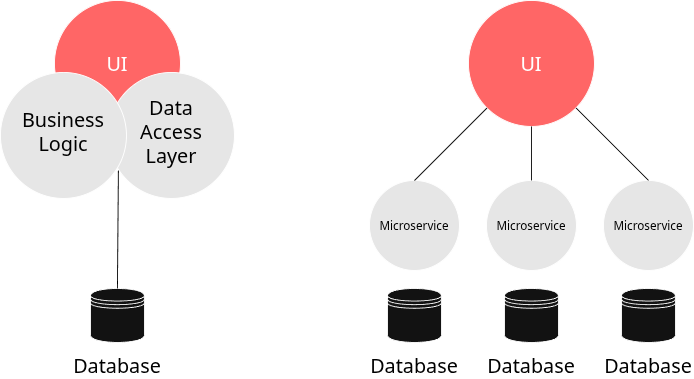
\includegraphics[width=1\textwidth]{images/monolitevsmicro.drawio.png}
    \caption{Confronto strutturale tra architettura Monolitica e a Microservizi [Elaborazione dell'autore]}
    \label{fig:monovsmicro}
\end{figure}

\subsection{Serverless Computing e Function-as-a-Service (FaaS)}
Il Serverless Computing delega al fornitore Cloud la completa gestione dell'allocazione e del provisioning delle risorse computazionali. Come definito da Jonas et al. \cite{BerkeleyServerless}, questo modello combina servizi di backend gestiti con il paradigma Function-as-a-Service (FaaS).
L'operatore fornisce il codice sorgente sotto forma di funzioni, le quali vengono eseguite esclusivamente in reazione a specifici eventi. Questo approccio elimina la manutenzione dei server virtuali e introduce un modello di tariffazione basato sul consumo reale: i costi derivano dal tempo di esecuzione, misurato in millisecondi, e dalla memoria allocata, differenziandosi dai modelli basati sulla disponibilità fissa delle istanze \cite{EC2}.
L'infrastruttura Serverless risulta particolarmente indicata per la gestione di carichi di lavoro discontinui. La presenza di piani tariffari gratuiti per i bassi volumi di traffico consente inoltre di mantenere i costi infrastrutturali prossimi allo zero per gli ambienti di test e per ambienti a basso carico \cite{EivyEconomics}.

\section{Stack Tecnologico per High-Throughput su AWS}
\label{sec:aws_stack}

Amazon Web Services (AWS) eroga una suite di servizi per l'implementazione di architetture Serverless. La selezione di tale fornitore si basa sull'integrazione nativa tra i componenti di calcolo, archiviazione ed elaborazione dati.

\subsection{Compute Layer: AWS Lambda}
AWS Lambda è il servizio di calcolo guidato da eventi che esegue la logica applicativa dell'architettura proposta. Nei sistemi event-driven, il flusso di esecuzione è innescato da variazioni di stato, come il caricamento di un file o la ricezione di una richiesta di rete \cite{EventDrivenArchitecture}.

Le funzioni Lambda sono definite da due proprietà tecniche fondamentali. La prima è l'assenza di stato (stateless): l'ambiente di esecuzione non conserva memoria delle invocazioni precedenti, rendendo necessario l'utilizzo di servizi di storage esterni per la persistenza dei dati.
La seconda proprietà riguarda l'effimerità dell'ambiente di calcolo. Il container che ospita il codice viene istanziato al verificarsi dell'evento e sospeso o terminato al completamento dell'esecuzione. Questa dinamica introduce il fenomeno noto come Cold Start, visibile in Figura \ref{fig:lambda_cold_start}, ovvero una latenza aggiuntiva dovuta al tempo di inizializzazione del runtime durante la prima invocazione, che necessita di specifiche strategie di mitigazione \cite{WangColdStart}.

\begin{figure}[ht!]
    \centering
    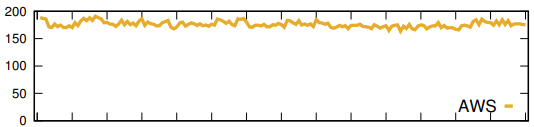
\includegraphics[width=1\textwidth]{images/lambda_cold_start.png}
    \caption{Latenza introdotta dal Cold Start (in ms) nell'arco di 168 ore. La prima invocazione richiede l'inizializzazione del runtime [Fonte: Wang et al., 2018]}
    \label{fig:lambda_cold_start}
\end{figure}

\subsection{Gestione delle API: Amazon API Gateway}
Amazon API Gateway funge da interfaccia per l'esposizione di API su protocollo HTTP/HTTPS, indirizzando le richieste client verso i servizi backend. Le funzionalità principali includono il controllo degli accessi, la limitazione della frequenza delle richieste (throttling) e il monitoraggio del traffico.
L'integrazione tramite Lambda Proxy demanda la formattazione della richiesta e della risposta direttamente alla funzione Lambda associata, semplificando la topologia di instradamento \cite{APIGatewayDoc}.

\subsection{Orchestrazione Eventi e Scheduling: Amazon EventBridge}
L'integrazione tra microservizi asincroni richiede un sistema di messaggistica affidabile. Amazon EventBridge è un bus di eventi che orchestra la comunicazione tra applicazioni e servizi AWS. Esso implementa anche meccanismi di pianificazione, abilitando l'esecuzione di funzioni Lambda a intervalli regolari. Questa caratteristica è essenziale per automatizzare l'avvio di pipeline di estrazione, trasformazione e caricamento (ETL) e processi batch \cite{EventBridgeDoc}.

\begin{figure}[ht!]
    \centering
    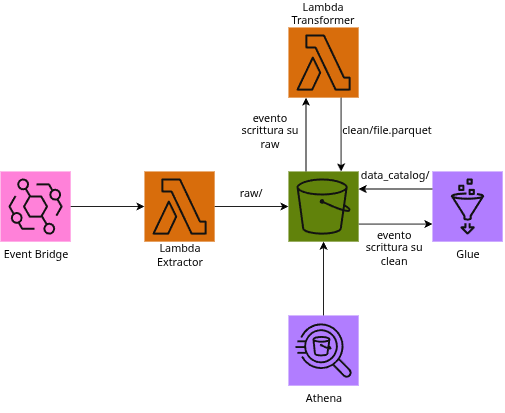
\includegraphics[width=1\textwidth]{images/pipeline-etl.drawio.png}
    \caption{Topologia di una pipeline ETL Serverless. Il flusso evidenzia l'estrazione da S3, la trasformazione via AWS Glue e l'esposizione per l'interrogazione tramite Amazon Athena [Elaborazione dell'autore]}
    \label{fig:pipeline-etl}
\end{figure}

\subsection{Messaggistica Asincrona e Pattern Publish-Subscribe: Amazon SNS}
\label{subsec:sns_dlq}

Nelle architetture a microservizi guidate da eventi, il disaccoppiamento tra i componenti produttori di dati e i componenti consumatori rappresenta un requisito primario per garantire la scalabilità indipendente. Tale disaccoppiamento è tipicamente implementato attraverso il pattern architetturale Publish-Subscribe (Pub/Sub) \cite{PubSubPattern}.

All'interno della piattaforma cloud in esame, questo pattern è concretizzato tramite Amazon Simple Notification Service (SNS). SNS opera come un servizio di messaggistica distribuito che facilita l'invio di messaggi (eventi) da un singolo applicativo (publisher) verso molteplici destinazioni (subscriber) in modalità asincrona. L'entità logica centrale è il \emph{topic}, un canale di comunicazione a cui i publisher inviano i messaggi e a cui i subscriber, come ad esempio funzioni AWS Lambda o endpoint HTTP, si registrano per riceverli \cite{SNS}. Questa configurazione abilita il \emph{fan-out} architetturale: un singolo evento innesca parallelamente molteplici flussi di elaborazione indipendenti, senza che il sistema originario debba gestire la logica di smistamento o conoscere a priori l'identità dei destinatari.

\subsection{Container Registry: Amazon ECR}
Le prassi standard di deployment prevedono l'utilizzo di immagini conformi alle specifiche OCI (Open Container Initiative) per incapsulare il software e le relative dipendenze. Amazon Elastic Container Registry (ECR) ospita le immagini Docker destinate all'esecuzione su AWS Lambda. Questo approccio sfrutta la memorizzazione nella cache dei livelli dell'immagine per ottimizzare i tempi di rilascio e permette l'inclusione di librerie scientifiche complesse, aggirando i limiti dimensionali dei tradizionali pacchetti compressi \cite{ECR}.

\subsection{Gestione della persistenza: Amazon DynamoDB e S3}
La natura stateless delle funzioni Lambda impone l'adozione di sistemi di persistenza in grado di supportare l'elevata concorrenza generata dal livello di calcolo. L'architettura fa affidamento su due soluzioni distinte.
La prima soluzione è Amazon DynamoDB, un database NoSQL di tipo chiave-valore. A differenza dei database relazionali, DynamoDB implementa uno scaling orizzontale, garantendo latenze ridotte anche durante i picchi di traffico. L'utilizzo di questo servizio implica la progettazione di schemi dati specifici, come il Single Table Design, per ottimizzare i percorsi di lettura e scrittura \cite{DynamoDBPaper}.

La seconda soluzione per la persistenza è Amazon S3, un servizio di archiviazione a oggetti. Esso assolve la funzione di repository per i dati non strutturati e agisce come livello di storage persistente per l'implementazione del Data Lake aziendale \cite{S3Doc}.

\subsection{Integrazione Dati: AWS Glue e Amazon Athena}
L'elaborazione dei dati all'interno del sistema richiede l'implementazione di pipeline ETL, il cui scopo è estrarre dati grezzi, trasformarli in formati analitici e caricarli nelle destinazioni finali. A tal fine, vengono impiegati due servizi cooperanti.
Il primo componente è AWS Glue, utilizzato nel sistema principalmente come Data Catalog. In questa architettura, il servizio non viene impiegato per l'esecuzione di cluster Spark \cite{Spark} distribuiti, bensì per il mantenimento di un catalogo di metadati centralizzato che descrive la struttura dei file Parquet \cite{Parquet} depositati nelle zone di archiviazione. L'operatore definisce tramite Glue gli schemi delle tabelle e la gerarchia delle partizioni temporali. Questo meccanismo permette al sistema di mappare i percorsi fisici su S3 verso entità logiche interrogate dai motori di calcolo superiori.
Il secondo componente è Amazon Athena, un motore di query interattivo basato su standard SQL che implementa il paradigma schema-on-read. Il servizio interroga direttamente il Data Catalog di Glue per risolvere la struttura dei dati e i predicati di partizionamento, senza la necessità di caricare preventivamente le informazioni in un database relazionale dedicato. Questa integrazione permette di eseguire analisi complesse sui dataset consolidati nel Data Lake, garantendo prestazioni elevate e una riduzione dei volumi di scansione tramite l'esclusione sistematica delle directory non pertinenti alla finestra temporale analizzata\cite{AWSGlueDoc}.

\subsection{Sicurezza, Identità e Controllo Accessi: IAM e Cognito}
In un'architettura distribuita basata su cloud, la sicurezza e l'isolamento delle risorse richiedono meccanismi di autenticazione e autorizzazione rigorosi, operanti a due livelli distinti: infrastrutturale e applicativo.

Il controllo degli accessi a livello infrastrutturale è governato da AWS Identity and Access Management (IAM). Questo servizio consente di definire in modo granulare quali entità (utenti umani, servizi o risorse di calcolo) dispongano delle autorizzazioni per invocare specifiche API cloud \cite{IAM}. La piattaforma in oggetto applica rigidamente il principio del privilegio minimo (Principle of Least Privilege): ogni microservizio, implementato tramite AWS Lambda, assume un ruolo IAM temporaneo dotato esclusivamente dei permessi strettamente necessari per l'esecuzione del proprio task, riducendo drasticamente la superficie di attacco \cite{LeastPrivilegeCloud}.

A livello applicativo, la gestione delle identità degli utenti finali è demandata ad Amazon Cognito, come illustrato in Figura \ref{fig:cognito-flow}. Cognito agisce come Identity Provider (IdP) e si integra nativamente con API Gateway per validare le richieste in ingresso. Al superamento delle credenziali, il servizio emette token aderenti allo standard JSON Web Token (JWT) \cite{JWT}. API Gateway intercetta questi token, ne verifica crittograficamente la firma e autorizza l'inoltro della richiesta al livello di calcolo sottostante, disaccoppiando così la logica di autenticazione dalla logica di business applicativa \cite{Cognito}.

\begin{figure}[ht!]
    \centering
    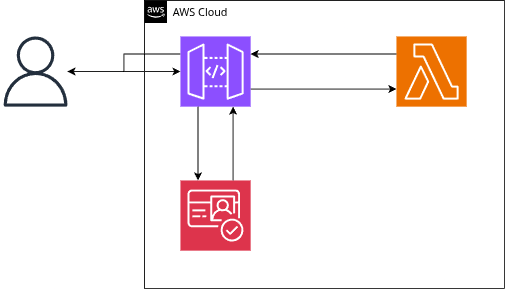
\includegraphics[width=1\textwidth]{images/cognito-api.drawio.png}
    \caption{Schema del flusso di comunicazione tra Api Gateway, Lambda e Cognito [Elaborazione dell'autore]}
    \label{fig:cognito-flow}
\end{figure}

\subsection{Osservabilità e Monitoraggio: Amazon CloudWatch}
La natura effimera e asincrona delle architetture Serverless rende inapplicabili i tradizionali approcci di debugging basati sull'accesso diretto ai server. Di conseguenza, l'osservabilità diviene un requisito architetturale primario per garantire la tracciabilità e la diagnostica del sistema \cite{ServerlessObservability}.

Il servizio Amazon CloudWatch costituisce il fulcro dell'infrastruttura di monitoraggio. Esso espleta tre funzioni essenziali: l'aggregazione centralizzata dei log generati dai container Lambda, la raccolta di metriche prestazionali (quali latenza di esecuzione, tasso di errore e consumo di memoria) e la gestione di allarmi automatizzati \cite{CloudWatch}. L'integrazione di CloudWatch garantisce agli operatori la visibilità sullo stato di salute dell'intero stack applicativo, fornendo i dati necessari per ottimizzare le risorse allocate e risolvere eventuali anomalie operative.

\subsection{Gestione Finanziaria e FinOps: AWS Cost Explorer}

Il paradigma del Cloud Computing trasforma le spese in conto capitale (CapEx) in spese operative (OpEx), introducendo un modello di fatturazione basato sul consumo effettivo (pay-as-you-go). In architetture ad alta densità di eventi, la frammentazione dei componenti serverless rende il monitoraggio finanziario un requisito ingegneristico fondamentale, inquadrato nella disciplina del Cloud Financial Management o FinOps \cite{FinOpsBook}.

L'analisi e l'ottimizzazione della spesa all'interno della piattaforma sono demandate ad AWS Cost Explorer. Questo servizio elabora i dati di telemetria finanziaria fornendo interfacce per la visualizzazione storica, l'identificazione delle anomalie e la previsione dei costi futuri \cite{CostExplorer}.

Un meccanismo essenziale per la ripartizione dei costi in ambienti complessi è costituito dai Cost Allocation Tags. Attraverso l'applicazione di metadati strutturati alle singole risorse infrastrutturali, Cost Explorer aggrega la spesa per dominio logico (ad esempio, per ambiente di rilascio, centro di costo o specifico microservizio). Questa aggregazione abilita il tracciamento granulare del costo per singola transazione e garantisce la tracciabilità economica dell'intero stack applicativo \cite{CostAllocationTags}.

\section{Sviluppo Applicativo: Servizi e Worker}
\label{sec:app_frameworks}

I microservizi sviluppati si dividono in due categorie funzionali: i servizi di backend che espongono API sincrone e i worker asincroni adibiti all'elaborazione dei dati.

\subsection{Sviluppo di Backend API con FastAPI}
La programmazione dei servizi API si avvale di Python, ampiamente adottato per lo sviluppo backend \cite{PythonTrends}, e del framework FastAPI. Oltre al supporto nativo per la concorrenza asincrona, FastAPI utilizza la libreria Pydantic per validare a runtime la struttura dei dati in ingresso e in uscita. Questo meccanismo previene gli errori legati alla tipizzazione e garantisce l'aderenza delle richieste ai formati attesi \cite{FastAPIDoc}. Il framework genera inoltre autonomamente la specifica OpenAPI, facilitando la documentazione delle interfacce.

\subsection{Elaborazione Asincrona: Event-Driven Workers}
A differenza dei servizi API, che seguono un paradigma richiesta-risposta sincrono, i worker operano in modalità totalmente asincrona e disaccoppiata, come illustrato nello schema in Figura \ref{fig:pipeline-etl}. In un'architettura guidata da eventi, un worker è un componente software incaricato di eseguire operazioni ad alta intensità computazionale o processi di background, quali le trasformazioni ETL (Extract, Transform, Load), la pulizia dei dati o la sincronizzazione con sistemi di terze parti.

L'esecuzione di un worker non è innescata da una chiamata HTTP diretta, bensì da eventi di sistema emessi dall'infrastruttura cloud. Tali eventi includono il caricamento di un oggetto in un bucket Amazon S3, la pubblicazione di un messaggio su un topic SNS, o lo scoccare di una regola cronologica definita in Amazon EventBridge. Questo radicale disaccoppiamento garantisce la scalabilità indipendente dei processi di elaborazione dati, impedendo che i carichi di lavoro intensivi saturino le risorse o aumentino la latenza delle interfacce esposte agli utenti \cite{EventDrivenArchitecture}.

\subsection{Adattamento al runtime Lambda: Mangum e Lambda RIC}
L'esecuzione del codice all'interno dell'ambiente AWS Lambda necessita di moduli di interfaccia specifici per colmare la differenza tra i protocolli standard e gli eventi proprietari del cloud provider.
Per i servizi API, viene utilizzato Mangum, come illustrato in Figura \ref{fig:mangum}. Questo adattatore converte i payload JSON forniti da API Gateway in richieste HTTP standardizzate, permettendo l'esecuzione di applicazioni conformi allo standard ASGI (come FastAPI) all'interno di Lambda \cite{MangumDoc}.
Per i worker asincroni, si impiega l'AWS Lambda Runtime Interface Client (RIC). Tale libreria espone l'API del runtime Lambda ai container Docker personalizzati, consentendo l'esecuzione di script Python generici in risposta a eventi non HTTP.

\begin{figure}[ht!]
    \centering
    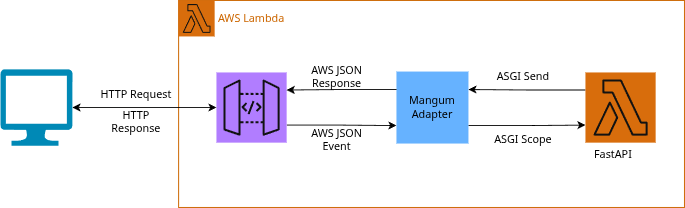
\includegraphics[width=1\textwidth]{images/mangum.drawio.png}
    \caption{Schema del flusso di adattamento tramite Mangum. L'evento AWS viene tradotto in una richiesta compatibile con l'interfaccia ASGI [Elaborazione dell'autore]}
    \label{fig:mangum}
\end{figure}

\section{Infrastructure as Code con Terraform}
\label{sec:terraform_iac}

La configurazione manuale tramite interfaccia grafica di infrastrutture complesse risulta soggetta a errori e non replicabile. L'approccio Infrastructure as Code (IaC) mitiga queste problematiche definendo l'infrastruttura tramite file di testo strutturati.

\subsection{Il paradigma dell'Infrastruttura Immutabile}
L'IaC abilita il controllo di versione per l'infrastruttura tramite Git \cite{Git}, assoggettandola ai medesimi processi di revisione del codice software. Strumenti come Terraform utilizzano un approccio dichiarativo: l'ingegnere specifica lo stato finale atteso per le risorse cloud, ed è responsabilità del software calcolare il piano di esecuzione e applicare le mutazioni necessarie per allineare l'ambiente reale alla configurazione definita \cite{IaCGuerriero}.

\subsection{Modularità e Gestione dello Stato}
Terraform mappa la configurazione dichiarata con le risorse allocate sul cloud attraverso un file di stato remoto. Al fine di standardizzare la creazione delle risorse ed evitare la duplicazione del codice, l'architettura fa ampio uso dei moduli Terraform. L'incapsulamento delle definizioni infrastrutturali all'interno di moduli riutilizzabili assicura che ogni nuovo servizio ereditato rispetti intrinsecamente i parametri di sicurezza e di tracciamento aziendali \cite{TerraformUpAndRunning}.

\subsection{Orchestrazione dell'Infrastruttura e principio DRY: Terragrunt}

La gestione di architetture multi-ambiente tramite il solo framework Terraform impone la replicazione del codice dichiarativo per ogni contesto di esecuzione, incrementando il debito tecnico. Per risolvere questa limitazione strutturale, l'architettura si avvale di Terragrunt. Terragrunt è un orchestratore open-source che agisce come livello di astrazione (wrapper) superiore rispetto all'eseguibile nativo di Terraform. Il software intercetta i comandi operativi impartiti dall'utente e inietta dinamicamente i parametri di configurazione prima di delegarne l'esecuzione al motore di provisioning sottostante.

L'adozione di questo orchestratore abilita l'applicazione rigorosa del principio ingegneristico Don't Repeat Yourself. L'ingegnere definisce la logica di creazione delle risorse una singola volta all'interno di moduli Terraform generici e isolati. Successivamente, tramite i file di configurazione proprietari di Terragrunt, il sistema instaura delle gerarchie di ereditarietà. Le directory che mappano gli ambienti fisici (come lo sviluppo o la produzione) si limitano a ereditare la logica del modulo base, sovrascrivendo unicamente le variabili specifiche del contesto, quali il dimensionamento computazionale o i puntamenti di rete.

Oltre alla deduplicazione del codice, l'orchestratore automatizza la gestione dello stato remoto (remote state). Terragrunt genera e configura dinamicamente i backend di archiviazione per ogni singolo ambiente, prevenendo errori di configurazione manuale che causerebbero la corruzione dello stato infrastrutturale. Questa standardizzazione assicura che i file di stato rimangano rigorosamente segregati per ciascun account cloud aziendale.

Infine, il framework introduce costrutti dichiarativi espliciti per la risoluzione delle dipendenze inter-modulo. Terraform nativamente non permette di orchestrare moduli situati in directory distinte; Terragrunt supera questo ostacolo calcolando il grafo topologico dell'intera infrastruttura. Questa funzionalità permette al sistema di passare le variabili di output di un modulo (come l'identificativo di una rete appena creata) come parametri di input per un modulo dipendente (come un cluster di calcolo), garantendo il rispetto della corretta sequenza logica durante le operazioni di rilascio. \cite{Terragrunt}

\section{Automazione del Ciclo di Vita del Software (SDLC)}
\label{sec:sdlc}

L'automazione del ciclo di sviluppo (SDLC) si prefigge di ottimizzare l'iterazione tra la stesura del codice, la sua validazione e la successiva messa in produzione.

\subsection{Containerizzazione e parità degli ambienti}
La distribuzione del codice tramite archivi compressi comporta limitazioni operative, quali la difficoltà di includere librerie pre-compilate e l'impossibilità di garantire l'identità tra l'ambiente di sviluppo e quello di esecuzione. L'adozione dello standard Docker permette di incapsulare l'applicativo, le librerie e il sistema operativo di base all'interno di un'immagine immutabile. Questo garantisce la parità degli ambienti, assicurando che il comportamento del software validato localmente dallo sviluppatore rimanga coerente una volta rilasciato nell'infrastruttura di produzione \cite{DockerDoc}.

\subsection{Emulazione Cloud per lo sviluppo locale: LocalStack}
Un ostacolo intrinseco allo sviluppo di applicazioni Cloud-Native è la latenza introdotta dalla necessità di distribuire ogni singola modifica sull'infrastruttura remota per poterne verificare il funzionamento. Questa dipendenza dilata i tempi del ciclo di iterazione locale, definito come la sequenza di scrittura, compilazione e test del codice \cite{RedHatInnerLoop}.
Per ripristinare un ciclo di sviluppo rapido, viene impiegato LocalStack, un emulatore che espone API compatibili con i principali servizi AWS. L'esecuzione di LocalStack tramite container permette di simulare l'interazione tra componenti come Lambda, DynamoDB e S3 direttamente sulla postazione di lavoro, abilitando il collaudo del software in assenza di connettività verso il cloud e abbattendo i tempi di attesa \cite{LocalStackPaper}.

\subsection{Continuous Integration e Delivery (CI/CD)}
Le pratiche di Continuous Integration e Continuous Delivery automatizzano le fasi di test e rilascio. Tramite piattaforme come GitHub Actions, il caricamento di nuovo codice sorgente innesca l'esecuzione sequenziale di test unitari, la compilazione delle immagini Docker e il caricamento sul registro ECR. Questo flusso di lavoro automatizzato esclude le operazioni manuali dai processi di deployment, garantendo la riproducibilità tecnica dei rilasci \cite{AccelerateBook}.

\section{Evoluzione dell'Automazione: LLM e Model Context Protocol}
\label{sec:mcp_background}

La recente diffusione dei Large Language Models (LLM) ha introdotto nuovi paradigmi nell'ambito dell'ingegneria del software, estendendo le capacità di automazione oltre la generazione statica di codice \cite{LLMSoftwareEngineering}. Tuttavia, l'efficacia di tali modelli in contesti aziendali è storicamente limitata dal loro isolamento rispetto agli ambienti di esecuzione locali e alle infrastrutture proprietarie.

Per superare tale limitazione, la letteratura tecnica ha formalizzato il concetto di \textit{Tool Use} (o \textit{Function Calling}), ovvero la capacità di un modello di delegare l'esecuzione di calcoli deterministici o l'interazione con sistemi esterni a script predefiniti \cite{LLMTool}.
In questo contesto si inserisce il Model Context Protocol (MCP), uno standard aperto introdotto per uniformare la comunicazione tra le applicazioni di intelligenza artificiale (Client) e le sorgenti di dati o gli strumenti operativi (Server) \cite{MCP}.

Il protocollo MCP adotta un'architettura client-server standardizzata, definendo un insieme rigoroso di primitive per l'esposizione di risorse, prompt e strumenti (Tools). Tale astrazione permette agli ambienti di sviluppo integrati (IDE) dotati di agenti conversazionali di interrogare un server MCP locale o remoto per scoprire quali operazioni infrastrutturali siano disponibili, ottenendo in risposta il relativo schema JSON dei parametri richiesti.
Al fine di accelerare lo sviluppo di server compatibili con tale standard, l'ecosistema Python mette a disposizione librerie come FastMCP \cite{FastMCP}. Questi framework astraggono la complessità del trasporto a basso livello (gestito tipicamente tramite stdio o Server-Sent Events), consentendo all'ingegnere di mappare le funzioni Python direttamente sulle interfacce del protocollo tramite l'impiego di decoratori sintattici, garantendo la validazione automatica dei tipi in ingresso e in uscita.

\begin{figure}[ht!]
    \centering
    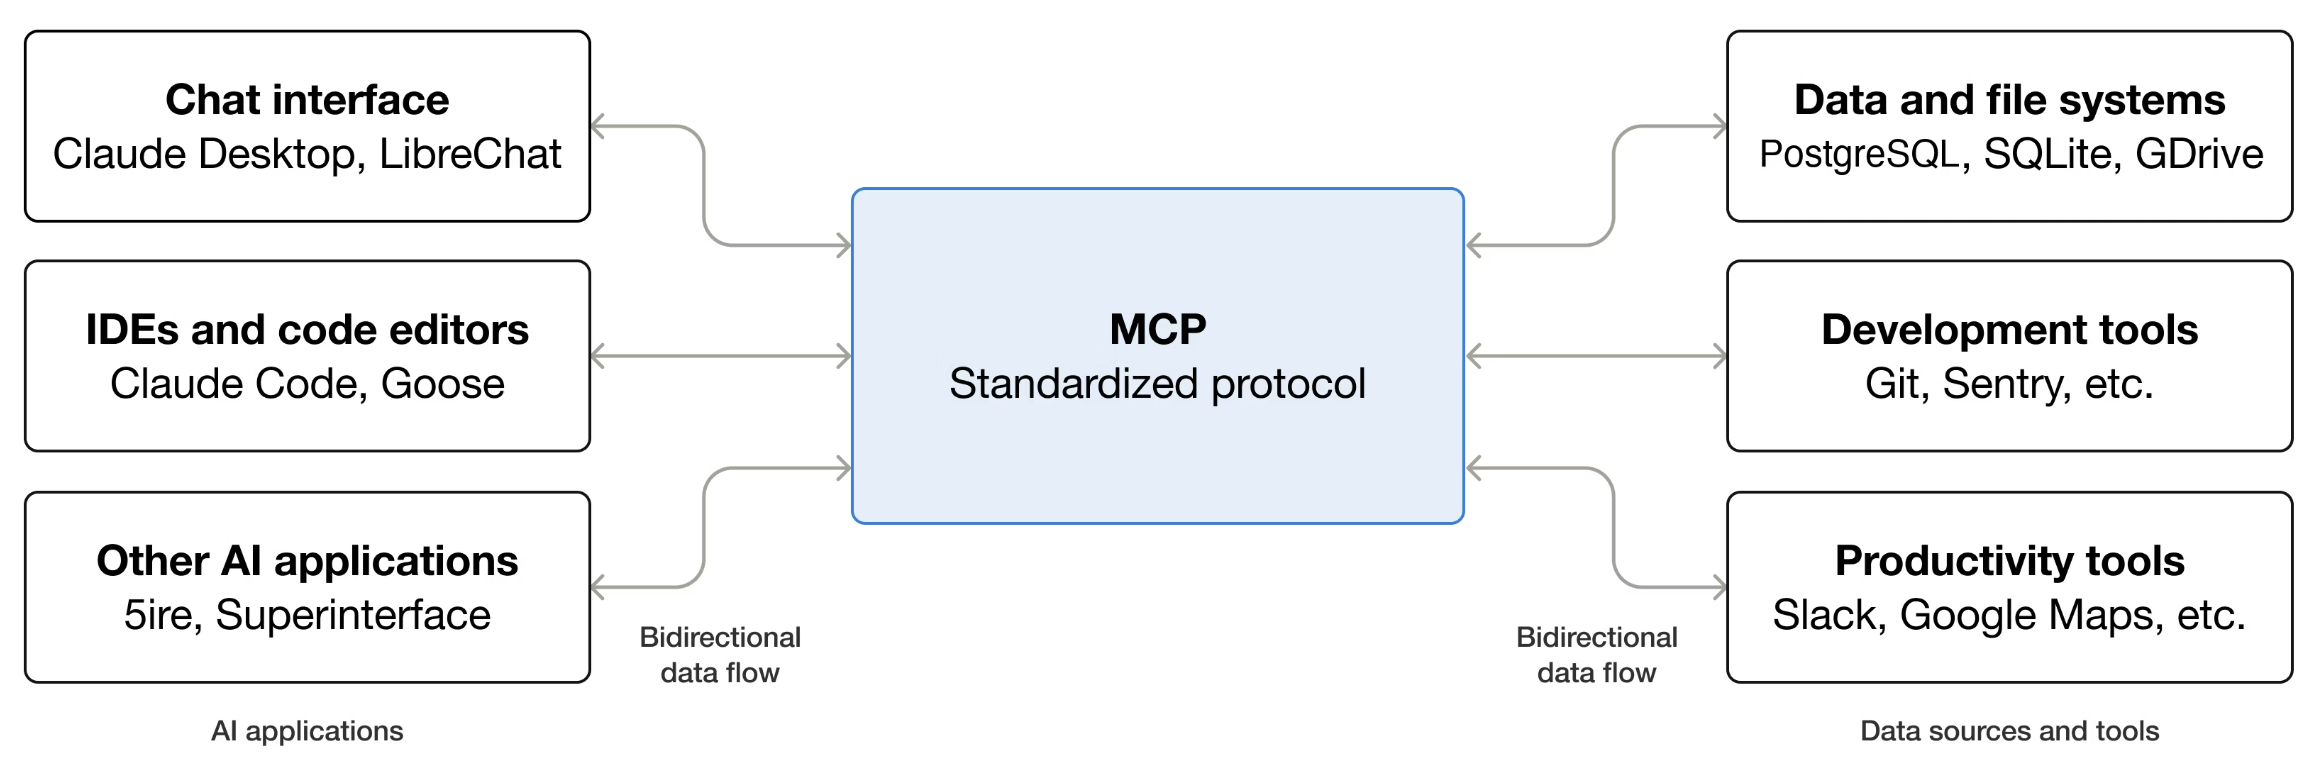
\includegraphics[width=1\textwidth]{images/mcp.png}
    \caption{MCP come protocollo di comunicazione standard tra LLM e tools [Fonte: modelcontextprotocol.io \cite{MCP}]}
    \label{fig:mcp}
\end{figure}

\chapter{Analisi e Design}
\label{chap:analisi}

Il presente capitolo illustra l'analisi dei requisiti e la progettazione architetturale del sistema. La struttura del capitolo segue un approccio incrementale: si definiscono i requisiti operativi, si progetta l'infrastruttura Cloud di base (strategia Multi-Account e Serverless), si modella il livello di persistenza e i flussi dati (Event-Driven, S3, DynamoDB) e si definisce l'architettura interna del software applicativo. Infine, vengono delineati i processi di automazione e le pratiche di Infrastructure as Code necessari a governare il ciclo di vita del software. L'obiettivo è fornire una giustificazione formale e ingegneristica per ogni scelta tecnologica, ponendo le basi per l'implementazione descritta nel capitolo successivo.

\section{Analisi del Contesto Operativo e Definizione dei Requisiti}
\label{sec:analisi_contesto}

L'analisi del contesto operativo esamina le criticità intrinseche alle infrastrutture tradizionali impiegate nel settore dell'advertising digitale. Questo dominio applicativo impone l'elaborazione di elevati volumi di dati in tempo reale e richiede la gestione di carichi di rete altamente variabili. L'ispezione delle architetture legacy evidenzia limitazioni strutturali derivanti dall'eterogeneità dei servizi e dall'esecuzione parzialmente manuale delle procedure di rilascio. L'assenza di un sistema di versionamento dichiarativo impedisce la tracciabilità delle modifiche infrastrutturali e compromette la riproducibilità degli ambienti operativi. Tale debito tecnico costringe i sistemi a un'allocazione statica delle risorse computazionali, la quale risulta indipendente dal carico effettivo e incapace di adattarsi dinamicamente alle fluttuazioni del traffico.

L'identificazione di questi colli di bottiglia operativi determina la formulazione di tre requisiti architetturali primari per la progettazione del nuovo sistema Cloud-Native.

Il primo requisito definisce la necessità di una scalabilità elastica. L'architettura deve allocare e deallocare dinamicamente le risorse computazionali per assorbire i picchi di traffico imprevisti. Questa elasticità deve garantire latenze di elaborazione minime senza richiedere alcun intervento di ridimensionamento manuale da parte di un operatore.

Il secondo vincolo architetturale impone l'isolamento degli ambienti operativi. Il sistema deve garantire una separazione logica e fisica rigorosa tra le risorse destinate alla programmazione, alle fasi di collaudo e all'ambiente di produzione. Tale segregazione previene interferenze tra i carichi di lavoro e assicura che i test non impattino le prestazioni dei servizi esposti agli utenti finali.

Infine, il terzo requisito prescrive la tracciabilità e l'automazione integrale dei flussi operativi. La progettazione deve vincolare la gestione dei componenti cloud all'utilizzo di codice dichiarativo, trattando l'infrastruttura alla stregua del software applicativo. Parallelamente, il sistema deve implementare pipeline automatizzate per disciplinare i processi di integrazione e di rilascio continuo (CI/CD), eliminando le operazioni manuali.

\section{Progettazione dell'Infrastruttura Cloud}
\label{sec:design_infrastruttura}

Per soddisfare i requisiti prestazionali, l'architettura si basa sul paradigma Serverless \cite{BerkeleyServerless}, implementato tramite Amazon Web Services (AWS). Questa scelta rimuove l'onere della gestione di macchine virtuali e introduce un modello di costo calcolato sui tempi di esecuzione effettivi.

Come illustrato nello schema logico in Figura \ref{fig:architettura_serverless_overview}, per garantire la modularità l'architettura è stata concettualmente divisa in due categorie funzionali: i servizi di backend (Services), deputati all'esposizione di interfacce di programmazione sincrone, e i componenti asincroni (Workers), dedicati all'elaborazione in background dei dati.

\begin{figure}[htbp]
    \centering
    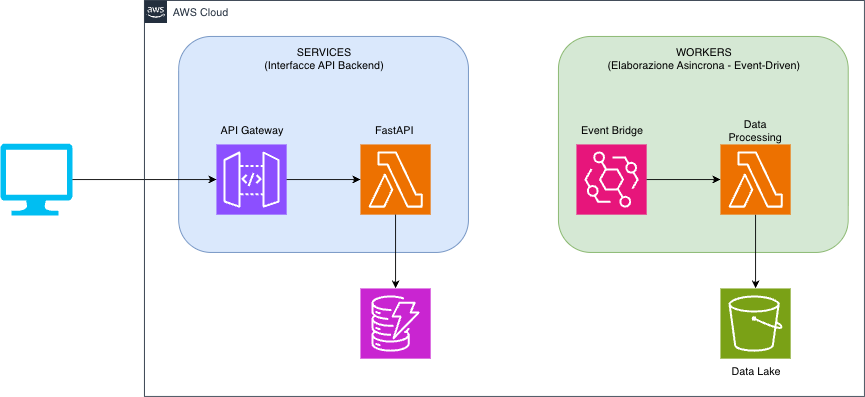
\includegraphics[width=1\textwidth]{images/services_workers.drawio.png}
    \caption{Schema concettuale dell'architettura Serverless su AWS, illustrante la separazione tra Services (interfacce sincrone) e Workers (elaborazione asincrona) [Elaborazione dell'autore].}
    \label{fig:architettura_serverless_overview}
\end{figure}

\subsection{Strategia Multi-Account e Segregazione delle Risorse}

L'impiego di un singolo account AWS per l'intero ciclo di vita del software estende pericolosamente il dominio di faglia in caso di incidenti e complica il controllo degli accessi. La progettazione ha quindi previsto una strategia Multi-Account, la cui topologia è rappresentata in Figura \ref{fig:aws_multi_account_topology}, strutturata su tre ambienti isolati: Sviluppo (Dev), Produzione (Prod) e Condiviso (Shared).

Gli account Dev e Prod sono copie speculari, garantendo che le configurazioni validate in sviluppo si comportino in modo deterministico in produzione. L'account Shared agisce come nodo centralizzato, ospitando le risorse accessibili trasversalmente: i registri Amazon ECR \cite{ECR} per le immagini Docker e i bucket S3 per gli artefatti statici. Questa topologia centralizzata previene la duplicazione dei pacchetti e permette ai flussi di deployment di prelevare gli artefatti da un'unica sorgente sicura.

\begin{figure}[htbp]
    \centering
    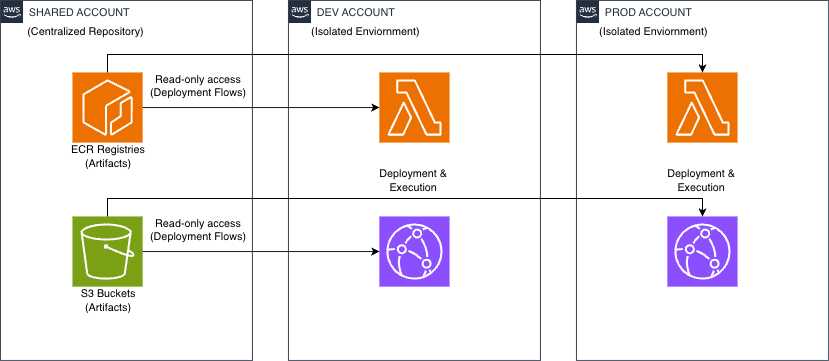
\includegraphics[width=0.95\textwidth]{images/aws-multi-account.drawio.png}
    \caption{Topologia della strategia Multi-Account su AWS. L'account Shared centralizza gli artefatti, referenziati in sola lettura per il deployment negli ambienti isolati [Elaborazione dell'autore].}
    \label{fig:aws_multi_account_topology}
\end{figure}

\section{Progettazione del Livello Dati e Flussi Asincroni}
\label{sec:design_dati}

L'architettura separa le responsabilità tra l'archiviazione di volumi massivi per l'analisi e la memorizzazione transazionale a bassa latenza, introducendo un netto disaccoppiamento tra produttori e consumatori di dati.

\subsection{Decomposizione Event-Driven ed ETL Serverless}

I processi di elaborazione dati sono stati re-ingegnerizzati applicando il pattern Event-Driven \cite{EventDrivenArchitecture}. I flussi di estrazione e trasformazione (ETL) sono composti da microservizi specializzati asincroni.
Come delineato in Figura \ref{fig:pipeline-etl}, i servizi di estrazione depositano i dati grezzi in un Data Lake su Amazon S3 \cite{S3Doc}. L'inserimento di un file innesca automaticamente l'esecuzione di funzioni AWS Lambda \cite{AWSLambdaDoc} o processi AWS Glue \cite{AWSGlueDoc}. Questi componenti applicano le regole di pulizia e salvano i dati nel formato colonnare Parquet.

\begin{figure}[ht!]
    \centering
    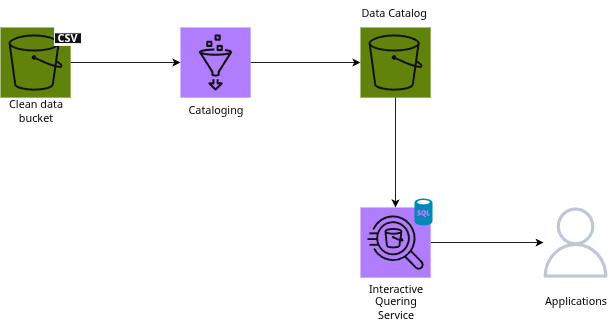
\includegraphics[width=1\textwidth]{images/elaborazione-serverless.drawio.png}
    \caption{Pipeline di elaborazione dati Serverless. AWS Glue trasforma i dati grezzi su S3 rendendoli interrogabili tramite Athena [Elaborazione dell'autore].}
    \label{fig:pipeline-etl}
\end{figure}

\subsection{Partizionamento Hive-Style del Data Lake}

Per ottimizzare le prestazioni e mitigare i costi operativi, il Data Lake è diviso in due zone logiche distinte: Raw (per i dati estratti nel formato originale) e Clean (per i dati trasformati e standardizzati). I dati immagazzinati nella zona Clean sono archiviati applicando rigorosamente un partizionamento Hive-style \cite{HiveStyle}. Questo paradigma organizza i file in percorsi gerarchici auto-descrittivi basati su coordinate temporali, ad esempio, \texttt{anno=2024/mese=10/giorno=25/}, come visualizzato nella gerarchia di Figura \ref{fig:s3_hive_partitioning}.

\begin{figure}[htbp]
    \centering
    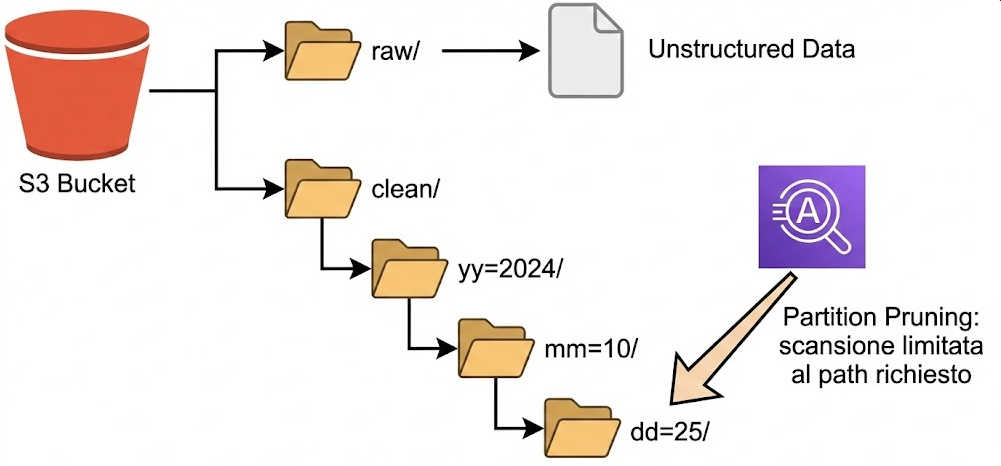
\includegraphics[width=1\textwidth]{images/partition-pruning.png}
    \caption{Struttura gerarchica del Data Lake su Amazon S3 basata su partizionamento Hive-style. L'organizzazione abilita il partition pruning da parte di Amazon Athena [Elaborazione dell'autore].}
    \label{fig:s3_hive_partitioning}
\end{figure}

Questo design logico permette ad Amazon Athena \cite{Athena} di eseguire l'operazione di partition pruning, ignorando sistematicamente le directory non pertinenti alla query SQL in esecuzione. Per quantificare l'impatto architetturale di tale scelta, si consideri l'esecuzione di un'interrogazione analitica tipica per l'estrazione delle metriche giornaliere relative a una specifica campagna pubblicitaria:

\begin{lstlisting}[language=SQL]
SELECT campaign_id, SUM(impressions) AS total_impressions
FROM impressions_table
WHERE campaign_id = 'ABC-123' 
  AND year = '2024' AND month = '10' AND day = '25';
\end{lstlisting}

In un Data Lake privo di partizionamento logico, il motore di query distribuito è costretto a leggere sequenzialmente l'intero volume di dati archiviato nel bucket Amazon S3 per individuare i record. Assumendo un volume di 1 Terabyte (TB) di dati storici, l'operazione comporta la scansione dell'intero Terabyte, incorrendo nel costo fisso per TB associato ad Athena.

Sfruttando il partizionamento, il motore interroga preventivamente il catalogo dati per risolvere i predicati della clausola WHERE associati alle chiavi di partizione. Questa operazione permette ad Athena di accedere esclusivamente al prefisso S3 isolato. Se il volume di dati generato nella singola giornata ammonta a 10 Gigabyte (GB), il sistema scansiona esclusivamente tale frazione, traducendosi in una riduzione del 99\% dei dati elaborati, con un conseguente abbattimento dei costi e della latenza.

\subsection{Modellazione NoSQL: Single Table Design}

La persistenza dello stato transazionale dei microservizi è demandata ad Amazon DynamoDB \cite{DynamoDBPaper}. La progettazione adotta massicciamente il Single Table Design \cite{SingleTableDesign}, memorizzando entità eterogenee all'interno di un'unica tabella, come esemplificato in Figura \ref{fig:single-table-design}. Sfruttando chiavi primarie composite (Partition Key e Sort Key) progettate ad hoc, il sistema recupera relazioni complesse con una singola operazione di lettura, minimizzando il consumo di Read Capacity Units (RCU).

\begin{figure}[ht!]
    \centering
    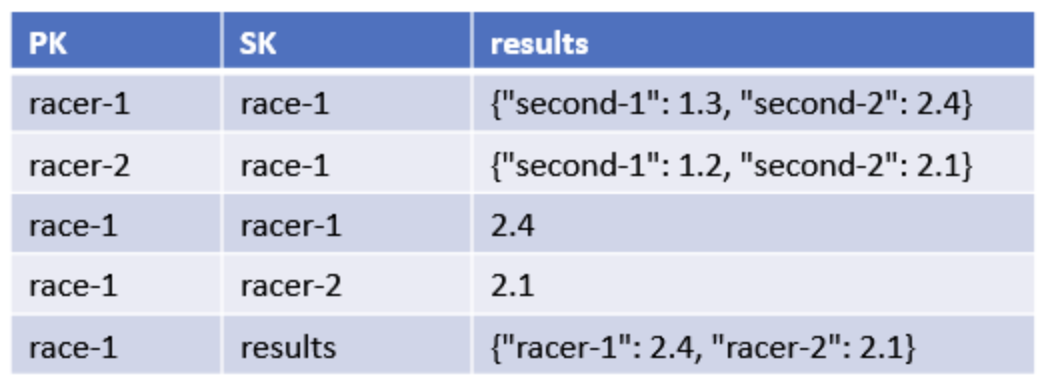
\includegraphics[width=1\textwidth]{images/single-table-design.png}
    \caption{Esempio di Single Table Design per la memorizzazione di entità eterogenee in una singola tabella \cite{SingleTableDesign}.}
    \label{fig:single-table-design}
\end{figure}

\section{Progettazione dei Servizi Applicativi}
\label{sec:design_backend}

I microservizi che espongono API sincrone richiedono un rigore strutturale per garantire la manutenibilità del codice e la stabilità delle interfacce pubbliche.

\subsection{Framework API e Validazione dei Dati}
\label{subsec:framework_fastapi}

Per lo sviluppo dei microservizi è stato selezionato il framework Python FastAPI \cite{FastAPIDoc}. In questo contesto, la libreria Pydantic assume un ruolo centrale per l'ispezione statica dei tipi e la validazione a runtime. Ogni payload JSON deve superare una convalida formale contro schemi predefiniti.

L'implementazione di questo meccanismo si fonda sulla definizione di Data Transfer Object (DTO). Di seguito è illustrato un modello rappresentativo per l'accettazione di un payload relativo a una campagna pubblicitaria:

\begin{lstlisting}[language=python]
from pydantic import BaseModel, Field, HttpUrl
from datetime import date

class CampaignCreateDTO(BaseModel):
    campaign_name: str = Field(..., min_length=3, max_length=100)
    budget: float = Field(..., gt=0)
    target_url: HttpUrl
    start_date: date
\end{lstlisting}

Quando il microservizio riceve una richiesta HTTP POST, il framework esegue la conversione automatica dei tipi e la validazione dei vincoli dichiarativi. Qualora il payload non rispetti i vincoli, ad esempio un budget negativo, l'istanza dell'oggetto non viene creata e la logica di business non viene invocata. Il framework genera in automatico una risposta HTTP 422, fornendo un corpo JSON che localizza l'errore:

\begin{lstlisting}
{
  "detail": [
    {
      "loc": ["body", "budget"],
      "msg": "Input should be greater than 0",
      "type": "greater_than",
      "ctx": {"gt": 0}
    }
  ]
}
\end{lstlisting}

Questa tipologia di validazione minimizza la necessità di scrivere codice procedurale per la gestione delle eccezioni.

\subsection{Architettura Interna: Clean Architecture e Dependency Injection}

Per prevenire un elevato accoppiamento strutturale, la base di codice aderisce ai principi della Clean Architecture \cite{CleanArchitecture}. Come mostrato in Figura \ref{fig:clean_architecture_fastapi}, il software è stratificato in tre livelli funzionali.

\begin{figure}[htbp]
    \centering
    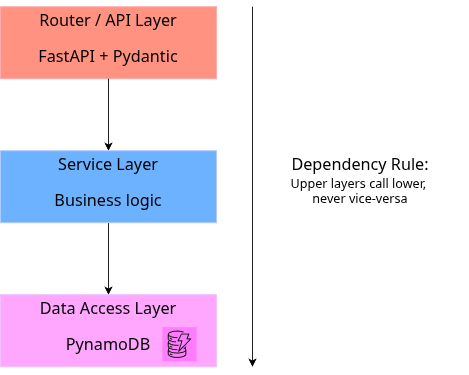
\includegraphics[width=1\textwidth]{images/clean-architecture.drawio.png}
    \caption{Stratificazione interna dei microservizi secondo i principi della Clean Architecture. Il flusso di controllo è unidirezionale dal livello di presentazione verso il livello di accesso ai dati [Elaborazione dell'autore].}
    \label{fig:clean_architecture_fastapi}
\end{figure}

Il primo strato è il Router Layer, che gestisce esclusivamente il routing HTTP. Il secondo è il Service Layer, contenente la logica di business agnostica rispetto a database e framework web. Il terzo è il Repository Layer, che incapsula le interazioni con S3 e DynamoDB.
Il passaggio di informazioni e dipendenze tra i livelli sfrutta il pattern Dependency Injection. Oltre all'iniezione delle dipendenze strutturali, il meccanismo è impiegato per le validazioni di dominio preliminari, permettendo ai controller di rimanere snelli.

\section{Osservabilità e Gestione delle Anomalie}
\label{sec:design_observability}

In ambienti Serverless distribuiti, l'assenza di server fisici impone l'adozione di meccanismi di tracciamento centralizzati e proattivi. Tutti i microservizi implementano un logger egualmente configurato che produce output in formato JSON strutturato, incanalato in Amazon CloudWatch. 

Per la gestione degli errori nei flussi asincroni, il design prevede l'utilizzo di Dead Letter Queue (DLQ), come illustrato in Figura \ref{fig:observability_dlq_flow}. I messaggi non elaborabili, dopo aver esaurito la politica di retry, vengono isolati in questa coda. L'evento di inserimento innesca notifiche tramite EventBridge \cite{EventBridgeDoc} verso i canali operativi aziendali, minimizzando i tempi di rilevamento.

\begin{figure}[htbp]
    \centering
    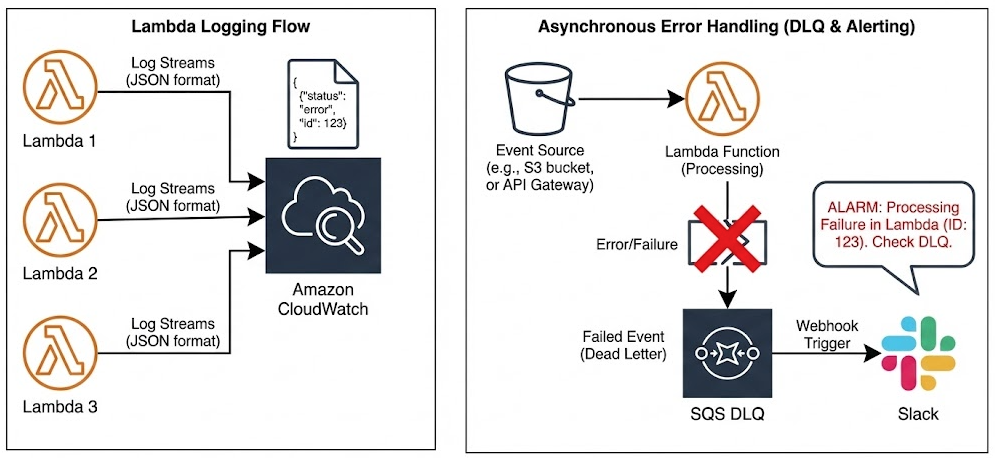
\includegraphics[width=1\textwidth]{images/dlq-logging.png}
    \caption{Flusso architetturale della telemetria. I log strutturati confluiscono in Amazon CloudWatch; i messaggi non processabili vengono isolati in una Dead Letter Queue (DLQ) innescando sistemi di notifica [Elaborazione dell'autore].}
    \label{fig:observability_dlq_flow}
\end{figure}

\section{Automazione e Infrastructure as Code (IaC)}
\label{sec:design_automazione}

La garanzia di riproducibilità è assicurata dalla traduzione dell'intera infrastruttura in codice dichiarativo e dall'automazione delle pipeline di rilascio.

\subsection{Topologia Architetturale del Codice IaC}

Le risorse cloud sono modellate tramite Terraform \cite{IaCGuerriero, TerraformUpAndRunning}. Per agevolare la governance, la progettazione adotta un singolo repository infrastrutturale centralizzato. Tuttavia, la gestione di un'infrastruttura di livello enterprise tramite un singolo file di stato (state file) monolitico costituisce un anti-pattern ingegneristico. Un file di stato di grandi dimensioni dilata i tempi di calcolo del grafo delle dipendenze e amplifica il raggio di impatto (blast radius) in caso di corruzione accidentale dello stesso.

Per mitigare tali criticità, la topologia del repository implementa un'architettura a strati, come schematizzato nella Figura \ref{fig:iac_terraform_workflow}. Il design impone una netta segregazione logica tra la definizione astratta delle risorse e la loro effettiva istanziazione negli ambienti cloud di destinazione.

\begin{figure}[htbp]
\centering
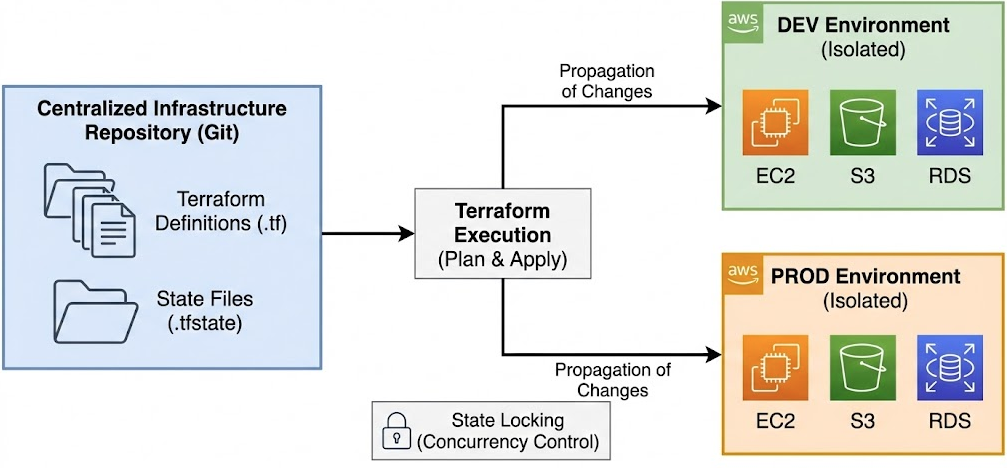
\includegraphics[width=1\textwidth]{images/flusso_iac.png}
\caption{Flusso di lavoro Infrastructure as Code: versionamento dello stato dichiarativo e propagazione delle modifiche tramite Terraform [Elaborazione dell'autore].}
\label{fig:iac_terraform_workflow}
\end{figure}

Il primo livello di questa astrazione è costituito dai moduli riutilizzabili. Ogni modulo incapsula i dettagli implementativi di un dominio architetturale specifico, come il provisioning di un cluster containerizzato o la configurazione di un database, ed espone esclusivamente un'interfaccia controllata di variabili in ingresso. Questo approccio garantisce che la logica di creazione delle risorse venga scritta e sottoposta a revisione una singola volta.

Per governare la topologia a strati e garantire il rispetto del principio DRY (\textit{Don't Repeat Yourself}), la progettazione architetturale prescrive l'adozione dell'orchestratore Terragrunt. Il livello di istanziazione (definito \textit{Live Environment}) delega a questo strumento la mappatura della topologia degli account AWS isolati (\texttt{dev}, \texttt{prod} e \texttt{shared}). Al fine di prevenire derive di configurazione (\textit{configuration drift}) tra i diversi ambienti, il design centralizza le definizioni, evitando la duplicazione manuale del codice dichiarativo.

Il sistema adotta un modello a ereditarietà basato sui file di configurazione dell'orchestratore. Un livello base comune definisce la struttura logica dell'intera infrastruttura, suddivisa in moduli dipendenti e sequenziali: le fondamenta di rete, i sistemi di messaggistica, lo strato di persistenza e il livello applicativo. Le directory relative ai singoli ambienti ereditano questo template tramite specifiche direttive di inclusione, sovrascrivendo unicamente i parametri operativi di competenza, quali il dimensionamento delle istanze computazionali, i limiti di auto-scaling o i riferimenti ai certificati crittografici.

Infine, la scomposizione dello stato infrastrutturale in strati funzionali indipendenti assicura che l'aggiornamento di un componente isolato, ad esempio, un singolo microservizio, non inneschi la lettura o la validazione dello stato dell'infrastruttura di rete o dei database sottostanti. Questa granularità ottimizza le prestazioni delle pipeline di integrazione continua, abilitando aggiornamenti paralleli e riducendo il raggio d'impatto in caso di anomalie durante le procedure di rilascio.

\subsection{Containerizzazione e Pipeline GitOps}

L'incapsulamento del software avviene tramite immagini Docker \cite{DockerDoc}, garantendo parità crittografica tra gli artefatti testati in sviluppo e quelli rilasciati in produzione. 

Il flusso di rilascio, descritto nella Figura \ref{fig:trunk_based_cicd}, implementa il Trunk-Based Development \cite{AccelerateBook}, in cui lo sviluppo converge rapidamente verso un singolo ramo \texttt{main}. Le pipeline CI/CD, basate sul paradigma GitOps \cite{GitOps}, sono innescate dal versionamento semantico definito dai Conventional Commits \cite{ConventionalCommits}. L'artefatto compilato è univoco e viene promosso progressivamente dagli ambienti di test alla produzione senza necessitare di successive ricompilazioni.

\begin{figure}[htbp]
    \centering
    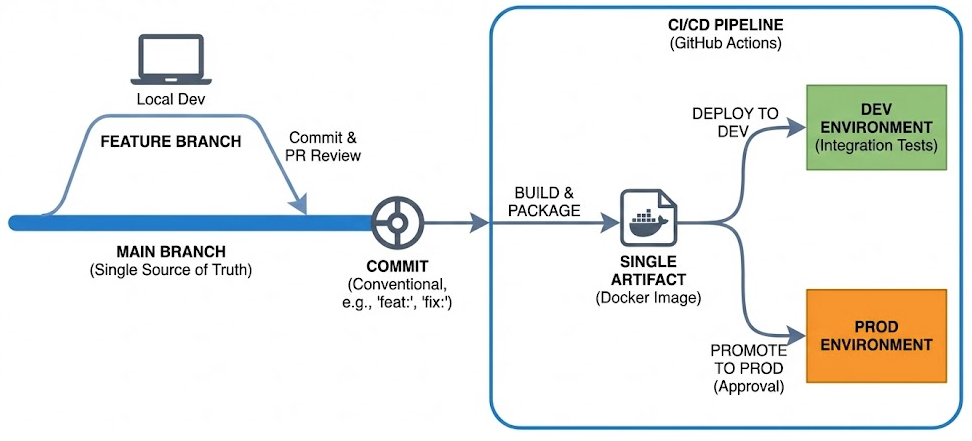
\includegraphics[width=1\textwidth]{images/flusso-commit.png}
    \caption{Flusso architetturale della pipeline CI/CD basata sul Trunk-Based Development. L'unione sul branch principale innesca la generazione dell'artefatto promosso nei vari ambienti [Elaborazione dell'autore].}
    \label{fig:trunk_based_cicd}
\end{figure}

\subsection{Design dell'Interfaccia MCP per l'Automazione Infrastrutturale}

L'adozione rigorosa dell'Infrastructure as Code (IaC) e dei flussi CI/CD basati su GitOps assicura la stabilità e la sicurezza del sistema, ma introduce inevitabilmente una barriera all'ingresso per gli sviluppatori focalizzati unicamente sul dominio applicativo. Per generare un nuovo microservizio, l'operatore è tipicamente tenuto a conoscere la topologia del repository Terraform, le convenzioni di nomenclatura, la sintassi Docker e i costrutti delle pipeline GitHub Actions.

Al fine di mitigare questo sovraccarico cognitivo, la fase di progettazione ha previsto l'ingegnerizzazione di \textit{Service-Forge}, un framework di automazione interno. L'innovazione architetturale risiede nella decisione di non limitare tale strumento a una tradizionale interfaccia a riga di comando (CLI), bensì di esporne le funzionalità attraverso un server conforme al Model Context Protocol (MCP).

Il design prevede che il generatore di microservizi (Service-Forge) agisca come un Server MCP indipendente, sviluppato avvalendosi della libreria Python FastMCP. L'ambiente di sviluppo integrato (IDE) in uso presso l'azienda, dotato di funzionalità di assistenza tramite Large Language Models, funge invece da Client MCP.
Quando uno sviluppatore richiede la creazione di un nuovo servizio fornendo specifiche in linguaggio naturale, l'agente LLM si connette al server FastMCP per ottenere la firma dei metodi disponibili.

\begin{figure}[htbp]
    \centering
    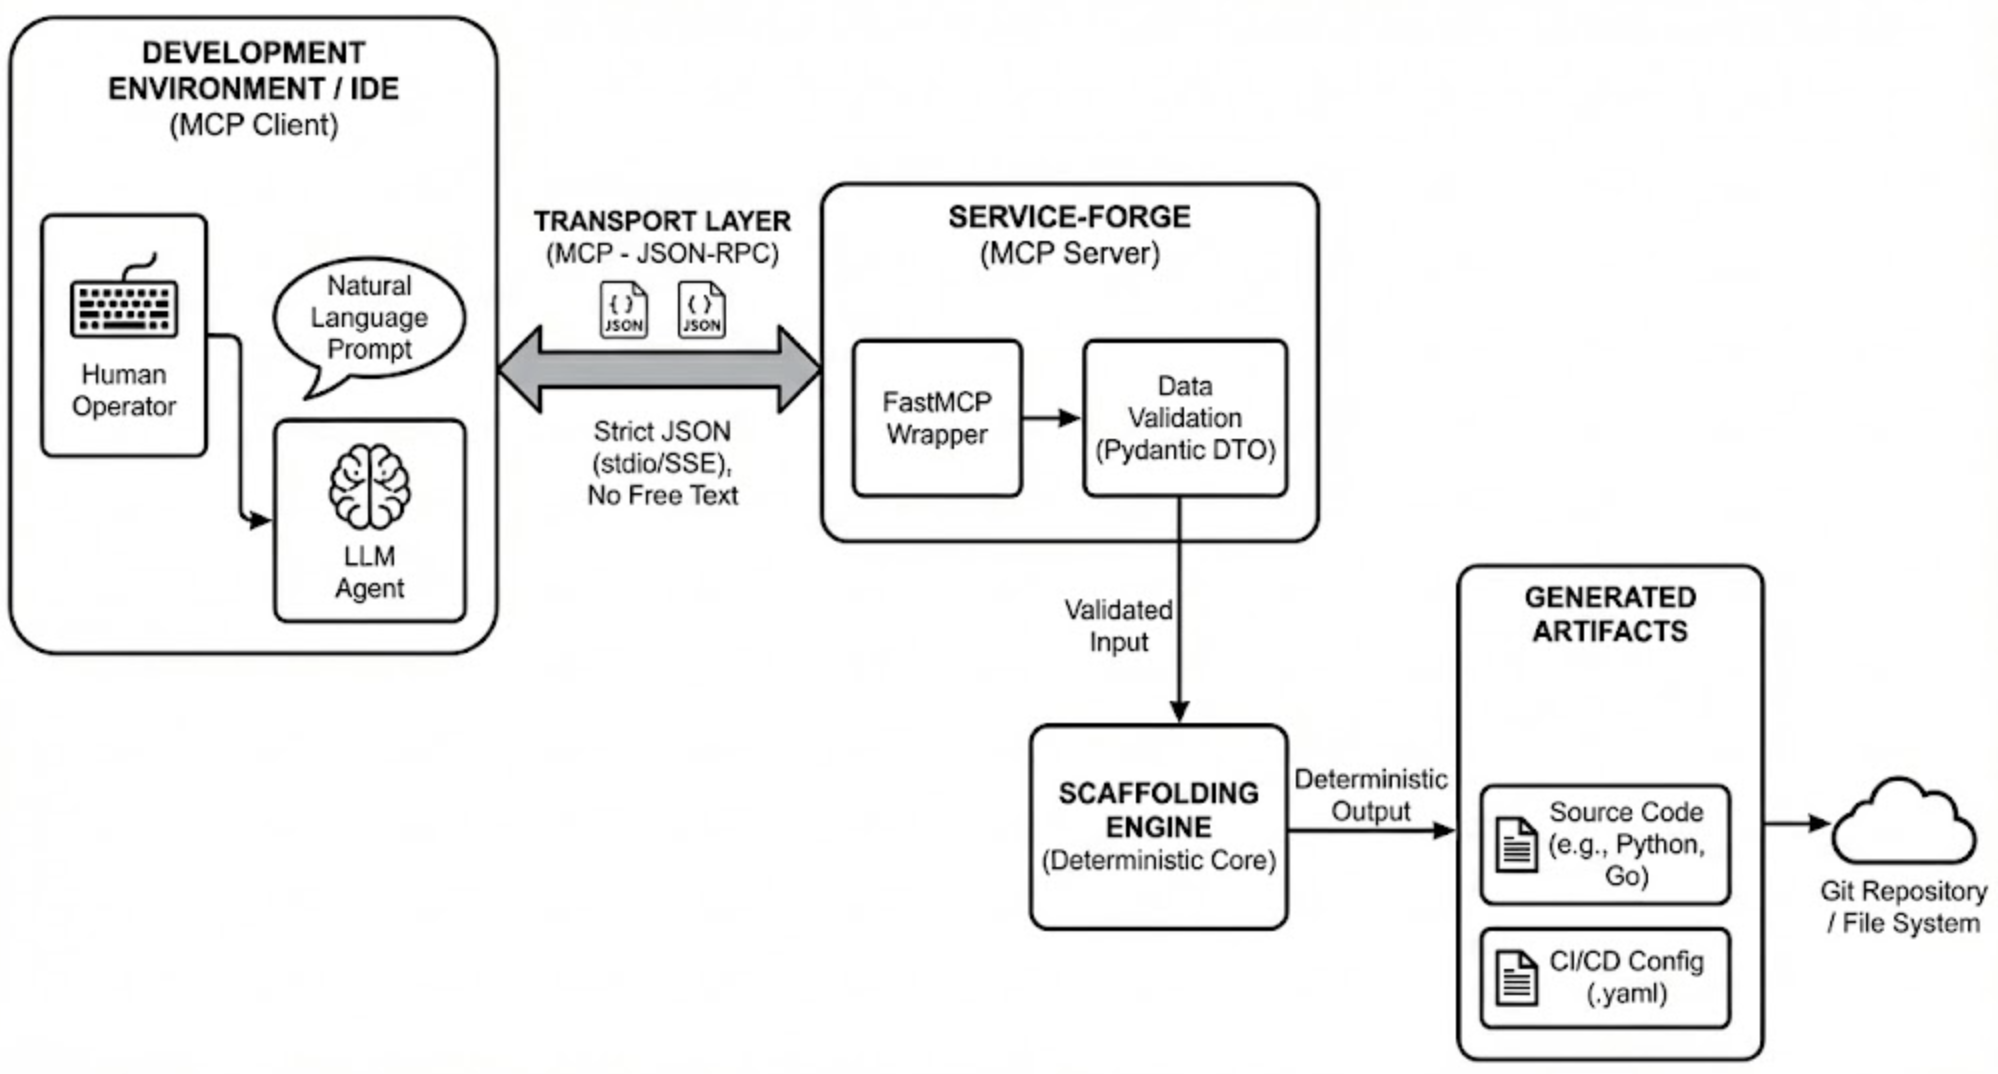
\includegraphics[width=1\textwidth]{images/mcp-architecture.png}
    \caption{Architettura logica dell'integrazione MCP. Il diagramma illustra la separazione delle responsabilità tra l'IDE (Client MCP) delegato all'estrazione semantica tramite LLM, e Service-Forge (Server MCP) responsabile della validazione Pydantic e dell'esecuzione deterministica dello scaffolding [Elaborazione dell'autore].}
    \label{fig:design_mcp_architecture}
\end{figure}

L'architettura delega all'Intelligenza Artificiale esclusivamente l'estrazione semantica dei parametri (es. il nome del servizio, il pattern architetturale desiderato) e la relativa formattazione in una struttura dati JSON valida, come illustrato nello schema di Figura \ref{fig:design_mcp_architecture}. Il nucleo deterministico del sistema (Service-Forge) riceve tale payload, lo sottopone a una rigorosa validazione sintattica tramite schemi Pydantic e, in caso di esito positivo, avvia l'esecuzione del codice di scaffolding.
Questo pattern di progettazione, comunemente noto come AI-Augmented Platform Engineering, confina la non-determinabilità dell'LLM all'interfaccia utente, mantenendo il controllo assoluto e deterministico sulla generazione degli artefatti software e infrastrutturali aziendali.

\chapter{Implementazione}
\label{chap:implementazione}

Questo capitolo descrive l'implementazione tecnica della soluzione architetturale progettata nel Capitolo \ref{chap:analisi}. La trattazione segue un approccio bottom-up, partendo dalla base infrastrutturale fino ad arrivare agli strumenti di automazione per gli sviluppatori.  La prima fase dell'implementazione riguarda la traduzione della topologia cloud in codice Terraform, necessaria per istanziare gli ambienti di base. Successivamente, il capitolo dettaglia la scrittura del codice applicativo, separando i processi asincroni del livello dati dall'implementazione delle API sincrone di backend. Una volta definiti i componenti cloud e applicativi, la trattazione si sposta sulle metodologie adottate per garantire la testabilità del codice sulla workstation dello sviluppatore tramite emulazione locale. Il consolidamento di questi processi culmina nell'implementazione delle pipeline di Continuous Integration e Continuous Deployment, che eliminano l'intervento manuale nei rilasci. Infine, illustra lo sviluppo di Service-Forge, il framework interno creato per automatizzare la generazione di nuovi microservizi interfacciando l'infrastruttura prodotta con agenti basati su Large Language Models.

\section{Provisioning dell'Infrastruttura tramite Terraform}

L'adozione di un approccio Infrastructure as Code (IaC) garantisce la riproducibilità, la tracciabilità e la coerenza degli ambienti cloud. Il repository oggetto di questa sezione traduce la topologia cloud, descritta nei capitoli precedenti, in codice HCL (HashiCorp Configuration Language), il linguaggio dichiarativo utilizzato da Terraform per definire risorse infrastrutturali. Ogni componente trova una corrispondenza diretta in moduli Terraform versionati e organizzati secondo una struttura gerarchica.

Come discusso nel Capitolo \ref{chap:analisi}, la scelta di Terraform come strumento di provisioning deriva da tre fattori tecnici: la natura dichiarativa del linguaggio, che delega al motore il calcolo del piano di esecuzione; il supporto multi-provider, essenziale per gestire risorse AWS, Google Cloud Platform e MongoDB Atlas in un singolo repository; e l'ecosistema di moduli riutilizzabili.

La gestione dello stato per ambienti multipli richiede l'utilizzo di Terragrunt come orchestratore. Terragrunt opera come wrapper per Terraform, aggiungendo funzionalità di gestione dello stato remoto, generazione automatica di file di configurazione e risoluzione delle dipendenze tra moduli \cite{Terragrunt}. Questa combinazione applica il principio Don't Repeat Yourself alla definizione dell'infrastruttura.

La struttura logica di questa sezione segue il flusso di astrazione dell'infrastruttura: la scomposizione iniziale del repository illustra la separazione tra configurazione e implementazione; le sezioni successive dettagliano l'orchestrazione dello stato, la segregazione degli ambienti (multi-account) e, infine, la logica interna dei moduli riutilizzabili sviluppati per la piattaforma.

\subsection{Struttura del Repository}

Il repository implementa una separazione netta tra tre livelli logici, come illustrato in Figura \ref{fig:architettura_repo_devops}: le configurazioni Terragrunt specifiche per ambiente (directory \texttt{infra/}), le definizioni delle risorse Terraform raggruppate per dominio funzionale (directory \texttt{resources/}) e i moduli riutilizzabili (directory \texttt{utils/modules/}).

\begin{lstlisting}[basicstyle=\ttfamily\small, breaklines=true, columns=fullflexible]
devops-farm-tf/
|-- infra/                          # Configurazioni Terragrunt
|   |-- root.hcl                    # Configurazione globale
|   |-- _env/                       # Template di modulo (env-agnostic)
|   |   |-- 000-commons.hcl
|   |   |-- 010-networkings.hcl
|   |   |-- 020-messaging.hcl
|   |   |-- 050-integrations.hcl
|   |   |-- 060-mongodb.hcl
|   |   |-- 070-microservices.hcl
|   |   +-- 090-dwh.hcl
|   |-- dev/                        # Ambiente di sviluppo
|   |   |-- env.hcl
|   |   |-- 000-commons/
|   |   |-- 010-networkings/
|   |   |-- 020-messaging/
|   |   |-- 070-microservices/
|   |   +-- ...
|   |-- prod/                       # Ambiente di produzione
|   +-- shared/                     # Account condiviso
|       |-- main/                   # Organizzazione AWS
|       +-- shared/                 # Risorse condivise (ECR, domini)
|
|-- resources/                      # Definizioni Terraform per dominio
|   |-- 000-commons/                # OIDC GitHub, API GCP, IAP
|   |-- 010-networkings/            # VPC, subnet, NAT Gateway
|   |-- 020-messaging/              # Topic SNS
|   |-- 050-integrations/           # Service account GCP
|   |-- 060-mongodb/                # Cluster MongoDB Atlas
|   |-- 070-microservices/          # Cognito, Lambda, ECS, S3, DynamoDB
|   |-- 090-dwh/                    # Athena, Glue, Data Warehouse
|   |-- main/                       # AWS Organizations, SSO, IAM
|   +-- shared/                     # ECR, domini Route53
|
+-- utils/modules/                  # Moduli Terraform riutilizzabili
    |-- api-gateway-lambda/         # API Gateway HTTP + Lambda + Cognito
    |-- datasource-etl/             # Pipeline ETL: Extr + Tran + Glue + Athena
    |-- scheduled-lambda/           # EventBridge + Lambda schedulata
    +-- sns-consumer-lambda/        # SNS -> Lambda consumer
\end{lstlisting}

La numerazione progressiva delle directory sotto \texttt{resources/} (es. 000, 010, 020) riflette rigorosamente l'ordine di applicazione delle risorse e le dipendenze logiche: le risorse di rete (010) precedono il deployment dei microservizi (070).

\begin{figure}[htbp]
    \centering
    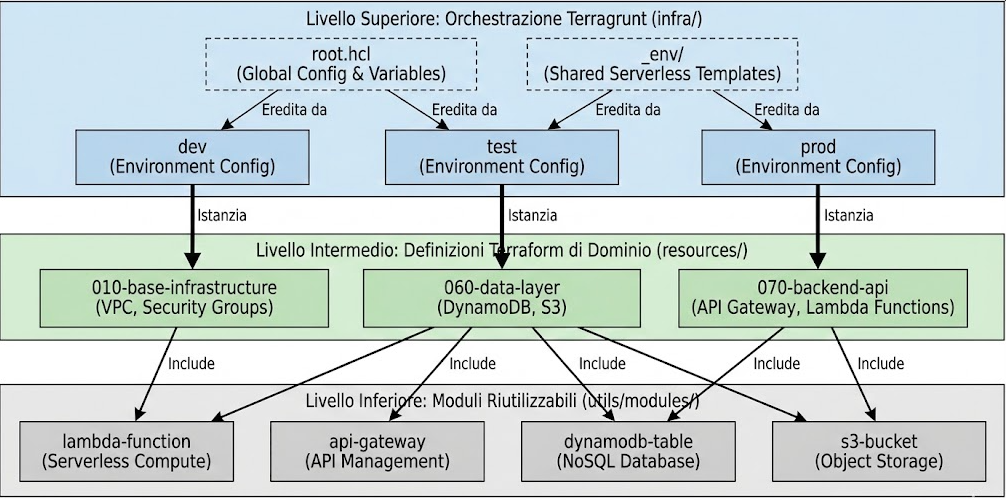
\includegraphics[width=1\textwidth]{images/architettura_repo_devops.png}
    \caption{Architettura logica del repository di Infrastructure as Code. Il diagramma illustra la gerarchia di orchestrazione tra le configurazioni di ambiente gestite tramite Terragrunt (livello superiore), le definizioni dei domini funzionali (livello intermedio) e i moduli Terraform di base riutilizzabili (livello inferiore) [Elaborazione dell'autore].}
    \label{fig:architettura_repo_devops}
\end{figure}

\subsection{Orchestrazione con Terragrunt}

Terragrunt introduce un livello di astrazione che risolve la configurazione del backend remoto, la generazione dei file provider e la gestione delle dipendenze tra moduli.

\subsubsection{Gestione dello Stato Remoto e Provider}

Lo stato di Terraform contiene la mappatura tra le risorse dichiarate nel codice e quelle allocate nel cloud. Per garantire persistenza, cifratura server-side e mutua esclusione durante le operazioni concorrenti, il repository utilizza un backend Amazon S3 con meccanismo di lock affidato ad Amazon DynamoDB.

Terragrunt genera automaticamente il file \texttt{provider.tf} per ogni modulo. La piattaforma richiede tre provider AWS distinti e un provider Google Cloud per gestire risorse eterogenee.

\subsubsection{Gerarchia di Inclusione e Dipendenze}

Ogni modulo in un ambiente specifico è rappresentato da un file \texttt{terragrunt.hcl} che combina la configurazione globale con il template del modulo e le dipendenze specifiche. Questa composizione a tre livelli (root, template, ambiente) centralizza la logica. Ad esempio, il blocco \texttt{dependency} consente di estrapolare gli output di un modulo già applicato (es. l'infrastruttura di messaggistica) e passarli come input al modulo corrente (es. i microservizi).

\subsection{Architettura Multi-Account}

La piattaforma opera su un'organizzazione AWS composta da ambienti segregati (dev, prod, shared), la cui topologia è schematizzata in Figura \ref{fig:aws_multi_account_topology}. L'utilizzo del servizio AWS Organizations permette di istanziare account separati, assegnando indirizzi email univoci e ruoli amministrativi per l'assunzione di identità cross-account.

L'accesso degli operatori è regolato tramite IAM Identity Center. Il modulo definisce gruppi e permission set specifici; ad esempio, il gruppo assegnato all'analisi dati riceve esclusivamente i permessi di lettura per interrogare il data warehouse tramite Amazon Athena, senza facoltà di modifica sulle risorse.

\subsection{Moduli Riutilizzabili}

La directory \texttt{utils/modules/} contiene i moduli Terraform che incapsulano i pattern architetturali ricorrenti.

\subsubsection{Modulo \texttt{api-gateway-lambda}}

Questo modulo rappresenta il pattern standard per il deployment dei microservizi serverless. Crea un endpoint HTTP (API Gateway v2), una funzione Lambda, un authorizer JWT \cite{JWT} opzionale basato su Amazon Cognito e i relativi gruppi di log in CloudWatch.

Un aspetto ingegneristico rilevante risiede nella separazione tra il ciclo di vita dell'infrastruttura e quello del codice applicativo. Nel blocco di definizione della funzione Lambda, l'attributo \texttt{image\_uri} viene escluso dal monitoraggio dello stato di Terraform:

\begin{lstlisting}[language=HCL]
resource "aws_lambda_function" "lambda" {
  function_name = "${var.name}-${var.env}"
  role          = aws_iam_role.lambda_assume_role.arn
  package_type  = "Image"
  image_uri     = var.app_image

  lifecycle {
    ignore_changes = [image_uri]
  }

  timeout       = var.lambda_timeout
  memory_size   = var.lambda_memory_size
  architectures = ["arm64"]

  environment {
    variables = merge(
      var.environments,
      {
        CLOUD_ENV = var.env
        STAGE     = "/api"
    })
  }
}
\end{lstlisting}

Questa direttiva impedisce a Terraform di ripristinare una versione precedente dell'immagine Docker qualora l'applicazione sia stata aggiornata in modo asincrono dalle pipeline di Continuous Deployment. La policy IAM della funzione viene costruita dinamicamente componendo i permessi di base (scrittura dei log) con istruzioni opzionali passate dal modulo chiamante, consentendo un'applicazione granulare del principio del minimo privilegio.

\subsubsection{Modulo \texttt{datasource-etl}}

Questo modulo definisce la pipeline ETL (Extract, Transform, Load) per l'ingestione dei dati. L'architettura di questo componente, dettagliata in Figura \ref{fig:pipeline-etl}, prevede una netta separazione fisica e logica dei dati: un prefisso S3 \texttt{raw/} per i dati grezzi e un prefisso \texttt{clean/} per i dati trasformati in formato Apache Parquet.

L'orchestrazione si divide in due fasi computazionali. La fase di estrazione (Extractor) utilizza una funzione Lambda invocata temporalmente tramite regole Amazon EventBridge. Per evitare la duplicazione dei dati grezzi in caso di errori temporanei della sorgente, i retry automatici dell'invocazione asincrona sono disabilitati (\texttt{maximum\_retry\_attempts = 0}).

La fase di trasformazione è puramente event-driven: viene attivata dalle notifiche S3 alla creazione di un nuovo oggetto nel prefisso \texttt{raw/}. Le policy IAM dei due componenti riflettono il flusso dei dati: l'Extractor ha permessi di sola scrittura su \texttt{raw/}, mentre il Transformer legge da \texttt{raw/} e scrive esclusivamente su \texttt{clean/}.

I dati elaborati vengono resi interrogabili tramite l'integrazione con AWS Glue Catalog e Amazon Athena. Il modulo implementa la funzionalità di Partition Projection per ottimizzare le query; le partizioni temporali (anno, mese, giorno) vengono calcolate matematicamente dal motore di Athena in base a range predefiniti, eliminando la necessità di eseguire operazioni di scansione sincrona (crawler) sui bucket S3.

\subsection{Risorse Condivise e Continuous Integration}

L'account condiviso ospita i repository Elastic Container Registry (ECR). L'accesso da parte dei sistemi di Continuous Integration (GitHub Actions) avviene senza lo scambio di credenziali, sfruttando il protocollo OIDC (OpenID Connect). Il provider di identità assume un ruolo IAM temporaneo che garantisce unicamente i permessi di push sui repository di destinazione.

\subsection{Strategia di Tagging}

Ogni risorsa gestita tramite IaC riceve un set di tag obbligatori (\texttt{terraform}, \texttt{environment}, \texttt{project}, \texttt{subproject}). Oltre all'identificazione visiva, questi metadati sono integrati con AWS Cost Explorer come Cost Allocation Tags, permettendo l'analisi e la ripartizione dei costi infrastrutturali per specifico dominio funzionale o ambiente.

\section{Sviluppo del Flusso ETL Event-Driven}
\label{sec:sviluppo-flusso-etl}
Questa sezione dettaglia l'implementazione applicativa della pipeline di ingestione dati. L'analisi procede seguendo il ciclo di vita dell'evento asincrono: l'inizializzazione e validazione del payload di estrazione, l'instradamento dinamico verso i moduli di integrazione esterni e, infine, la trasformazione del dato in memoria con conseguente serializzazione nel formato colonnare Parquet. La logica software è progettata per operare all'interno dei limiti computazionali ed effimeri del runtime serverless descritto nel Capitolo \ref{chap:analisi}.

\subsection{Logica Applicativa di Estrazione}

L'estrattore ETL opera come un componente senza stato che interroga una sorgente esterna per produrre dati grezzi in risposta a un evento asincrono. Per standardizzare lo sviluppo ed evitare la duplicazione del codice tra i vari microservizi, il sistema integra un repository condiviso importato come submodule Git \cite{Submodules}. Questo modulo isola il codice infrastrutturale di base, offrendo un livello di astrazione per l'interazione con le risorse cloud e permettendo all'estrattore di concentrarsi unicamente sulla logica di recupero dati.

L'innesco del processo avviene tramite un payload JSON strutturato, il quale definisce il contesto dell'operazione. Il contratto dei dati prevede quattro parametri essenziali: l'identificativo del servizio da interrogare (\texttt{service}), la finestra temporale dell'estrazione, una chiave di partizionamento (\texttt{iterator}) per supportare esecuzioni parallele in ambienti multi-tenant, e i metadati per il tracciamento distribuito.

La validazione a runtime del payload è demandata alla libreria Pydantic. L'istanziamento rigoroso del modello dati, mostrato nel Listato \ref{lst:extractor-input}, implementa un meccanismo di interruzione rapida (fail-fast): il sistema scarta istantaneamente le richieste malformate prima di allocare risorse o inizializzare connessioni di rete verso i provider esterni.

\begin{lstlisting}[language=Python,caption={Modello Pydantic per la validazione formale del payload in ingresso},label={lst:extractor-input}]
from pydantic import BaseModel, Field
from datetime import datetime

class ExtractorInput(BaseModel):
    service: str = Field(..., description="Identificativo del servizio da interrogare")
    start_date: datetime
    end_date: datetime
    iterator: int = Field(..., description="Chiave di partizionamento")
    application_name: str
\end{lstlisting}

Il controllo del flusso interno all'estrattore impiega un meccanismo di instradamento basato sul parametro \texttt{service}. Per rispettare il principio Open/Closed e garantire l'estensibilità della piattaforma, l'architettura adotta il pattern architetturale Registry. Questo schema, illustrato nel Listato \ref{lst:registry-pattern}, mappa in modo statico ogni servizio esterno alla propria funzione di estrazione dedicata, eliminando la necessità di costrutti condizionali centralizzati (anti-pattern spesso riscontrabile in architetture monolitiche).

\begin{lstlisting}[language=Python,caption={Implementazione del pattern Registry per l'instradamento disaccoppiato dei servizi},label={lst:registry-pattern}]
from typing import Callable, Dict

class ServiceRegistry:
_registry: Dict[str, Callable] = {}

@classmethod
def register(cls, service_name: str) -> Callable:
    def decorator(func: Callable):
        cls._registry[service_name] = func
        return func
    return decorator

@classmethod
def get_handler(cls, service_name: str) -> Callable:
    handler = cls._registry.get(service_name)
    if not handler:
        raise ValueError(f"Nessun handler per: {service_name}")
    return handler
\end{lstlisting}

L'aggiunta di una nuova sorgente dati risulta perciò un'operazione circoscritta: l'ingegnere implementa la specifica logica di chiamata HTTP e la annota con il decoratore \texttt{\@ServiceRegistry.register("nome\_servizio")}. L'applicativo carica questi moduli dinamicamente durante la fase di avvio del runtime (cold start), abilitando un comportamento strettamente modulare.

La robustezza dell'estrattore è garantita da ulteriori decoratori applicativi, sviluppati per uniformare la gestione delle anomalie di rete. Il sistema classifica le eccezioni in errori temporanei (es. \emph{rate limit}, latenze del server remoto), che giustificano un successivo ritentativo, ed errori fatali (es. permessi mancanti), che interrompono definitivamente l'esecuzione. Il Listato \ref{lst:handle-etl-errors} mostra come il decoratore isoli l'esecuzione del gestore, traducendo le eccezioni generiche in classi di errore di dominio per il corretto instradamento verso l'infrastruttura di scarto (Dead Letter Queue).

\begin{lstlisting}[language=Python,caption={Decoratore per la classificazione e gestione uniforme degli errori di rete},label={lst:handle-etl-errors}]
import functools
import re

DEFAULT_RETRYABLE = [r"rate limit", r"502", r"QUOTA"]

class EtlRetryableError(Exception): pass
class EtlFatalError(Exception): pass

def handle_etl_errors(func):
@functools.wraps(func)
def wrapper(*args, **kwargs):
    try:
        return func(*args, **kwargs)
    except Exception as e:
        if any(re.search(p, str(e), re.I) for p in DEFAULT_RETRYABLE):
            raise EtlRetryableError(f"{func.name}: {e}") from e
        raise EtlFatalError(f"{func.name}: {e}") from e
    return wrapper
\end{lstlisting}

Al termine dell'elaborazione in memoria, l'estrattore finalizza il processo confinando il payload grezzo ottenuto nel livello di archiviazione persistente. L'estrattore salva il file all'interno del prefisso \texttt{raw/} del bucket di destinazione, utilizzando una chiave deterministica contenente il nome del servizio utilizzato per l'estrazione basata sui parametri del payload originale. Una volta confermata la scrittura remota, la funzione termina l'esecuzione, concludendo il ciclo vitale del worker e innescando, a livello infrastrutturale, l'evento per la successiva fase di trasformazione.


\subsection{Trasformazione del Dato e Serializzazione in Parquet}

Il componente di trasformazione esegue l'elaborazione dei dati grezzi estratti nella fase precedente. L'inserimento di un nuovo file nel percorso \texttt{raw/} del bucket Amazon S3 genera un evento asincrono che innesca automaticamente l'esecuzione della funzione AWS Lambda. L'handler della funzione intercetta il payload dell'evento, estrae la chiave identificativa dell'oggetto S3 e procede al download del file grezzo nell'ambiente di esecuzione temporaneo (\texttt{/tmp}). Una volta caricato in memoria, il software applica le logiche di pulizia, valida lo schema dei dati e serializza le informazioni nel formato colonnare Parquet, archiviando infine il risultato nel percorso \texttt{clean/} del Data Lake.

L'adozione della libreria Python Polars \cite{Polars} per la manipolazione dei dati in memoria è motivata da tre fattori principali. Il primo fattore riguarda l'efficienza delle operazioni di I/O: l'utilizzo di un motore di esecuzione interno ottimizzato riduce la pressione sulla memoria allocata, mitigando le restrizioni intrinseche ai runtime effimeri come AWS Lambda. Il secondo fattore concerne la tipizzazione esplicita: Polars applica un cast rigoroso verso tipi di dato primitivi (quali interi a 64 bit o timestamp), uniformando in modo deterministico le discrepanze presenti nei set di dati JSON in ingresso. Il terzo fattore è la disponibilità di trasformazioni vettoriali, le quali permettono di eseguire operazioni di validazione e manipolazione su intere colonne simultaneamente, ottimizzando i tempi di esecuzione rispetto a un'iterazione procedurale.

\begin{lstlisting}[language=Python,caption={Estrazione della chiave dall'evento S3 e caricamento del file JSON in un DataFrame Polars},label={lst:s3-extract}]
from urllib.parse import unquote_plus
import polars as pl
import os

def get_path_from_event(event: dict) -> str:
    record = event["Records"][0]
    return unquote_plus(record["s3"]["object"]["key"])

def read_s3_file(s3_client, key: str) -> pl.DataFrame:
    local_path = f"/tmp/{os.path.basename(key)}"
    s3_client.download_file(key, local_path)
    return pl.read_json(local_path)
\end{lstlisting}

Per orchestrare le molteplici varianti strutturali dei formati in ingresso, l'architettura implementa un costrutto logico che combina il pattern Factory con un registro statico. Ogni classe concreta, dedicata a una specifica strategia di trasformazione, dichiara la propria registrazione tramite un decoratore sintattico, associandosi a una stringa identificativa univoca. Durante l'elaborazione, il sistema ispeziona la configurazione per estrarre la chiave di instradamento e istanzia dinamicamente la classe corretta. Questo design, illustrato nel Listato \ref{lst:factory-registry}, separa il contratto di base dalle implementazioni specifiche di dominio, eliminando i costrutti condizionali monolitici e agevolando l'estensione del codice.

\begin{lstlisting}[language=Python,caption={Registrazione delle strategie di trasformazione e risoluzione dinamica tramite pattern Factory},label={lst:factory-registry}]
from typing import Type, Dict

STRATEGY_REGISTRY: Dict[str, Type] = {}

def register_strategy(strategy_name: str):
    def decorator(cls):
        if strategy_name in STRATEGY_REGISTRY:
            raise ValueError(f"Strategia '{strategy_name}' gia' registrata")
        STRATEGY_REGISTRY[strategy_name] = cls
        return cls
    return decorator

def create_transformer(config_key: str, payload: dict):
    strategy_name = get_strategy_from_config(config_key)
    transformer_cls = STRATEGY_REGISTRY.get(strategy_name)
    if not transformer_cls:
        raise ValueError(f"Strategia '{strategy_name}' non trovata")
    return transformer_cls(payload)
\end{lstlisting}

Il processo di sanificazione dei dati si articola su due livelli logici distinti. Il primo livello, incapsulato all'interno della classe astratta di base, applica le regole di validazione comuni a tutti i flussi operativi. La classe base esegue la rimozione degli spazi bianchi superflui (trimming) su tutte le stringhe e normalizza i token testuali anomali, convertendoli nel tipo nullo nativo del linguaggio. Il codice gestisce inoltre l'adeguamento delle unità di misura, come la conversione di valori finanziari in micro-unità tramite divisione scalare, e forza la standardizzazione dei formati temporali.

Il secondo livello di sanificazione è demandato ai trasformatori concreti, i quali gestiscono le difformità strutturali di specifici set di dati. A titolo esemplificativo, le classi specializzate eseguono la fusione di colonne separate per data e ora in un singolo timestamp, oppure applicano operazioni di \emph{flattening} per convertire le strutture nidificate dei documenti JSON in schemi tabellari piatti. Al termine di questi processi di pulizia, il trasformatore formatta il DataFrame risultante in Parquet e il client delegato lo trasferisce definitivamente nella directory \texttt{clean/} del bucket S3, predisponendo i dati per l'interrogazione analitica.

\subsection{Interrogazione Analitica e Viste Materializzate in Athena}

Il livello analitico del sistema si fonda su Amazon Athena e implementa una duplice strategia di interrogazione e strutturazione dei dati. La prima operazione consiste nella materializzazione fisica dei risultati all'interno del livello di archiviazione. Il processo impiega l'istruzione SQL \texttt{UNLOAD} per generare e depositare i dataset analitici direttamente su Amazon S3. L'operazione serializza i dati in Parquet e applica l'algoritmo di compressione Snappy \cite{Snappy}, organizzando i file fisici secondo una gerarchia di directory basata sulle partizioni temporali (anno, mese, giorno).

\begin{lstlisting}[language=SQL, caption={Materializzazione dei risultati partizionati tramite UNLOAD in fase di esecuzione ETL}, label={lst:athena-unload}]
UNLOAD (
    SELECT *
    FROM <table_name>_raw
    WHERE date_parse(year || '-' || month || '-' || day, '%Y-%m-%d')
        BETWEEN DATE '<date_start>' AND DATE '<date_end>'
        AND iterator = '<iterator>'
)
TO 's3://<bucket>/athena-results/<table_name>/year=<YYYY>/month=<MM>/day=<DD>/'
WITH (
    format = 'PARQUET', 
    compression = 'SNAPPY'
);
\end{lstlisting}

La seconda operazione analitica riguarda l'accesso trasparente ai dati in continua mutazione. L'architettura adotta un pattern organizzativo che separa i dati recenti (volatili o di \emph{staging}) dai dati storici consolidati (identificati come \emph{freeze}). Per fornire un singolo punto di accesso logico alle applicazioni a valle, l'infrastruttura istanzia una vista virtuale unificata. Tale costrutto relazionale impiega l'operatore \texttt{UNION ALL} per concatenare dinamicamente le due tabelle sottostanti, schermando la complessità strutturale ai consumatori finali.

\begin{lstlisting}[language=SQL, caption={Dichiarazione DDL per la creazione della vista unificata staging e freeze}, label={lst:athena-unified-view}]
CREATE OR REPLACE VIEW daily_creatives_delivery_unified_view AS
    SELECT * FROM daily_creatives_delivery_staging
    UNION ALL
    SELECT * FROM daily_creatives_delivery_freeze;
\end{lstlisting}

L'estrazione delle metriche di business richiede interrogazioni di aggregazione strutturate. Una delle operazioni principali riguarda il monitoraggio dell'erogazione giornaliera delle creatività pubblicitarie. Il motore Athena esegue un'interrogazione che aggrega le impressioni e i clic generati, escludendo a priori il traffico attribuibile a sistemi automatizzati (\texttt{$is\_robot = false$}). Il costrutto logico utilizza le \emph{Common Table Expressions} (CTE) per pre-calcolare le metriche sulle tabelle dei fatti, eseguendo successivamente un'operazione di \texttt{LEFT JOIN} con le tabelle dimensionali contenenti i metadati delle campagne e dei posizionamenti.

\begin{lstlisting}[language=SQL, caption={Interrogazione analitica con CTE per l'aggregazione delle metriche di erogazione giornaliera}, label={lst:athena-daily-creatives}]
WITH imps AS (
    SELECT
        i.year,
        i.month,
        i.day,
        campaign_id,
        placement_id_activity_id,
        banner_id_ad_group_id,
        COUNT(*) AS impression,
        SUM(rtb_cost) AS rtb_cost
    FROM "adform-prod"."impression" AS i
    WHERE is_robot = false
    GROUP BY 1, 2, 3, 4, 5, 6
),
cls AS (
    SELECT
        c.year,
        c.month,
        c.day,
        campaign_id,
        placement_id_activity_id,
        banner_id_ad_group_id,
        COUNT(*) AS click
    FROM "adform-prod"."click" AS c
    WHERE is_robot = false
    GROUP BY 1, 2, 3, 4, 5, 6
)
SELECT
    DATE(i.year || '-' || i.month || '-' || i.day) AS date,
    c.name AS campaign,
    p.name AS line_item,
    b.name AS creative,
    i.impression,
    COALESCE(cls.click, 0) AS click,
    i.rtb_cost AS cost
FROM imps i
LEFT JOIN cls
    ON  i.year = cls.year
    AND i.month = cls.month
    AND i.day = cls.day
    AND i.campaign_id = cls.campaign_id
    AND i.placement_id_activity_id = cls.placement_id_activity_id
    AND i.banner_id_ad_group_id = cls.banner_id_ad_group_id
LEFT JOIN "adform-prod"."campaigns" c
    ON c.id = i.campaign_id
LEFT JOIN "adform-prod"."placements_activities" p
    ON p.id = i.placement_id_activity_id
LEFT JOIN "adform-prod"."banners_adgroups" b
    ON b.id = i.banner_id_ad_group_id;
\end{lstlisting}

Il calcolo del Click-Through Rate (CTR) esemplifica l'efficacia del partizionamento dei dati. La metrica è definita come il rapporto percentuale tra i clic ricevuti e le impressioni erogate:

\begin{equation}
\text{CTR} (\%) = \frac{\text{click}}{\text{impression}} \times 100
\label{eq:ctr_formula}
\end{equation}

L'estrazione di questo valore impone l'applicazione di filtri espliciti sulle colonne di partizionamento temporale. La dichiarazione esplicita dell'anno e del mese all'interno della clausola \texttt{WHERE} istruisce il motore di esecuzione a ignorare i dati non pertinenti alla finestra temporale analizzata.

\begin{lstlisting}[language=SQL, caption={Estrazione del KPI con applicazione dei predicati di partizionamento temporale}, label={lst:athena-ctr}]
WITH imp AS (
    SELECT
        campaign_id,
        COUNT(*) AS impressions
    FROM "adform-prod"."impression"
    WHERE is_robot = false
        AND year = '2024'
        AND month = '02'
    GROUP BY campaign_id
),
clk AS (
    SELECT
        campaign_id,
        COUNT(*) AS clicks
    FROM "adform-prod"."click"
    WHERE is_robot = false
        AND year = '2024'
        AND month = '02'
    GROUP BY campaign_id
)
SELECT
    i.campaign_id,
    i.impressions,
    COALESCE(c.clicks, 0) AS clicks,
    100.0 * COALESCE(c.clicks, 0) / NULLIF(i.impressions, 0) AS ctr_pct
FROM imp i
LEFT JOIN clk c
    ON c.campaign_id = i.campaign_id
ORDER BY ctr_pct DESC;
\end{lstlisting}

L'implementazione di questo modello architetturale comporta quattro conseguenze dirette. In primo luogo, la combinazione del formato colonnare Parquet con la compressione Snappy ottimizza i tempi di caricamento e i costi di I/O. In secondo luogo, la clausola \texttt{WHERE} applicata alle partizioni temporali limita il volume di dati scansionati dal motore serverless per singola query. Il terzo aspetto riguarda la governabilità, garantita dalla segregazione logica tra le elaborazioni recenti e l'archivio storico. Infine, la definizione della vista unificata fornisce un'interfaccia stabile e disaccoppiata per i sistemi di visualizzazione e i cruscotti analitici a valle.

\section{Implementazione dei Servizi Backend}
\label{sec:implementazione-backend}

Questa sezione analizza l'implementazione del livello applicativo sincrono, strutturata seguendo il ciclo di vita di una richiesta HTTP. L'analisi parte dal livello di instradamento, dove le richieste vengono intercettate e validate tramite iniezione delle dipendenze; prosegue illustrando il \emph{wrapper} necessario all'esecuzione del framework all'interno del runtime serverless; e si conclude nel livello di persistenza, descrivendo la mappatura a oggetti per il database NoSQL e la gestione della coerenza transazionale distribuita.

\subsection{Iniezione delle dipendenze e validazione tramite Pydantic}

L'architettura dei servizi di backend sfrutta il pattern \emph{Dependency Injection} per disaccoppiare la logica di business dalla risoluzione dei componenti tecnici e dalle precondizioni di dominio. Questo approccio, nativamente supportato da FastAPI, permette al sistema di eseguire controlli preliminari, quali la verifica dell'esistenza di una risorsa, l'autenticazione o il blocco di inserimenti duplicati, prima che la richiesta raggiunga il gestore principale.

\begin{lstlisting}[language=Python, caption={Esempio di iniezione delle dipendenze per la validazione semantica a livello di instradamento}, label={lst:dependency-injection}]
@router.post("/", response_model=EntityResponse, status_code=status.HTTP_202_ACCEPTED)
def create_resource(
    payload: EntityCreateRequest = Depends(),
    storage_client = Depends(get_storage_client),
    parent_entity: BaseModel = Depends(ensure_entity_does_not_exist),
    user = Depends(get_authenticated_user)
):
    """
    Gestore della creazione risorsa con dipendenze pre-validate.
    """
    return process_resource_creation(parent_entity, storage_client, payload, user)
\end{lstlisting}

Per la validazione strutturale del payload, il framework impiega la libreria Pydantic. Il processo di convalida estende il controllo statico dei tipi, integrando trasformazioni dei dati e vincoli semantici direttamente nella definizione del modello. 

\begin{lstlisting}[language=Python, caption={Validazione avanzata e trasformazione dei dati tramite i validatori di modello Pydantic}, label={lst:pydantic-validation}]
from pydantic import BaseModel, model_validator
import re
import unicodedata

class BaseEntityModel(BaseModel):
    name: str

    @model_validator(mode="before")
    @classmethod
    def normalize_identifier(cls, data):
        if not isinstance(data, dict):
            return data
        
        name = data.get("name")
        if name:
            # Normalizzazione Unicode e rimozione spazi
            normalized = unicodedata.normalize('NFC', name).casefold().strip()
            # Sostituzione spazi con underscore per slug/ID
            data['normalized_name'] = re.sub(r'\s+', '_', normalized)
        return data
\end{lstlisting}

\subsection{Adattamento del runtime FastAPI su AWS Lambda}

L'esposizione di interfacce API sincrone tramite AWS Lambda e API Gateway impone un disaccoppiamento dei protocolli. L'implementazione utilizza l'adattatore \texttt{Mangum} per operare questa traduzione (da evento Lambda a standard ASGI) all'interno del codice sorgente.

\begin{lstlisting}[language=Python, caption={Involucro dell'applicazione FastAPI tramite l'adattatore Mangum per l'esecuzione serverless}, label={lst:mangum-adapter}]
from fastapi import FastAPI
from mangum import Mangum
from api.routers import primary_router, secondary_router

app = FastAPI(title="Backend Service API")

# Inclusione dei router divisionali
app.include_router(primary_router.router, prefix="/v1/primary")
app.include_router(secondary_router.router, prefix="/v1/secondary")

# Handler per convertire l'evento API Gateway in richiesta ASGI
lambda_handler = Mangum(app)
\end{lstlisting}

\subsection{Interazione con DynamoDB e Single Table Design in codice}

Il livello di persistenza interagisce con Amazon DynamoDB applicando il pattern Single Table Design. Il sistema memorizza entità eterogenee all'interno di un'unica tabella fisica, impiegando chiavi primarie logiche e composite per definire i percorsi di accesso. Per l'interazione con il database, l'architettura adotta la libreria PynamoDB \cite{Pynamodb} in sostituzione del client standard \texttt{boto3}. Questa scelta ingegneristica permette di astrarre le chiamate di rete a basso livello e fornisce un Object-Document Mapper (ODM) per l'ecosistema Python. L'implementazione governa il polimorfismo applicativo definendo una classe base astratta e molteplici sottoclassi specializzate, distinte da un attributo discriminatore gestito direttamente in modo dichiarativo dalla libreria.

\begin{lstlisting}[language=Python, caption={Definizione dei modelli ODM in PynamoDB per l'implementazione del Single Table Design e del polimorfismo}, label={lst:dynamodb-odm}]
from pynamodb.models import Model
from pynamodb.attributes import UnicodeAttribute, NumberAttribute
import os

class BaseEntityModel(Model):
    class Meta:
        table_name = os.environ.get("DYNAMODB_TABLE")
        region = os.environ.get("AWS_REGION", "eu-west-1")
    
    normalized_name = UnicodeAttribute(hash_key=True)
    entity_type = UnicodeAttribute(range_key=True)

class SpecificEntityModel(BaseEntityModel, discriminator='specific_type'):
    external_provider_id = UnicodeAttribute()
    configuration_flags = NumberAttribute(default=0)
\end{lstlisting}

Per supportare schemi di interrogazione complessi senza eseguire scansioni sequenziali dispendiose, lo schema dati include Indici Secondari Globali (GSI) specializzati. Il sistema definisce un indice dedicato all'impaginazione temporale globale e un indice sparso progettato per localizzare rapidamente i record tramite identificatori generati da sistemi di terze parti.

Infine, per garantire la coerenza transazionale durante la creazione di risorse che richiedono la comunicazione con servizi esterni, la logica applicativa utilizza un pattern di prenotazione (reservation pattern). Il microservizio effettua una scrittura condizionata su DynamoDB, inserendo un record con uno stato provvisorio. Successivamente, invoca l'API del provider esterno. In caso di risposta positiva, il sistema aggiorna l'elemento con l'identificativo definitivo; in caso di fallimento della chiamata di rete, l'applicativo esegue un rollback eliminando il record provvisorio e restituendo un codice di errore HTTP al client.

\subsection{Emulazione delle Risorse AWS tramite LocalStack}

Per simulare l'infrastruttura cloud senza richiedere connettività di rete o incorrere in costi di fatturazione, l'ambiente di sviluppo esegue l'applicativo LocalStack \cite{LocalStackPaper} all'interno di un container dedicato. Questo strumento espone un singolo endpoint di rete locale in grado di emulare le API di molteplici servizi AWS, tra cui Amazon DynamoDB, Amazon S3 e Amazon SNS. 

I microservizi applicativi reindirizzano il traffico verso le risorse simulate decodificando specifiche variabili d'ambiente. Come mostrato nel Listato \ref{lst:docker-compose-localstack}, la configurazione inietta l'URL dell'emulatore (\texttt{AWS\_ENDPOINT\_URL}) e credenziali crittografiche fittizie. Questo pattern di progettazione mantiene inalterata la semantica del codice sorgente, istruendo l'SDK (Boto3) del fornitore cloud senza richiederne la modifica.

\begin{lstlisting}[caption={Configurazione Docker Compose per l'iniezione delle variabili d'ambiente e l'avvio di LocalStack}, label={lst:docker-compose-localstack}]
services:
  task:
    environment:
      AWS_ENDPOINT_URL: http://localstack:4566
      AWS_ACCESS_KEY_ID: test
      AWS_SECRET_ACCESS_KEY: test
      AWS_DEFAULT_REGION: eu-west-1
      DYNAMODB_TABLE: proximity-campaign
      S3_BUCKET_NAME: proximity-campaign

  localstack:
    image: localstack/localstack:latest
    ports:
      - "4566:4566"
    volumes:
      - "./init-aws.sh:/etc/localstack/init/ready.d/init-aws.sh:ro"
\end{lstlisting}

Il demone Docker orchestra l'inizializzazione dell'ambiente emulato eseguendo uno script shell (\texttt{init-aws.sh}) montato come volume di sola lettura. Questo script provvede a istanziare le risorse cloud effimere e a popolare le basi di dati con le informazioni necessarie per il collaudo al momento dell'avvio. 

Un'operazione fondamentale riguarda la generazione delle tabelle DynamoDB per i servizi backend. Il comando di inizializzazione, esposto nel Listato \ref{lst:localstack-dynamodb-init}, dichiara esplicitamente lo schema delle chiavi primarie e alloca gli Indici Secondari Globali (GSI) necessari per supportare i medesimi pattern di accesso definiti nell'ambiente di produzione.

\begin{lstlisting}[language=bash, caption={Script bash di avvio per la creazione automatizzata della tabella DynamoDB emulata}, label={lst:localstack-dynamodb-init}]
awslocal dynamodb create-table \
    --table-name proximity-campaign \
    --attribute-definitions \
        AttributeName=normalized_campaign_name,AttributeType=S \
        AttributeName=type_bucket,AttributeType=S \
        AttributeName=created_at,AttributeType=S \
        AttributeName=adsquare_config_id,AttributeType=S \
    --key-schema \
        AttributeName=normalized_campaign_name,KeyType=HASH \
    --global-secondary-indexes '[
        {
            "IndexName": "timeline-index",
            "KeySchema": [
                {"AttributeName": "type_bucket", "KeyType": "HASH"},
                {"AttributeName": "created_at", "KeyType": "RANGE"}
            ],
            "Projection": {"ProjectionType": "ALL"},
            "ProvisionedThroughput": {"ReadCapacityUnits": 5, "WriteCapacityUnits": 5}
        },
        {
            "IndexName": "adsquare-config-index",
            "KeySchema": [
                {"AttributeName": "adsquare_config_id", "KeyType": "HASH"}
            ],
            "Projection": {"ProjectionType": "ALL"},
            "ProvisionedThroughput": {"ReadCapacityUnits": 5, "WriteCapacityUnits": 5}
        }
    ]'
\end{lstlisting}

Lo script assolve a una seconda funzione critica per il collaudo dei worker asincroni (pipeline ETL). Il codice provvede a caricare i file JSON di test all'interno dei bucket S3 emulati, replicando l'esatta gerarchia dei percorsi (\texttt{raw/}) attesa in produzione. Questa pre-inizializzazione dello stato consente di validare la logica di estrazione, la sanificazione e la trasformazione nel formato Parquet operando esclusivamente sulla memoria e sul disco locale.

Questa configurazione architetturale genera un ambiente di sviluppo locale isomorfo all'infrastruttura di destinazione. L'isolamento delle dipendenze garantisce un ciclo di collaudo deterministico e un riscontro immediato su eventuali difetti logici, riducendo il tempo necessario per le iterazioni di sviluppo prima del rilascio in ambiente cloud.

\section{Automazione del Rilascio e Pipeline GitOps (CI/CD)}
\label{sec:cicd}

Questa sezione illustra la topologia dell'infrastruttura di \emph{Continuous Integration} e \emph{Continuous Delivery} (CI/CD) implementata per il ciclo di vita del software. L'analisi procede separando logicamente tre fasi: la compilazione automatizzata e il versionamento semantico (CI), il meccanismo di promozione controllata verso gli ambienti di esecuzione (CD) e, infine, l'imposizione formale delle policy di sicurezza e \emph{rollback}.

\subsection{Versionamento Semantico e Compilazione (CI)}

L'architettura adotta un modello di distribuzione basato su release. Il processo determina il versionamento semantico analizzando la cronologia dei commit e innesca la compilazione dell'artefatto esclusivamente al momento della generazione effettiva di una nuova release. Il sistema di automazione esegue il job di compilazione e caricamento dell'immagine Docker solo se l'indicatore booleano conferma l'avvenuta creazione della release.

\begin{lstlisting}[caption={Definizione del job GitHub Actions di compilazione condizionato alla creazione della release}, label={lst:gha-release-build}]
on:
  push:
    branches: [main, master]

jobs:
  build:
    runs-on: ubuntu-latest
    steps:
      - uses: devredops/cicd-release-action@main
        id: release

      - name: Build and Push Docker Image to ECR
        if: ${{ steps.release.outputs.release-created }}
        uses: Company/gha-build-and-push-on-ecr@main
        with:
          ecr-repository: ${{ env.REPO_NAME }}
          release-version: ${{ steps.release.outputs.release-version }}
\end{lstlisting}

\subsection{Pipeline GitOps e Promotion Gate (CD)}

Al termine della compilazione e del push dell'immagine Docker sul registro Amazon ECR, il sistema interrompe l'esecuzione automatizzata. La distribuzione (\emph{deployment}) richiede un innesco esplicito tramite l'evento \texttt{workflow\_dispatch}, che introduce un \emph{promotion gate}.

\begin{lstlisting}[caption={Configurazione del trigger manuale per la promozione controllata degli artefatti nei vari ambienti}, label={lst:gha-promotion-gate}]
on:
  workflow_dispatch:
    inputs:
      environment:
        type: choice
        description: 'Ambiente di destinazione'
        options: [dev, prod]

jobs:
  deploy:
    runs-on: ubuntu-latest
    steps:
      - name: Update Lambda Image (Dev)
        if: github.event.inputs.environment == 'dev'
        uses: Company/gha-lambda-image-upload@main
        with:
          image-tag: ${{ env.RELEASE_VERSION }}

      - name: Update Lambda Image (Prod)
        if: github.event.inputs.environment == 'prod'
        uses: Company/gha-lambda-image-upload@main
        with:
          image-tag: ${{ env.RELEASE_VERSION }}
\end{lstlisting}

L'azione composita responsabile del caricamento incapsula le interazioni con l'infrastruttura AWS, inclusa la creazione idempotente del repository ECR e la compilazione per architettura ARM64.

\begin{lstlisting}[language=bash, caption={Script bash per la creazione idempotente del repository ECR e la compilazione dell'immagine ARM64}, label={lst:bash-ecr-build}]
# Verifica esistenza repository o creazione con scansione attiva
aws ecr describe-repositories --repository-names "$ECR_REPOSITORY" || \
aws ecr create-repository \
    --image-tag-mutability IMMUTABLE \
    --image-scanning-configuration scanOnPush=true \
    --repository-name "$ECR_REPOSITORY"

# Build multi-platform per Lambda ARM64
docker build --platform linux/arm64 --provenance=false \
    -t "$REGISTRY/$ECR_REPOSITORY:$RELEASE_VERSION" .

docker push "$REGISTRY/$ECR_REPOSITORY:$RELEASE_VERSION"
\end{lstlisting}

\subsection{Controlli di Sicurezza e Procedure di Rollback}
\label{subsec:sicurezza-rollback}

La pipeline integra meccanismi di sicurezza governati direttamente dal codice sorgente. L'immutabilità delle etichette (\texttt{IMMUTABLE}) previene la sovrascrittura accidentale delle release. Inoltre, il sistema applica le policy di accesso (\emph{Resource-based policy}) solo in caso di discrepanze rilevate tramite \texttt{jq}, mitigando il \emph{Configuration Drift}.

\begin{lstlisting}[language=bash, caption={Logica idempotente per l'allineamento della Resource-based policy di Amazon ECR}, label={lst:bash-ecr-policy}]
# Recupero policy attuale e confronto con quella locale
CURRENT_POLICY=$(aws ecr get-repository-policy --repository-name "$ECR_REPOSITORY" || echo "")
LOCAL_POLICY=$(cat ecr-policy.json)

if [ "$(echo "$CURRENT_POLICY" | jq -S .)" != "$(echo "$LOCAL_POLICY" | jq -S .)" ]; then
    echo "Rilevata discrepanza nella policy. Applicazione modifiche..."
    aws ecr set-repository-policy \
        --repository-name "$ECR_REPOSITORY" \
        --policy-text file://ecr-policy.json
fi
\end{lstlisting}

L'adozione di tag immutabili costituisce il fondamento per le procedure di \emph{rollback}. Qualora si verifichi una regressione, l'operatore innesca nuovamente il flusso di distribuzione manuale iniettando il tag della versione stabile precedente, forzando il runtime serverless ad avviare i container basati sull'artefatto già validato.

\section{Implementazione di Service-Forge e Integrazione MCP}
\label{sec:service-forge}

L'implementazione del framework Service-Forge adotta una rigorosa separazione delle responsabilità, strutturata su quattro livelli logici contigui come raffigurato in Figura \ref{fig:onion_forge}. L'interfaccia applicativa espone sia una Command Line Interface (CLI) sia un server Model Context Protocol (MCP). Le richieste in ingresso convergono verso il motore centrale, deputato all'orchestrazione del processo di scaffolding. La generazione effettiva del codice sorgente è delegata a Jinja2 \cite{Jinja}; la scelta di questo motore di templating, nativo per l'ecosistema Python, è motivata dal supporto integrato per costrutti condizionali, iterazioni e meccanismi di ereditarietà tra template base. Infine, il livello di persistenza isola gli effetti collaterali, incapsulando la scrittura fisica dei file e l'inizializzazione del sistema di controllo di versione Git. Questa stratificazione garantisce il riutilizzo totale della logica di base indipendentemente dal canale di interazione prescelto dall'utente.

\begin{figure}[htbp]
    \centering
    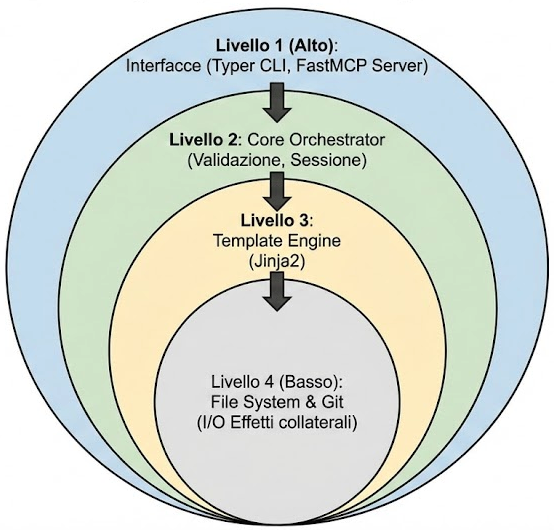
\includegraphics[width=0.6\textwidth]{images/strati_forge.png}
    \caption{Separazione delle responsabilità di service-forge [Elaborazione dell'autore].}
    \label{fig:onion_forge}
\end{figure}

A livello architetturale, il sistema concretizza la sua logica tramite pattern di progettazione consolidati. La Dependency Injection disaccoppia i componenti per agevolarne il testing unitario. Un pattern Factory istanzia dinamicamente i generatori appropriati in base al profilo di progetto selezionato (es. API sincrona, worker ETL). La separazione tra la generazione dei contenuti testuali e la loro persistenza su disco è mediata da un pattern Observer, mentre l'astrazione Strategy permette di mutare il comportamento di scaffolding in funzione del dominio applicativo.

\subsection{Sviluppo della Command Line Interface (CLI)}
L'interfaccia a riga di comando, sviluppata tramite la libreria Typer \cite{Typer}, guida l'operatore nella composizione interattiva della configurazione di progetto. Il flusso di esecuzione procede sequenzialmente: parte dalla selezione del profilo architetturale e dalla definizione del percorso fisico, per poi richiedere la configurazione dei servizi AWS necessari e dei parametri del runtime serverless. A valle dell'inserimento, il sistema esegue una validazione formale prima di delegare al motore centrale la generazione degli artefatti.

La CLI funge esclusivamente da livello di presentazione. Non contenendo logiche di scaffolding codificate rigidamente, essa raccoglie l'input e lo trasferisce al livello sottostante. Questa delega totale assicura una rigorosa coerenza comportamentale tra l'esecuzione manuale da terminale e l'esecuzione automatizzata tramite assistenti IA.

\subsection{Esposizione dei tool tramite Model Context Protocol (MCP)}
L'integrazione del framework con gli assistenti basati su Large Language Models operanti negli IDE avviene tramite un server conforme al Model Context Protocol, implementato avvalendosi della libreria FastMCP. Il server espone due categorie di astrazioni: risorse in sola lettura per la scoperta dei profili architetturali supportati, e strumenti operativi (Tools) necessari per la configurazione e la generazione del codice sorgente.

Durante la fase di inizializzazione, il server inietta nell'agente conversazionale un set di istruzioni testuali di sistema. Come illustrato nel Listato \ref{lst:mcp-init}, queste direttive vincolano il modello logico a richiedere esplicitamente all'operatore umano i parametri infrastrutturali reali (es. identificativi dei bucket S3 o nomi delle tabelle DynamoDB), prevenendo categoricamente la generazione di codice cloud contenente valori placeholder.

\begin{lstlisting}[language=Python, caption={Inizializzazione del server FastMCP con iniezione delle direttive operative e dei vincoli per l'agente LLM}, label={lst:mcp-init}]
from fastmcp import FastMCP

mcp = FastMCP(
    "service-forge",
    instructions=(
        "Service Forge generates AWS Lambda-based microservices. "
        "Use get_profiles to discover available profiles and services. "
        "IMPORTANT: Every AWS service has configurable parameters. "
        "Never use default placeholder values without asking the user first. "
        "Use create_session to start, then configure_service. "
        "Be sure to run check_prerequisites first."
    ),
)
\end{lstlisting}

\subsection{Interazione deterministica con i Large Language Models}
Il disaccoppiamento introdotto dall'MCP presenta una sfida architetturale: la comunicazione tra l'LLM e il server locale è intrinsecamente stateless. Per forzare un'interazione deterministica e limitare le allucinazioni del modello, il sistema delega il controllo del flusso al server locale tramite quattro vincoli architetturali: l'imposizione di una sequenza operativa rigorosa, la validazione strutturata dei payload di configurazione tramite Pydantic, l'obbligo di formattare le risposte in formato JSON standardizzato e l'integrazione di una funzionalità di simulazione (dry-run) per ispezionare l'astrazione generata senza alterare il file system.

Per supportare la sequenzialità delle operazioni, il server implementa un registro in memoria che associa a ogni sessione di interazione un identificativo alfanumerico univoco. Il Listato \ref{lst:mcp-session-state} dimostra come l'invocazione dello strumento \texttt{create\_session} istanzi una struttura dati predefinita contenente le dipendenze AWS e le configurazioni del runtime.

\begin{lstlisting}[language=Python, caption={Gestione del ciclo di vita e dello stato di sessione in memoria all'interno del server MCP}, label={lst:mcp-session-state}]
import uuid
from typing import Dict, Any

_sessions: Dict[str, Dict[str, Any]] = {}

@mcp.tool()
def create_session() -> str:
    session_id = str(uuid.uuid4())[:8]
    _sessions[session_id] = {
        "aws_services": {},
        "included_services": [],
        "runtime": dict(GenerationEngine.DEFAULT_RUNTIME),
    }
    return _json({"session_id": session_id})
\end{lstlisting}

Ogni successiva invocazione di uno strumento di configurazione o generazione richiede il passaggio obbligatorio di tale \texttt{session\_id} e modifica esclusivamente la porzione di stato isolata. Questo paradigma operativo riduce le ambiguità contestuali e assicura che il processo di generazione del microservizio rimanga prevedibile e tracciabile, indipendentemente dall'ambiente di sviluppo integrato (IDE) adottato dallo sviluppatore.

\chapter{Caso di Studio}
\label{chap:caso_studio}

La validazione empirica di un'architettura distribuita richiede un'analisi quantitativa volta a isolare le prestazioni dei singoli strati computazionali e di persistenza. Poiché i moderni paradigmi cloud-native disaccoppiano le fasi di ingestione, trasformazione e presentazione delle informazioni, una valutazione olistica risulterebbe imprecisa. Per tale motivo logico, il presente capitolo frammenta l'indagine in tre fasi distinte, progettate per misurare progressivamente l'impatto delle singole scelte implementative. La prima fase definisce la metodologia di collaudo. La seconda fase analizza le prestazioni dei processi asincroni di elaborazione dati. Infine, la terza fase quantifica le latenze dei servizi sincroni e i tempi di approvvigionamento infrastrutturale.

L'ambiente di collaudo consiste in un'infrastruttura di laboratorio progettata per fungere da setting simulato di un ecosistema aziendale operante nel dominio dell'advertising digitale. Per garantire la validità scientifica delle misurazioni senza fare affidamento su generatori di traffico sintetico, l'ambiente isolato si interfaccia direttamente con le piattaforme esterne di produzione. Il sistema elabora parametri e volumi di traffico estratti da un reale caso industriale aziendale, il quale ha fornito le autorizzazioni necessarie per l'interrogazione dei dati.

Questo approccio metodologico garantisce che i volumi di carico, quantificati in circa trenta Gigabyte mensili di dati grezzi, e le latenze di rete registrate riflettano fedelmente la complessità operativa di uno scenario autentico. L'infrastruttura di monitoraggio delega la raccolta dei dati ai componenti nativi del provider cloud, come Amazon CloudWatch e Amazon Athena, generando metriche oggettive sul comportamento del sistema sotto sforzo.

\section{Obiettivi della Valutazione}
L'implementazione dell'architettura software fornisce i componenti tecnici per l'elaborazione dei flussi informativi ad alto volume. Tuttavia, la sola definizione dell'infrastruttura tramite il paradigma Infrastructure as Code governato da Terraform non è sufficiente a dimostrare il superamento dei limiti operativi riscontrati nei sistemi tradizionali. Un'architettura distribuita necessita di una validazione quantitativa per confermare la scalabilità e la stabilità delle prestazioni sotto carico.

\section{Metodologia di Collaudo e Strumenti di Telemetria}
Il collaudo dell'architettura prescinde dall'iniezione di traffico artificiale, adottando una metodologia di analisi osservazionale basata sui carichi di lavoro organici estratti da sistemi in produzione. La validazione empirica aggrega e analizza statisticamente i dati di telemetria raccolti in un arco temporale definito, valutando il comportamento del sistema a regime. L'esclusione di strumenti di stress testing attivi garantisce che le misurazioni riflettano le latenze di rete effettive e i pattern di accesso tipici delle integrazioni tra sistemi distribuiti.

La piattaforma cloud delega la raccolta dei dati a due servizi nativi. Il primo strumento è Amazon CloudWatch, impiegato per il campionamento delle metriche prestazionali a livello di infrastruttura. L'analisi estrae tramite questo servizio i tempi di esecuzione delle funzioni AWS Lambda (metrica \texttt{Duration}), l'allocazione della memoria e il consumo di capacità di lettura e scrittura delle tabelle Amazon DynamoDB. Il servizio provvede inoltre al calcolo automatico dei percentili statistici ($p50$, $p90$, $p99$) relativi alle latenze di integrazione esposte da Amazon API Gateway.

Il secondo strumento di validazione quantitativa risiede nelle metriche di esecuzione di Amazon Athena. Il motore di query traccia il volume di dati scansionati e i millisecondi di elaborazione per ciascuna transazione SQL. L'incrocio di questi valori con la topologia del partizionamento fisico su Amazon S3 fornisce le evidenze necessarie per dimostrare il contenimento della complessità computazionale e il conseguente abbattimento dei costi operativi.

\section{Caso di Studio I: Pipeline ETL Asincrona}
Il primo caso di studio esamina la pipeline ETL incaricata di ingerire la reportistica generata da piattaforme esterne di ad-serving \cite{GoogleAdManager}. L'elaborazione di tali flussi informativi estrae metriche granulari sulle campagne pubblicitarie, fornendo dati aggregati su impressioni, costi e formati. L'architettura applica i pattern definiti nei capitoli precedenti per eseguire l'estrazione periodica di questi dataset complessi. L'obiettivo dell'analisi consiste nel validare la stabilità del runtime Serverless in elaborazioni prolungate e misurare l'efficienza della compressione dei dati.

\subsection{Scenario Operativo e Prestazioni di Estrazione}
Lo scenario operativo impiega regole temporali su Amazon EventBridge, le quali governano l'esecuzione del livello di estrazione isolando le singole transazioni. Come illustrato nella Figura \ref{fig:cloudwatch-extractor}, l'aggregazione delle metriche rileva un regime stabile di circa 140-150 invocazioni giornaliere. Il sistema dimostra la capacità di scalare orizzontalmente, assorbendo picchi di oltre 3.200 invocazioni giornaliere senza registrare degrado prestazionale durante le fasi di ri-computazione dei dati storici.

\begin{figure}[htbp]
\centering
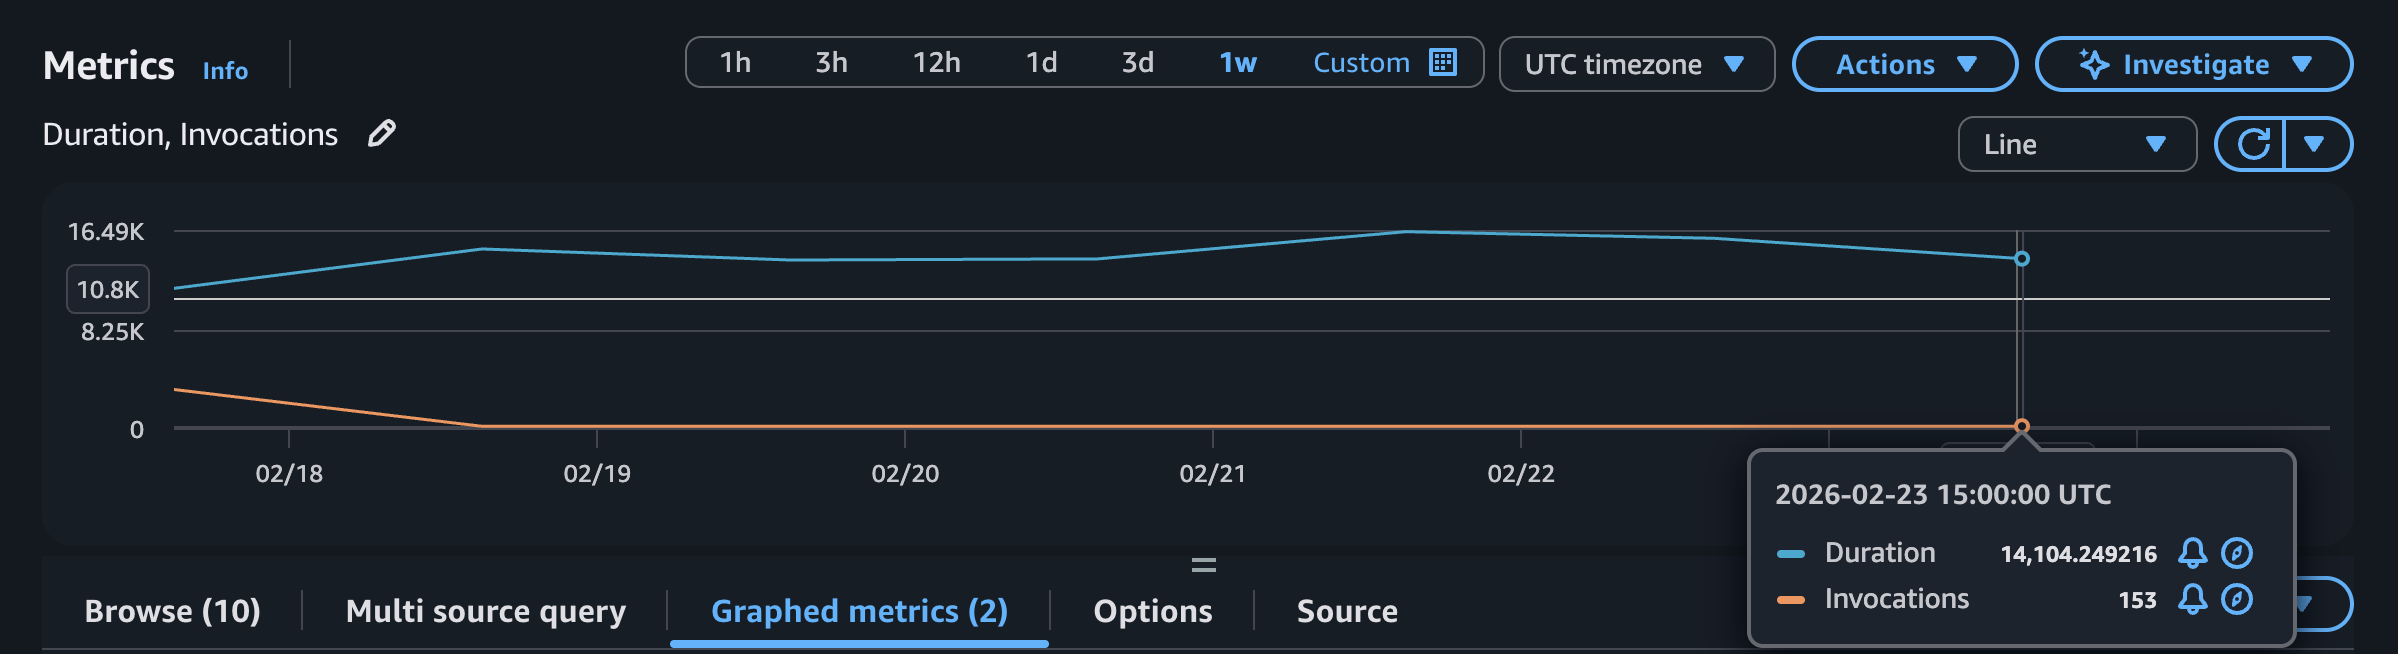
\includegraphics[width=1\textwidth]{images/invocations-durations-extractor.png}
\caption{Grafico CloudWatch illustrante il volume di invocazioni e la metrica Duration del livello Extractor.}
\label{fig:cloudwatch-extractor}
\end{figure}

L'analisi della metrica di durata evidenzia un tempo medio di esecuzione per l'estrazione dati compreso tra $14.000$ e $16.350$ millisecondi per singola invocazione. Questo valore certifica che il componente opera con un margine di tolleranza elevato rispetto al vincolo massimo di 900 secondi imposto dal provider. Il tasso di errore di rete, registrato allo $1,3\%$, giustifica empiricamente l'implementazione della logica di ritentativo applicativo e l'uso delle Dead Letter Queue (DLQ).

\subsection{Efficienza della Trasformazione in Memoria}
La fase di trasformazione, responsabile dell'appiattimento e della sanificazione dei documenti JSON, sfrutta la libreria Polars per l'elaborazione vettoriale in memoria. Le metriche documentano un tempo medio di esecuzione pari a $1.160$ millisecondi, con un tasso di errore dello $0\%$, come indicato nella Figura \ref{fig:transformer-graphic}. Tale efficienza computazionale previene la saturazione della memoria preallocata all'interno dei container.

\begin{figure}[htbp]
\centering
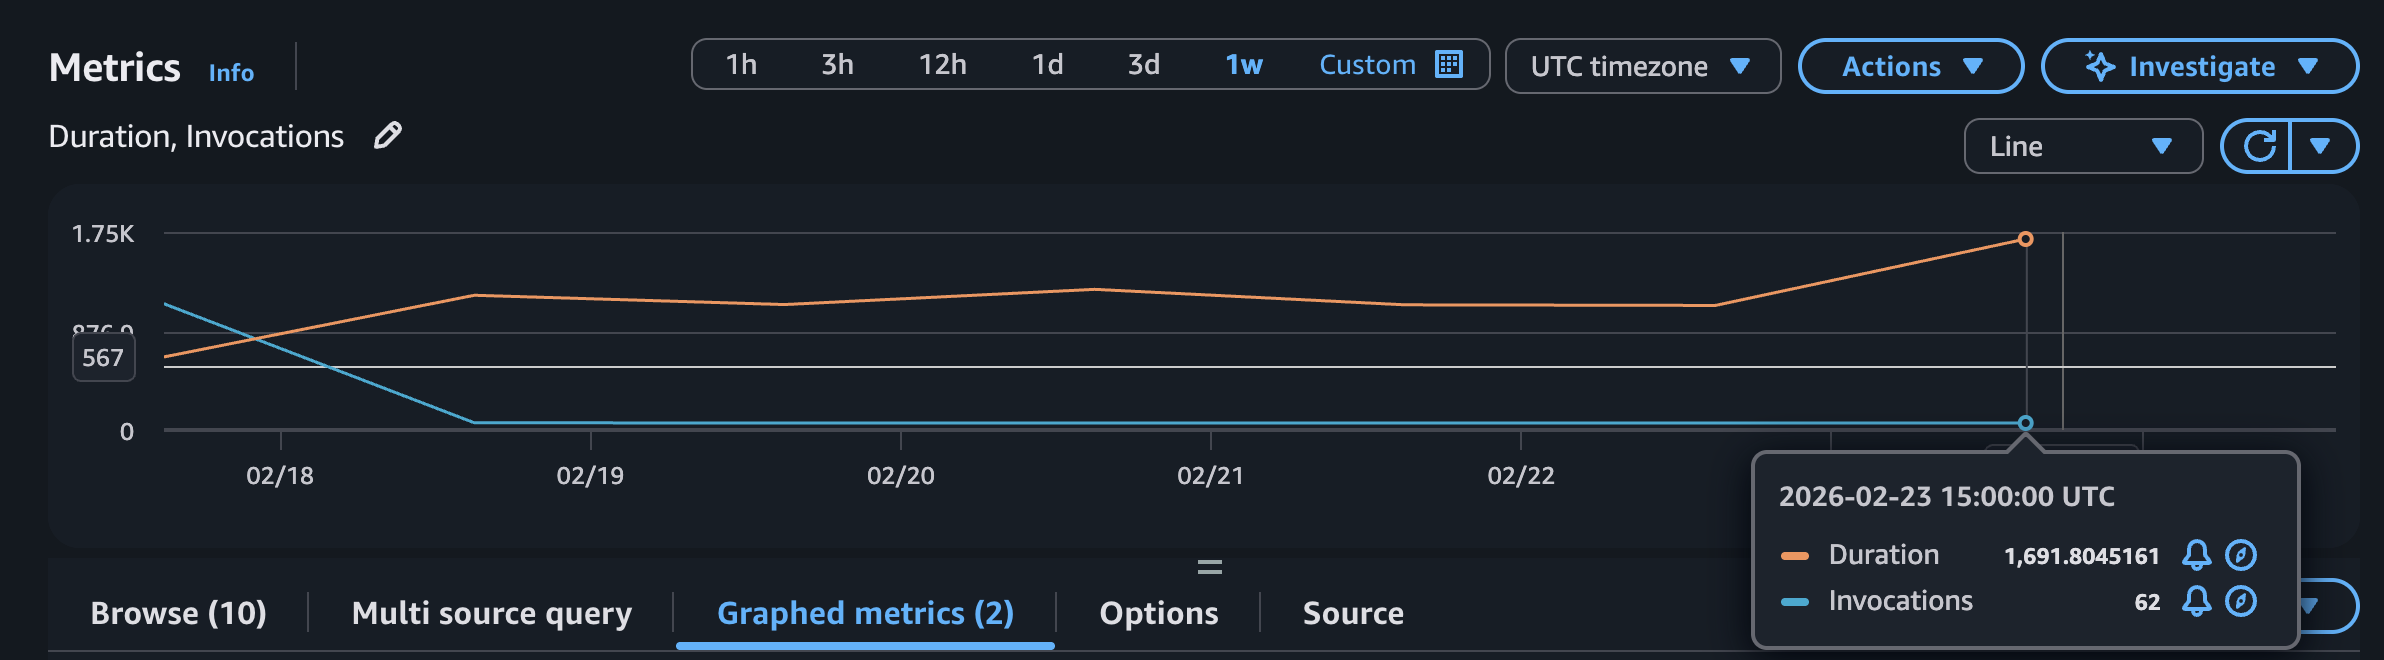
\includegraphics[width=1\textwidth]{images/invocations-durations-transformer.png}
\caption{Grafico CloudWatch illustrante il volume di invocazioni e la metrica Duration del livello Transformer.}
\label{fig:transformer-graphic}
\end{figure}

Come riportato nella Tabella \ref{tab:dimensionale-parquet}, la serializzazione finale in formato Apache Parquet con algoritmo di compressione Snappy produce una riduzione misurabile del footprint di archiviazione.

\begin{table}[htbp]
\centering
\caption{Confronto dimensionale empirico tra i payload estratti (Raw JSON/CSV) e i file ottimizzati (Clean Parquet).}
\label{tab:dimensionale-parquet}
\small
\begin{tabularx}{\textwidth}{lRR}
\toprule
\textbf{Tipologia di Report} & \textbf{Dimensione Raw} & \textbf{Dimensione Clean (Parquet)} \\
\midrule
get\_all\_line\_items & 654.6 MB & 1.6 MB \\
open\_header\_bidding & 161.2 MB & 45.7 MB \\
key\_value & 24.4 MB & 40.9 MB \\
kpis\_by\_hour & 3.7 MB & 2.0 MB \\
adrequest\_by\_hour & 1.4 MB & 921.3 KB \\
get\_all\_custom\_fields & 27.1 KB & 6.0 KB \\
\bottomrule
\end{tabularx}
\end{table}

Il fattore di compressione incide in misura maggiore sui documenti di grandi dimensioni, riducendo il file \texttt{get\_all\_line\_items} di un fattore superiore a 400. Eventuali incrementi dimensionali su file nell'ordine dei byte costituiscono un comportamento fisiologico imputabile alla dimensione minima dei metadati intrinseci richiesti dallo schema Parquet.

\subsection{Ottimizzazione dell'Interrogazione tramite Partition Pruning}
L'ultima fase del collaudo per la pipeline asincrona valuta l'impatto del partizionamento logico sui costi operativi e sulle latenze di Amazon Athena. L'indagine quantifica l'efficienza algoritmica della topologia a partizioni multiple, organizzata gerarchicamente per anno, mese e giorno. Il test esegue una serie di interrogazioni SQL sulla tabella non aggregata relativa alle impressioni pubblicitarie. La Tabella \ref{tab:athena-performance} sintetizza i risultati prestazionali estratti dal servizio cloud.

\begin{table}[htbp]
\centering
\caption{Confronto analitico delle prestazioni di scansione del motore distribuito Amazon Athena.}
\label{tab:athena-performance}
\small
\begin{tabularx}{\textwidth}{Xrr}
\toprule
\textbf{Modalità di Interrogazione} & \textbf{Tempo di Esecuzione} & \textbf{Dati Scansionati} \\
\midrule
Scansione Completa (Assenza di partizioni) & 15,37 secondi & 3,82 GB \\
Scansione Ottimizzata (Partition Pruning applicato) & 541 millisecondi & 3,90 MB \\
\bottomrule
\end{tabularx}
\end{table}

Il primo scenario di test definisce l'esecuzione di una query aggregata sull'intero storico dei dati. L'assenza di predicati temporali forza il motore distribuito a eseguire una scansione sequenziale completa dei file archiviati. Come illustrato nella Figura \ref{fig:athena-full-scan}, l'operazione comporta la lettura di $3,82$ GB di dati in $15,3$ secondi, impegnando le risorse in modo direttamente proporzionale alla dimensione totale del Data Lake.

\begin{figure}[htbp]
\centering
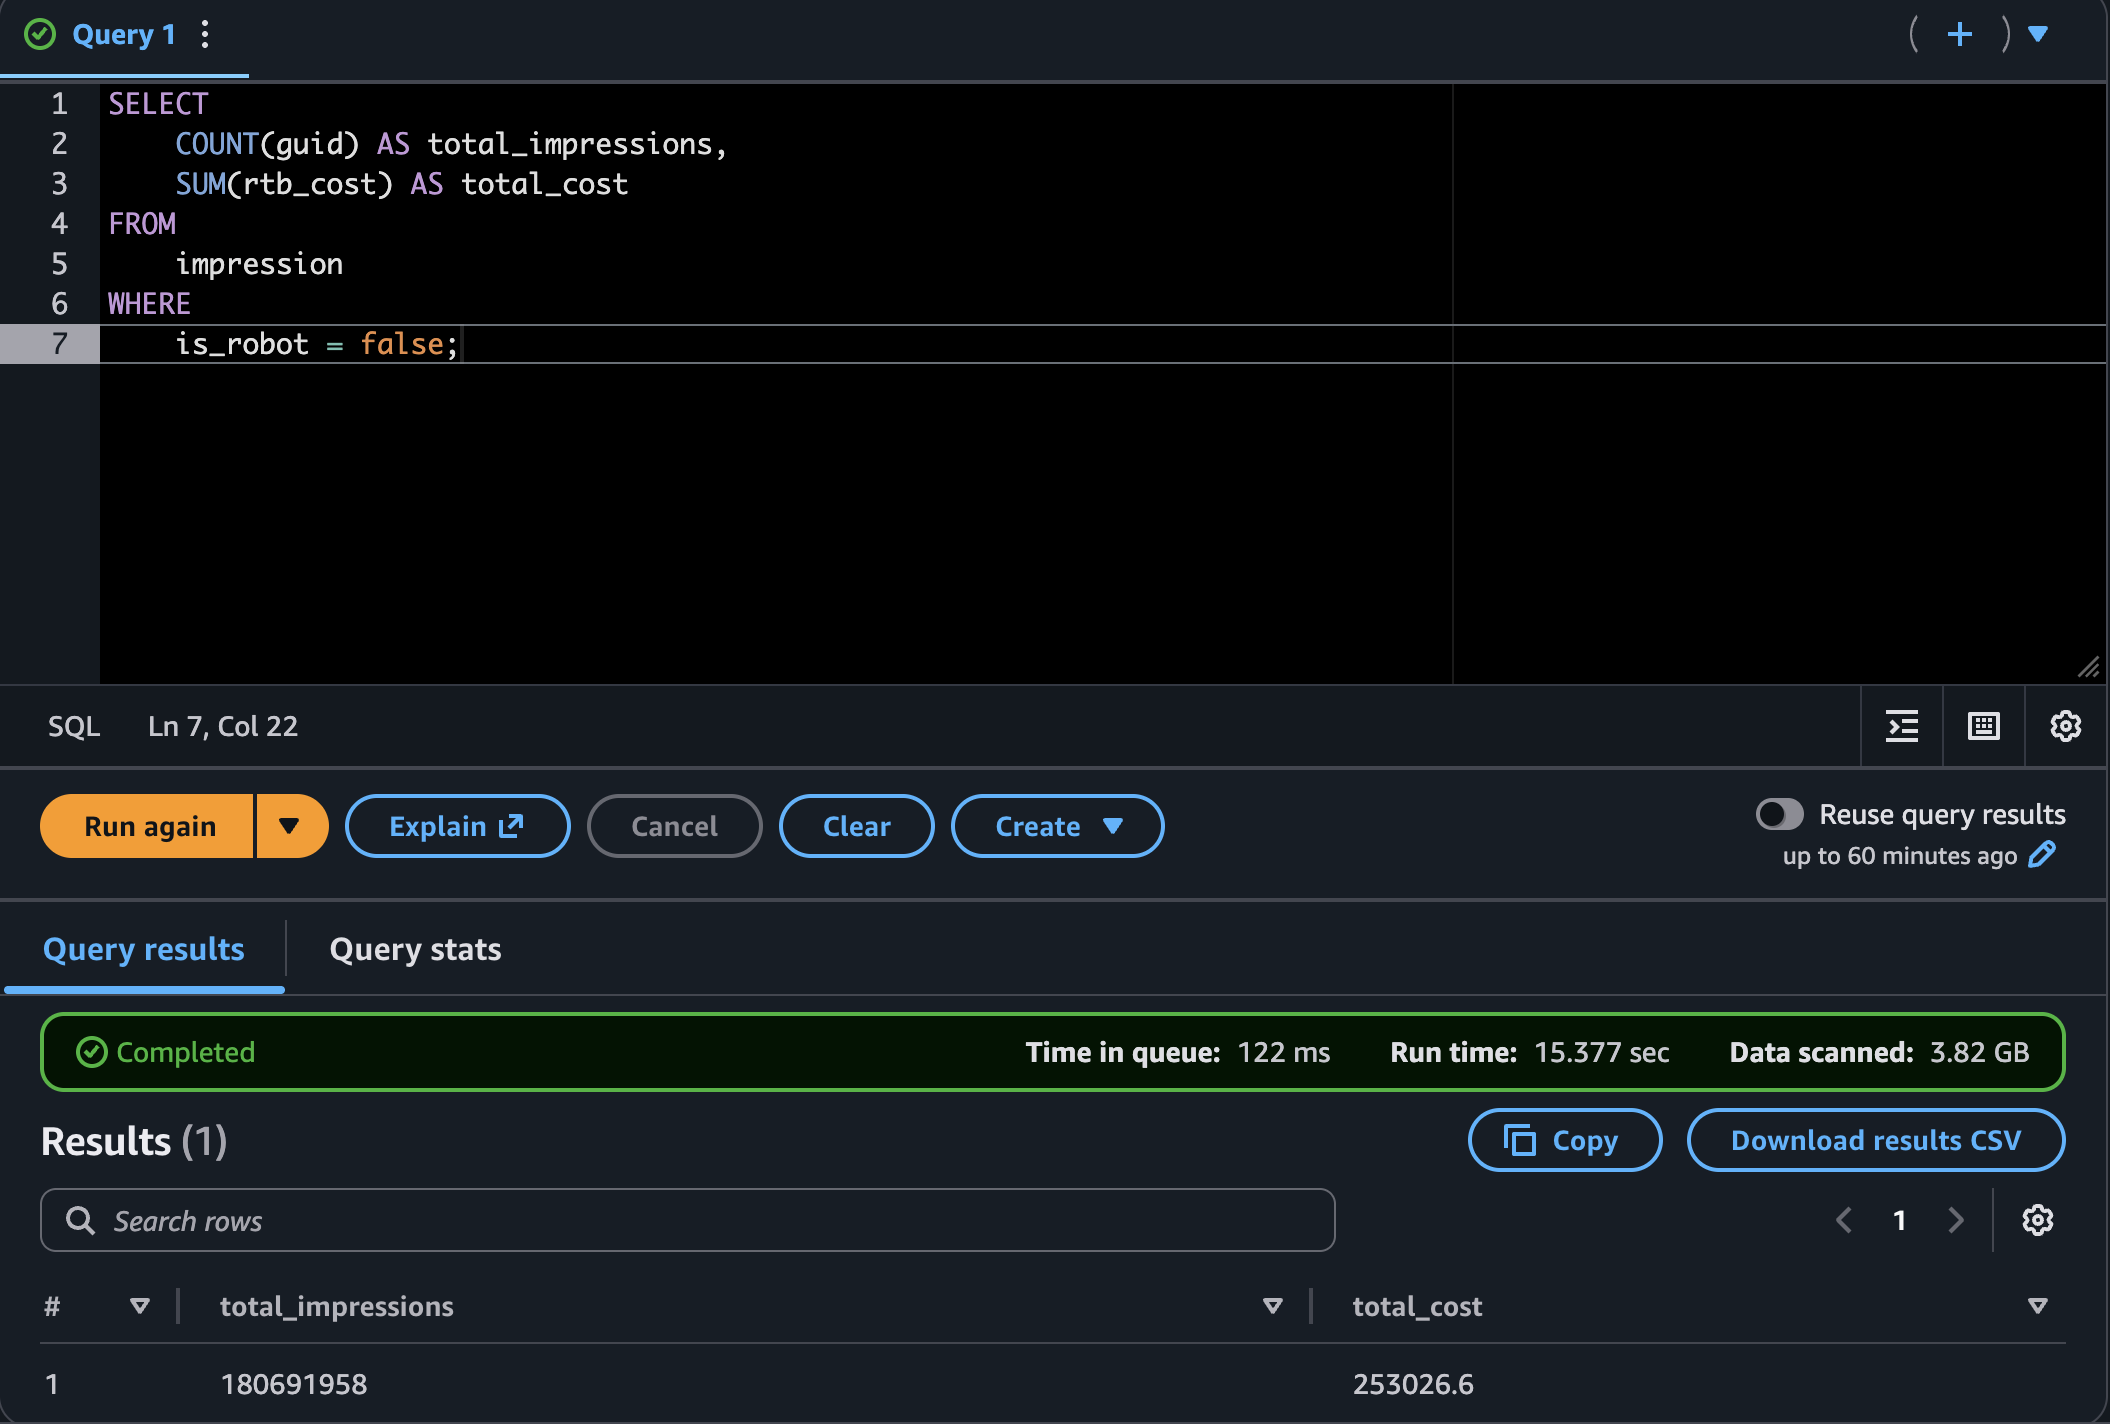
\includegraphics[width=\textwidth]{images/athena_full_scan.png}
\caption{Interfaccia di Amazon Athena: esecuzione di una query priva di partizionamento.}
\label{fig:athena-full-scan}
\end{figure}

Il secondo scenario applica il meccanismo di partition pruning, introducendo predicati temporali nella clausola \texttt{WHERE} per restringere il perimetro di ricerca a una singola giornata operativa. Il motore di Athena interroga il catalogo dati per escludere i prefissi non pertinenti prima di accedere allo storage. La Figura \ref{fig:athena-partition-pruning} riporta i risultati prestazionali di questa seconda esecuzione.

\begin{figure}[htbp]
\centering
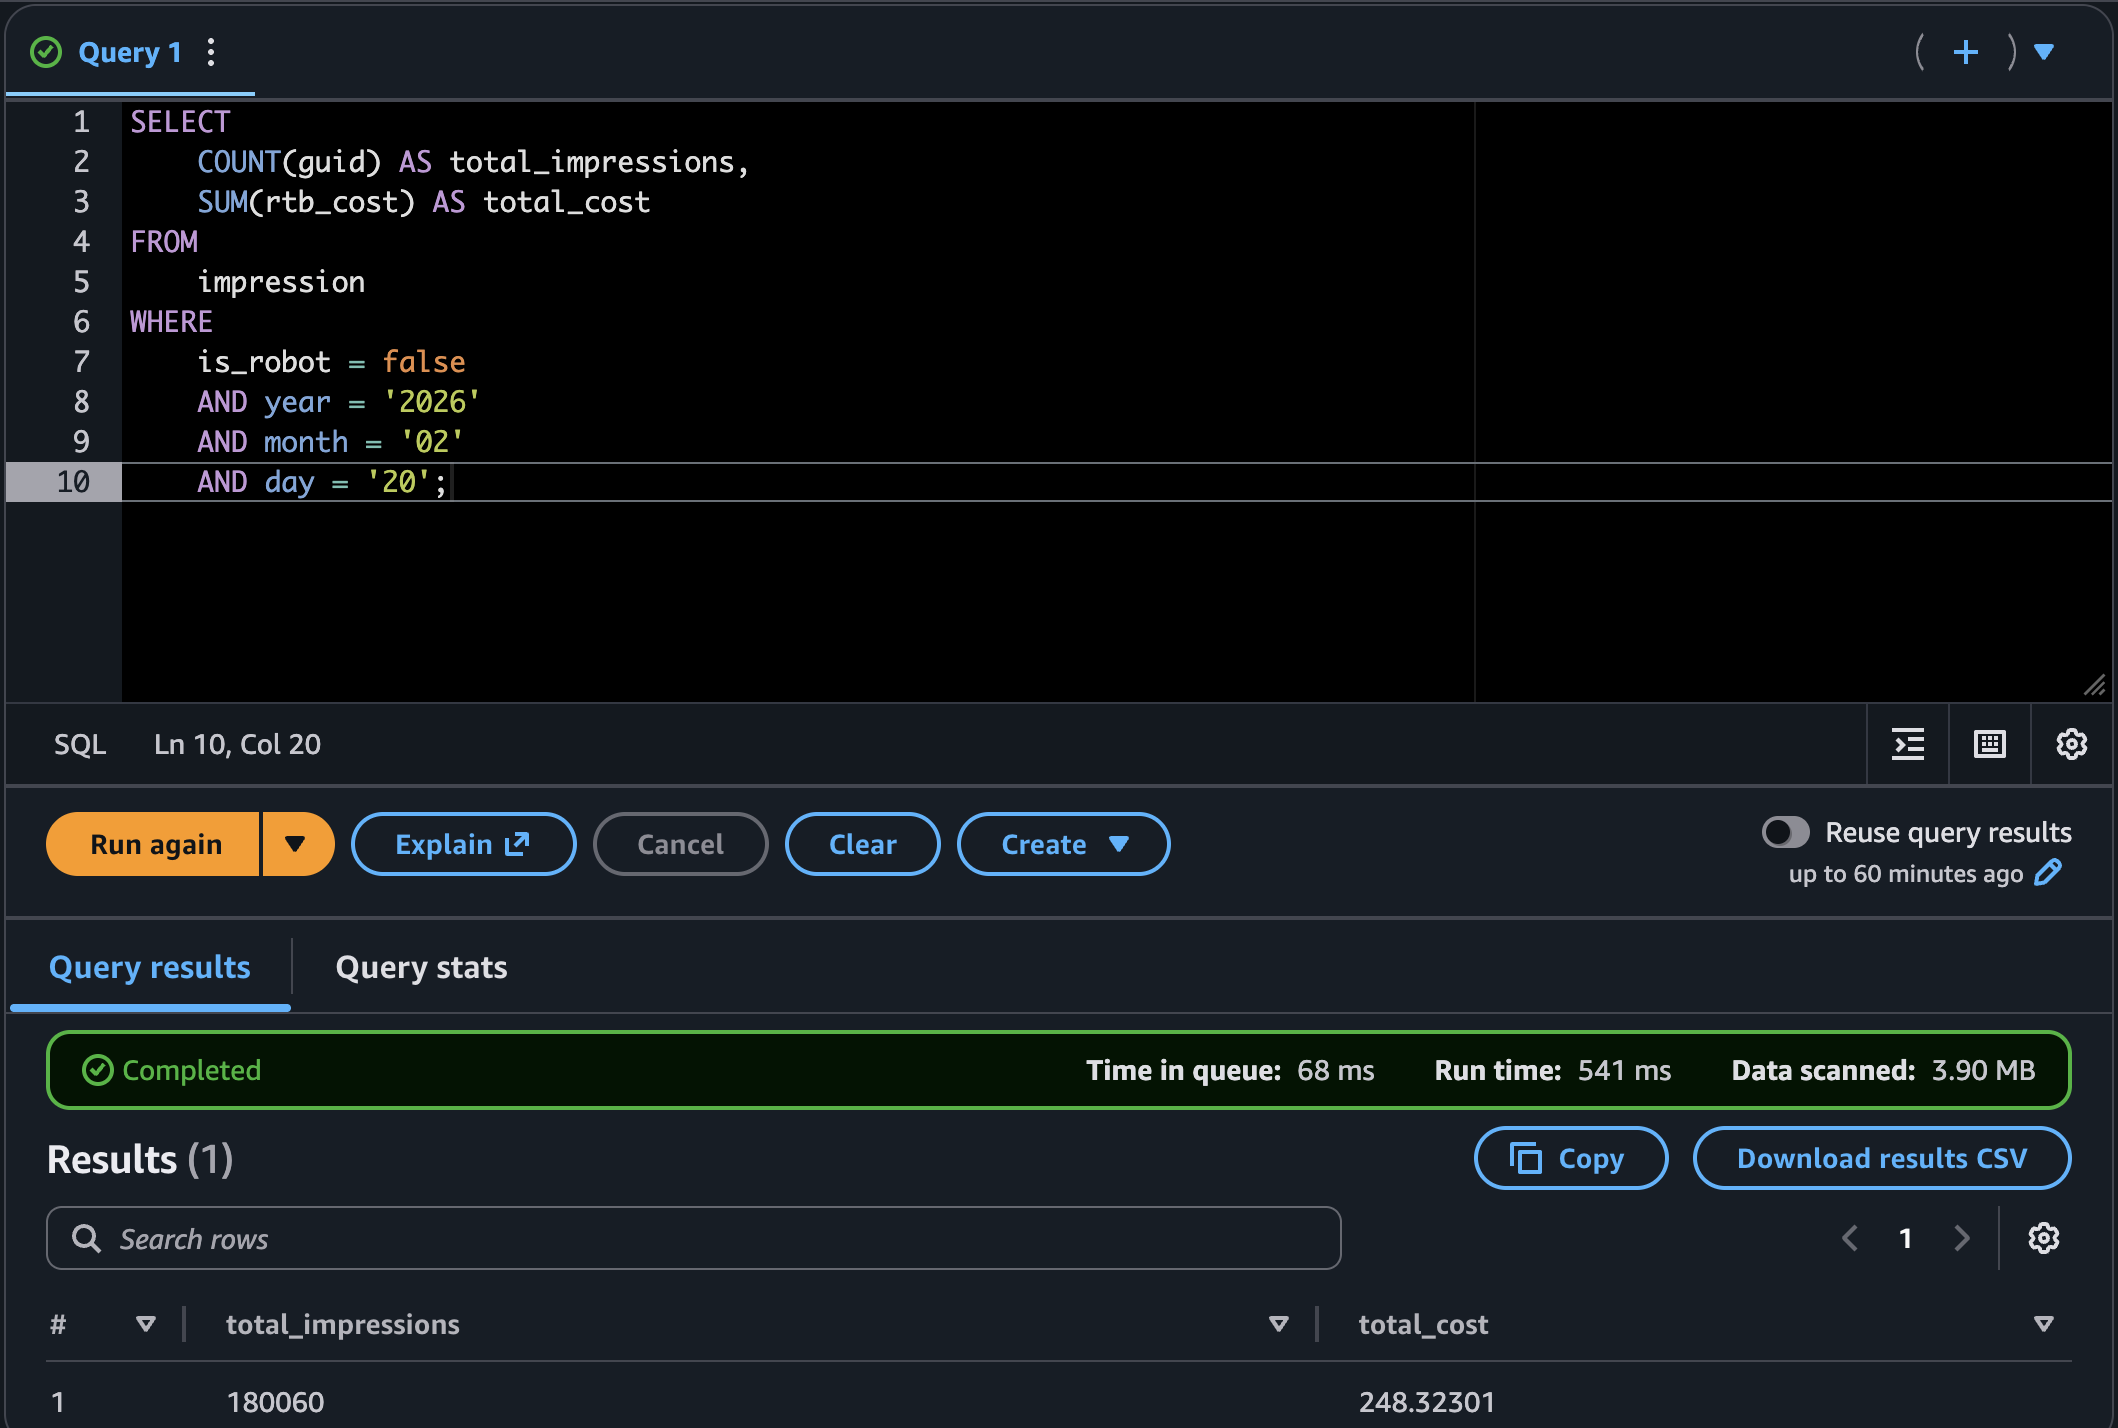
\includegraphics[width=\textwidth]{images/athena_optimized_scan.png}
\caption{Interfaccia di Amazon Athena: esecuzione di una query ottimizzata tramite partition pruning.}
\label{fig:athena-partition-pruning}
\end{figure}

Il partizionamento logico riduce il volume dei dati scansionati a $3,90$ MB e abbatte il tempo di elaborazione a $541$ millisecondi. L'abbattimento delle letture su disco dimostra che l'isolamento deterministico dei prefissi disaccoppia il tempo e il costo di interrogazione dalla mole totale dei dati immagazzinati nel sistema.

\section{Analisi quantitativa dei costi}
L'indagine economica valuta l'impatto del paradigma Serverless confrontando il modello a consumo con l'allocazione statica delle risorse, impiegando i parametri di fatturazione per la regione eu-west-1. L'analisi utilizza i dati volumetrici misurati nel primo caso di studio durante una settimana operativa. La quantificazione economica si struttura su due vettori di costo: il livello di archiviazione per le interrogazioni interattive e il livello computazionale per la trasformazione dei dati.

Il primo parametro esaminato riguarda il livello di interrogazione tramite Amazon Athena, il cui modello prevede un costo fisso di $\$5.00$ per terabyte scansionato. La sorgente dati genera 994 Megabyte di dati grezzi giornalieri, equivalenti a circa 30 Gigabyte mensili. In assenza di ottimizzazioni, una singola query sulla giornata imporrebbe la lettura dell'intero archivio, generando un addebito di $\$0.14$. Il processo ETL converte i file in formato Parquet riducendo l'impronta a 107 Megabyte giornalieri, e il partizionamento logico istruisce il motore a leggere unicamente questa frazione. La convergenza di queste tecniche porta il costo della singola operazione a $\$0.0005$, confermando la sostenibilità finanziaria del sistema analitico.

Il secondo parametro economico concerne l'elaborazione computazionale. La funzione AWS Lambda di estrazione esegue 4079 invocazioni settimanali (50244 secondi di calcolo), mentre la trasformazione registra 1498 invocazioni (1215 secondi). Entrambe richiedono 6 Gigabyte di memoria. Proiettando le metriche su base mensile, l'infrastruttura consuma circa $1.32$ milioni di Gigabyte-secondo, traducendosi in una spesa di $\$17.65$ mensili sull'architettura ARM. Un'architettura tradizionale basata su un'istanza Amazon EC2 \cite{EC2} di classe c6g.xlarge (4 vCPU, 8 GB RAM) imporrebbe un costo fisso di $\$103.95$. Il modello basato su eventi riduce i costi di elaborazione dell'$83\%$, eliminando il dispendio economico intrinseco ai periodi di inattività.

\section{Caso di Studio II: Servizio Backend Sincrono}
Il secondo caso di studio valuta l'architettura a fronte di carichi operativi sincroni. Il perimetro di analisi coinvolge un'API interna sviluppata tramite il framework FastAPI ed esposta via API Gateway, concepita per la registrazione e il recupero dei metadati relativi a presentazioni multimediali. L'implementazione applica i paradigmi di astrazione precedentemente descritti per misurare le latenze di un'infrastruttura di backend interamente gestita dal cloud provider.

\subsection{Modello Dati ad Alta Efficienza}
La memorizzazione dello stato sfrutta il database NoSQL Amazon DynamoDB. La progettazione adotta il paradigma Single Table Design, modellato tramite la libreria PynamoDB. L'entità definisce una chiave di partizione primaria per l'accesso puntuale a complessità costante. Per supportare le interrogazioni sulle collezioni, la struttura implementa un Global Secondary Index (GSI) con chiave di partizione statica e chiave di ordinamento cronologica, come mostrato nel Listato \ref{lst:demoland-pynamo}.

\begin{lstlisting}[language=Python, caption={Modellazione Object-Relational Mapping (ORM) su DynamoDB.}, label={lst:demoland-pynamo}]
from pynamodb.models import Model
from pynamodb.attributes import UnicodeAttribute, BooleanAttribute
from pynamodb.indexes import GlobalSecondaryIndex, AllProjection
import os

class CreationDateIndex(GlobalSecondaryIndex):
    """
    This class represents a GSI for querying previews by creation_date.
    """
    class Meta:
        index_name = 'creation-date-index'
        projection = AllProjection()
    
    # This attribute will be the partition key for the GSI
    entity_type = UnicodeAttribute(hash_key=True)
    creation_date = UnicodeAttribute(range_key=True)

class Preview(Model):
    class Meta:
        table_name = os.environ.get("DYNAMODB_TABLE")
        region = os.getenv("AWS_DEFAULT_REGION")
    
    # GSI for sorting by creation_date
    creation_date_index = CreationDateIndex()

    # Primary key
    slug = UnicodeAttribute(hash_key=True)
    SLUG_MAX_ATTEMPTS = 10

    # GSI partition key - a static value to query all previews
    entity_type = UnicodeAttribute(default="PREVIEW")

    # Client and campaign information
    customer = UnicodeAttribute()
    normalized_customer = UnicodeAttribute()
    campaign = UnicodeAttribute()
    normalized_campaign = UnicodeAttribute()

    # Categorization fields
    vertical = UnicodeAttribute()
    format = UnicodeAttribute()
    type = UnicodeAttribute()

    # Technical fields
    webpage = UnicodeAttribute()
    script = UnicodeAttribute()

    # Configuration flags
    confidential = BooleanAttribute(default=False)
    live = BooleanAttribute(default=False)
    device = UnicodeAttribute(default="Mobile")

    # Location and language
    delivery_country = UnicodeAttribute(default="Italy")
    language = UnicodeAttribute(default="Italian")
    country = UnicodeAttribute(default="Simulated Entity")

    # Creation date
    creation_date = UnicodeAttribute(null=True)
\end{lstlisting}

Come evidenziato nella Tabella \ref{tab:dynamodb-capacity} e nella Figura \ref{fig:dynamodb-capacity}, la standardizzazione degli accessi limita il consumo delle unità di capacità di lettura e scrittura.

\begin{table}[htbp]
\centering
\caption{Medie di consumo orario delle unità di capacità sul livello DynamoDB.}
\label{tab:dynamodb-capacity}
\begin{tabular}{lr}
\toprule
\textbf{Metrica di Capacità (Media Oraria)} & \textbf{Valore Rilevato} \\
\midrule
Consumed Read Capacity Units (RCU) & 0.005 \\
Consumed Write Capacity Units (WCU) & 0.062 \\
\bottomrule
\end{tabular}
\end{table}

\begin{figure}[htbp]
\centering
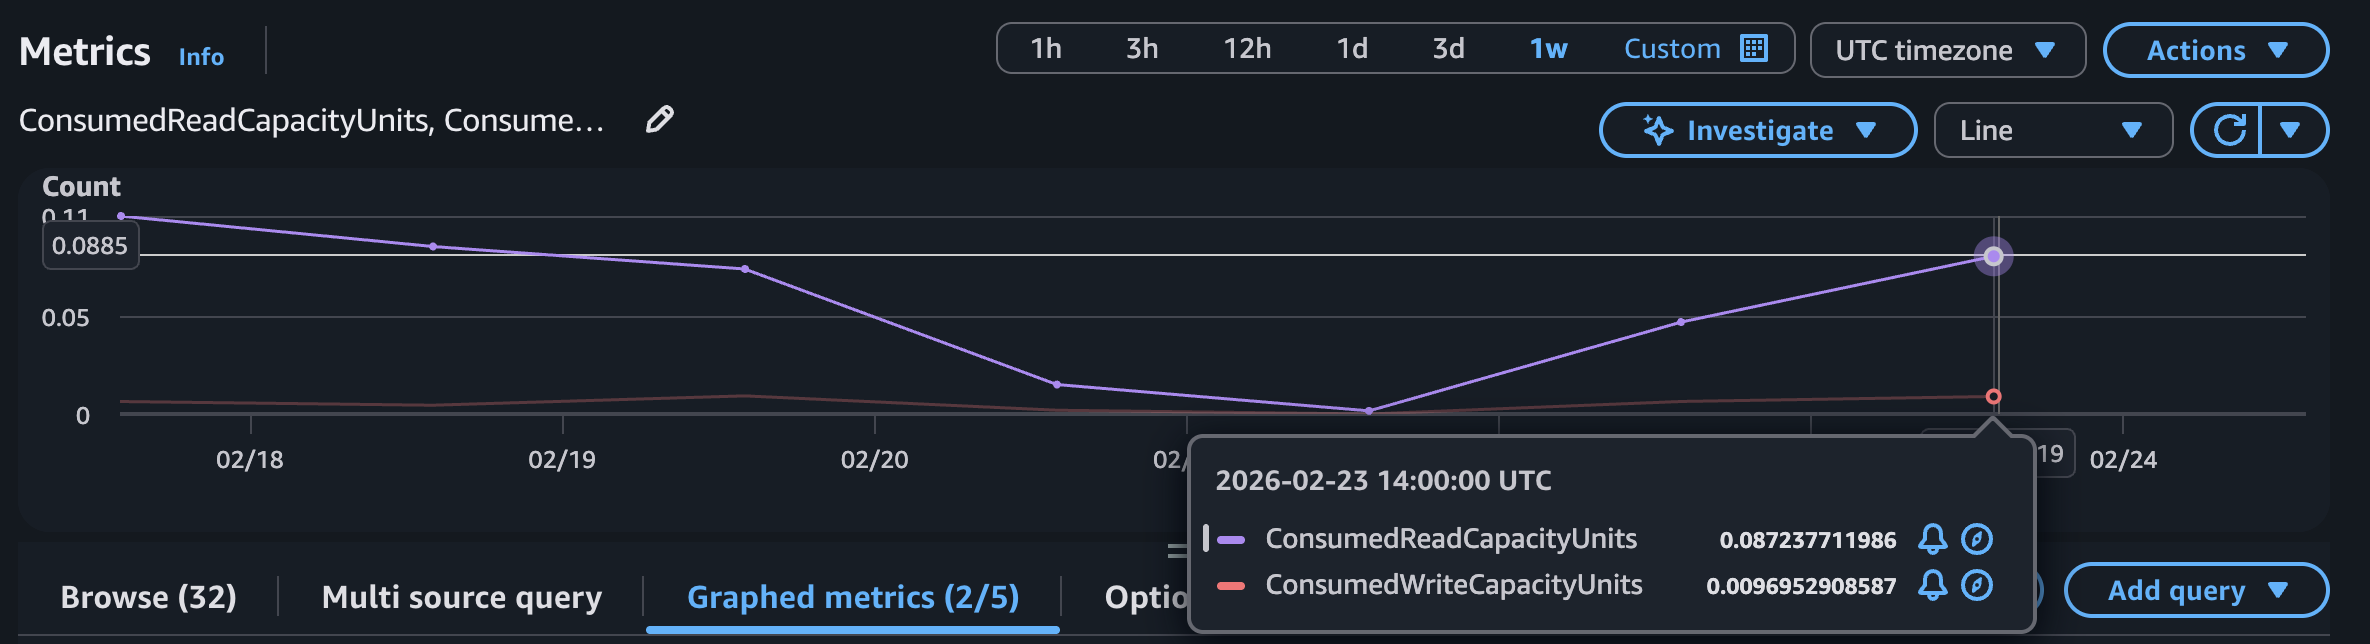
\includegraphics[width=1\textwidth]{images/capacity-dynamo.png}
\caption{Grafico CloudWatch illustrante l'andamento temporale della capacity di DynamoDB per il servizio.}
\label{fig:dynamodb-capacity}
\end{figure}

Il contenimento delle capacità consumate garantisce la scalabilità del catalogo limitando l'impatto economico associato alle operazioni concorrenti.

\subsection{Distribuzione Statistica della Latenza e Cold Start}
L'esecuzione del framework web all'interno dell'ambiente di calcolo effimero necessita dell'adattatore Mangum. La telemetria calcola i percentili statistici dei tempi di integrazione esposti all'utente per misurare l'incidenza di questo strato di traduzione. I dati aggregati sono presentati nella Tabella \ref{tab:percentili-latenza} e graficati nella Figura \ref{fig:api-gateway-latency}.

\begin{table}[htbp]
\centering
\caption{Distribuzione statistica dei percentili di latenza di integrazione (in millisecondi).}
\label{tab:percentili-latenza}
\begin{tabular}{lr}
\toprule
\textbf{Percentile Statistico} & \textbf{Latenza Rilevata (ms)} \\
\midrule
50° Percentile ($p50$ - Mediana) & 19.5 ms \\
90° Percentile ($p90$) & 708.5 ms \\
99° Percentile ($p99$) & 1751.9 ms \\
\bottomrule
\end{tabular}
\end{table}

\begin{figure}[htbp]
\centering
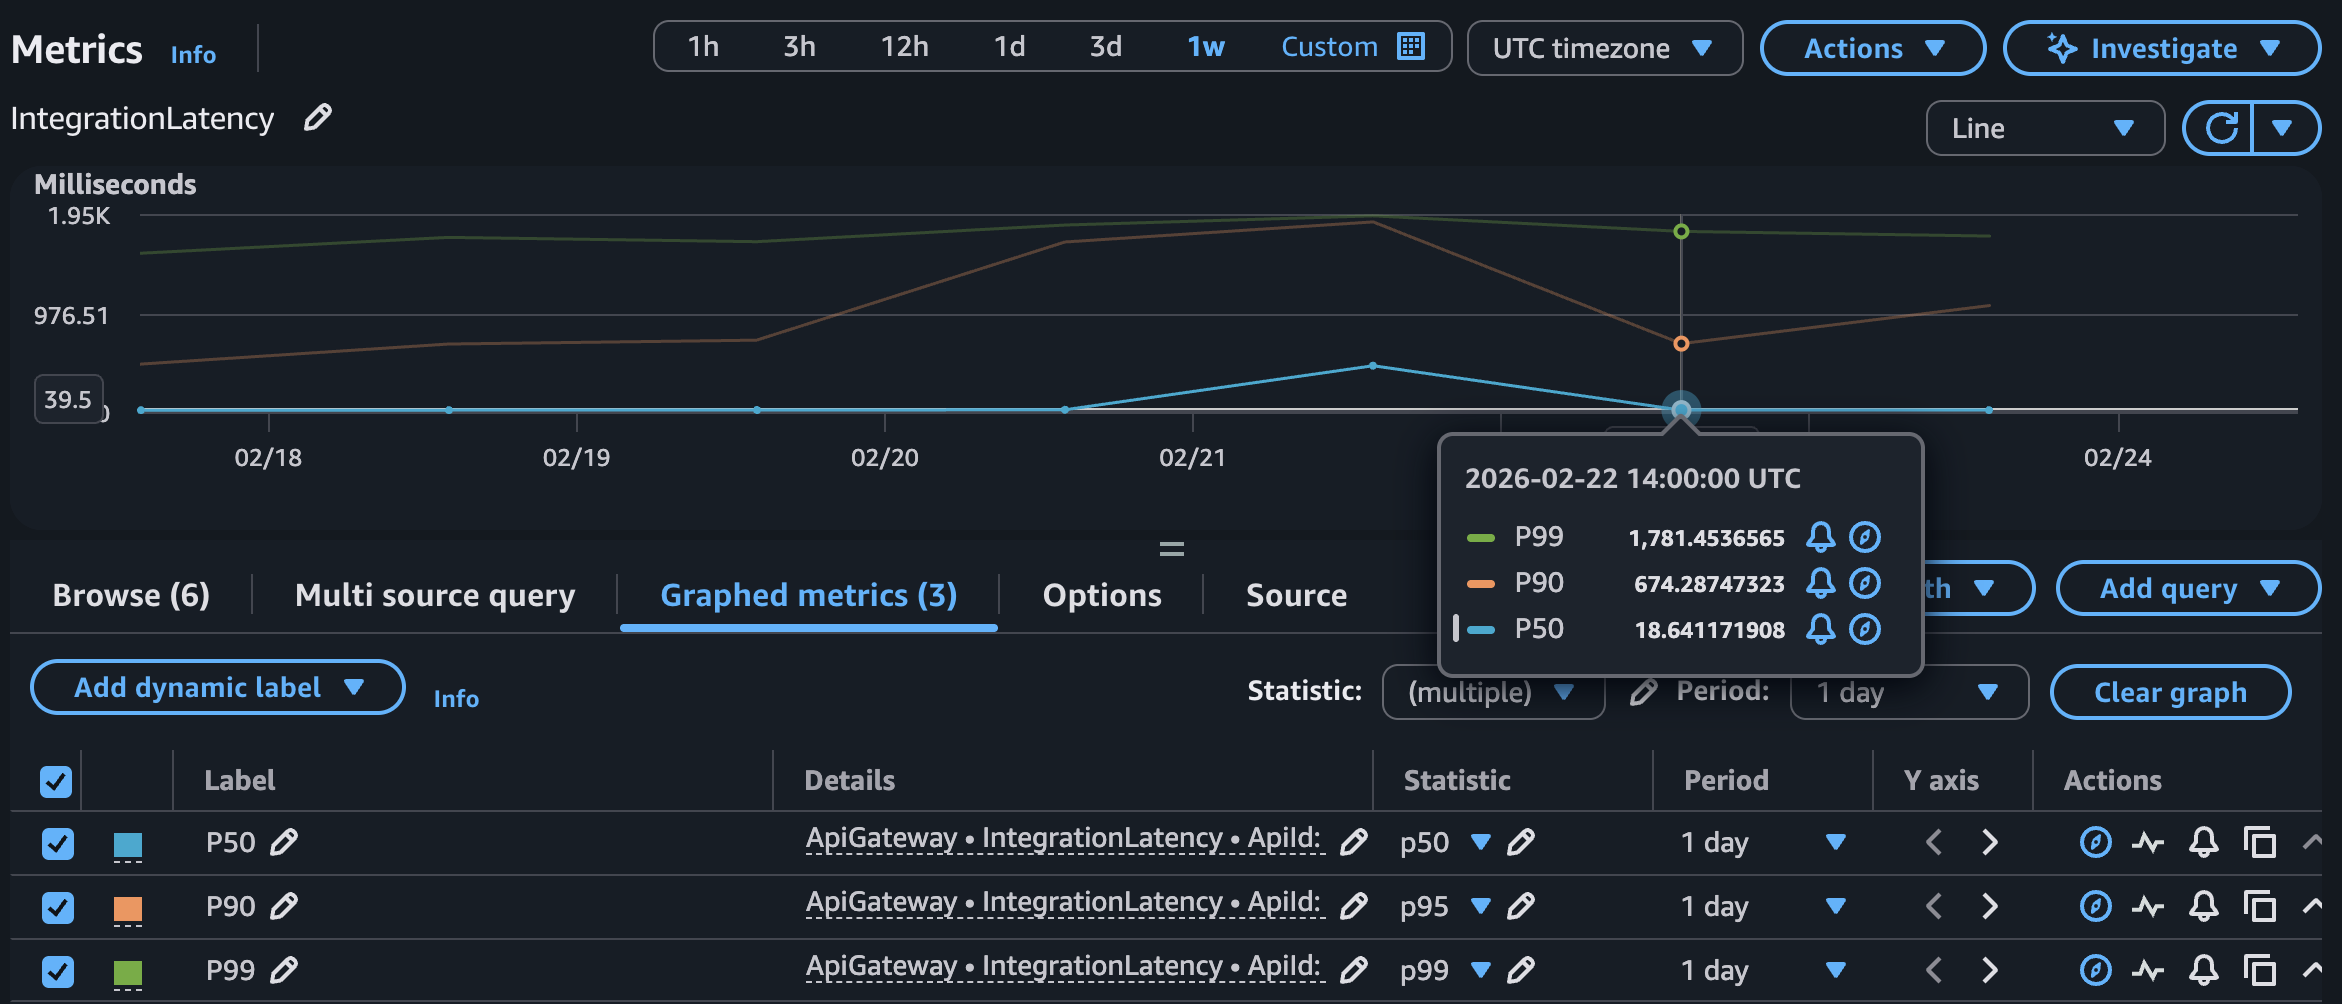
\includegraphics[width=1\textwidth]{images/percentili-api-gateway.png}
\caption{Grafico CloudWatch illustrante l'andamento temporale dei percentili di latenza p50, p90 e p99.}
\label{fig:api-gateway-latency}
\end{figure}

Il tempo di risposta mediano ($p50$) attesta che l'adattatore non introduce sovraccarichi penalizzanti nei container già in esecuzione. L'analisi dei percentili di coda ($p90$ e $p99$) quantifica empiricamente il peso delle latenze di inizializzazione dell'ambiente (Cold Start), le quali portano i tempi di risposta oltre la soglia dei 1700 millisecondi. La varianza rientra nei limiti di tolleranza per i requisiti non funzionali del sistema in analisi.

\section{Valutazione dell'Automazione Infrastrutturale (Service-Forge)}
L'ultima fase dell'analisi quantifica l'impatto architetturale derivante dall'adozione del framework interno dedicato allo scaffolding. Il sistema standardizza il provisioning di nuovi microservizi astraendo la complessità dichiarativa dell'Infrastructure as Code (IaC). La valutazione esamina tre distinte metodologie di generazione, misurando per ciascun approccio il carico cognitivo richiesto all'operatore, l'esposizione al rischio operativo e i tempi di esecuzione. La Tabella \ref{tab:scaffolding-comparison} sintetizza il confronto.

\begin{table}[htbp]
\centering
\caption{Confronto analitico tra le metodologie di generazione infrastrutturale (Scaffolding).}
\label{tab:scaffolding-comparison}
\small
\begin{tabularx}{\textwidth}{lXXX}
\toprule
\textbf{Metrica di Valutazione} & \textbf{Scaffolding Manuale} & \textbf{Scaffolding CLI (Typer)} & \textbf{Scaffolding MCP (FastMCP)} \\
\midrule
Tempo di approvvigionamento & Misurabile in ore & Misurabile in minuti & Limitato a pochi secondi \\
Deriva di Configurazione & Alta esposizione & Assente (uso di Jinja2) & Assente (motore AI confinato) \\
Carico Cognitivo Operatore & Livello elevato & Livello moderato & Livello minimo \\
Aderenza al Least Privilege & Dipendente dall'operatore & Garantita dal template & Rigorosamente applicata \\
\bottomrule
\end{tabularx}
\end{table}

Le metodologie analizzate seguono tre approcci procedurali. La prima metodologia prevede la configurazione integralmente manuale degli artefatti. L'operatore definisce i moduli Terraform, le configurazioni Docker e i flussi CI/CD scrivendo direttamente il codice sorgente. Questo approccio impone un livello di attenzione elevato e richiede all'operatore una conoscenza pregressa e trasversale dello stack tecnologico. L'esecuzione manuale espone il sistema a un'alta probabilità di deriva di configurazione. I tempi di approvvigionamento per un singolo microservizio risultano quantificabili nell'ordine delle ore.

La seconda metodologia impiega un'interfaccia a riga di comando (CLI) in grado di elaborare template deterministici basati sul motore Jinja2. Il sistema inietta i parametri forniti dall'utente all'interno di strutture predefinite. L'astrazione riduce i tempi operativi a pochi minuti ed elimina il rischio di deriva di configurazione, poiché i template impongono l'applicazione rigorosa dei vincoli di sicurezza. Lo strumento mantiene un vincolo operativo: l'operatore deve conoscere a priori la nomenclatura esatta e la tipologia dei parametri infrastrutturali richiesti.

La terza metodologia introduce il Model Context Protocol (MCP) per delegare l'interazione iniziale a un agente basato su Large Language Models (LLM). L'architettura confina la comunicazione non deterministica alla sola interfaccia testuale dell'ambiente di sviluppo integrato. L'agente estrae le specifiche dal linguaggio naturale e invoca la logica di generazione deterministica sottostante tramite chiamate strutturate. Questa interazione riduce il tempo di generazione a pochi secondi e minimizza il carico cognitivo.

L'impiego dei modelli linguistici introduce problematiche intrinseche di affidabilità, legate alla natura probabilistica della generazione del testo. L'analisi del comportamento dell'agente conversazionale evidenzia scenari in cui il modello interrompe prematuramente la negoziazione dei parametri, tentando di avviare il processo di scaffolding senza fornire identificativi obbligatori. Il server FastMCP previene questa inesattezza applicando una validazione statica dei tipi sui payload JSON in ingresso. Il motore intercetta le richieste malformate, blocca preventivamente l'esecuzione e restituisce l'errore semantico all'ambiente di sviluppo, forzando l'LLM a reiterare la richiesta verso l'utente umano.

\chapter{Conclusioni}
\label{chap:conclusioni}

Il presente capitolo conclude la trattazione del lavoro di tesi, sintetizzando i risultati ottenuti rispetto agli obiettivi iniziali e definendo gli scenari evolutivi per le iterazioni future del sistema. La struttura del testo risponde a una duplice necessità valutativa: confermare la solidità dell'infrastruttura prodotta tramite metriche oggettive e individuare in modo analitico i margini di miglioramento architetturale.

Seguendo questa logica, la prima sezione ripercorre le soluzioni implementate per la mitigazione del debito tecnico, validando le scelte operative attraverso i riscontri quantitativi emersi in fase di collaudo. La seconda sezione esamina i limiti intrinseci dell'architettura attuale e formalizza gli assi di sviluppo futuri, focalizzandosi sulla transizione verso un modello di orchestrazione esplicita tramite macchine a stati finiti, sull'adozione di formati transazionali per il Data Lake e sull'estensione del framework di automazione infrastrutturale.

\section{Sintesi del Lavoro Svolto e Risultati Ottenuti}
Questa tesi descrive la riprogettazione di un'infrastruttura software operante nel dominio dell'advertising digitale, strutturata per superare le limitazioni di scalabilità e la complessità operativa delle architetture tradizionali. L'analisi preliminare del contesto ha evidenziato come l'allocazione statica delle risorse e l'assenza di procedure di rilascio automatizzate costituissero un collo di bottiglia per l'elaborazione dei flussi informativi ad alto volume. Per risolvere tali criticità, il sistema proposto adotta i paradigmi Cloud-Native e Serverless. Questa configurazione demanda l'onere del provisioning infrastrutturale al provider cloud e allinea i costi operativi al consumo effettivo delle risorse di calcolo.

La progettazione dell'infrastruttura ha imposto una rigorosa segregazione degli ambienti operativi mediante una topologia Multi-Account. Questa separazione logica garantisce l'isolamento dei carichi di lavoro in produzione rispetto agli ambienti di sviluppo, centralizzando la gestione degli artefatti in un registro condiviso. L'infrastruttura è stata tradotta in codice dichiarativo tramite Terraform. L'adozione di un'architettura a strati per i file di stato ha mitigato il rischio di corruzione, isolando i domini di faglia e abilitando aggiornamenti paralleli. Questo paradigma assicura la riproducibilità degli ambienti e assoggetta le modifiche infrastrutturali ai processi di revisione del software.

Per l'elaborazione dei dati, il sistema ha sostituito i processi batch tradizionali con una pipeline Extract, Transform, Load (ETL) guidata da eventi. L'inserimento dei dati grezzi nel Data Lake su Amazon S3 innesca l'esecuzione asincrona di funzioni AWS Lambda e processi AWS Glue, i quali standardizzano le informazioni nel formato colonnare Parquet. Il collaudo ha dimostrato empiricamente che l'organizzazione dello storage secondo uno schema gerarchico a partizioni multiple abilita il motore Amazon Athena a escludere i segmenti non pertinenti durante le interrogazioni. La misurazione sul campo ha rilevato una riduzione dei costi di scansione superiore al $90\%$ e un decremento proporzionale delle latenze di risposta.

Il livello applicativo sincrono, preposto all'esposizione delle interfacce API, ha impiegato il framework Python FastAPI. L'applicazione dei principi della Clean Architecture ha disaccoppiato la logica di dominio dai dettagli di persistenza. L'utilizzo della libreria Pydantic ha delegato la validazione semantica dei payload a un livello di ispezione statica, riducendo la necessità di codice procedurale per la gestione delle eccezioni. La persistenza transazionale è stata implementata tramite il database NoSQL Amazon DynamoDB, modellato secondo il pattern Single Table Design per contenere il consumo di capacità in lettura pur mantenendo relazioni logiche complesse.

L'ultima fase del lavoro ha affrontato la complessità procedurale imposta agli sviluppatori dal nuovo ecosistema DevOps. Al fine di standardizzare la creazione di microservizi, è stato sviluppato Service-Forge, un framework operante come server compatibile con il Model Context Protocol (MCP). L'integrazione di questo protocollo permette agli agenti basati su Large Language Models di tradurre le specifiche in linguaggio naturale in parametri strutturati. La validazione formale interposta tra l'agente e il motore di scaffolding mitiga il rischio di allucinazioni del modello, garantendo la generazione di impalcature di codice e pipeline CI/CD aderenti alle policy di sicurezza. La stesura dei moduli Terraform rimane attualmente in carico all'operatore, mantenendo un controllo umano esplicito sull'allocazione delle risorse fisiche.

\section{Sviluppi Futuri: Evoluzione Architetturale e Osservabilità}
Le direzioni per l'evoluzione del sistema si articolano su tre filoni d'intervento. Il primo filone prevede il parziale superamento del pattern Event-Driven a favore di un'orchestrazione centralizzata per i flussi di lavoro complessi. Il secondo filone mira all'introduzione di formati di archiviazione transazionali nel Data Lake. Il terzo filone riguarda l'estensione delle capacità generative del framework Service-Forge verso l'Infrastructure as Code (IaC).

\subsection{Transizione da Coreografia a Orchestrazione tramite AWS Step Functions}

L'architettura asincrona sviluppata implementa un pattern di integrazione classificabile come coreografia. In questo modello, i microservizi operano in totale indipendenza: l'inserimento di un artefatto su S3 produce un evento che attiva l'estrazione; la conseguente scrittura genera un ulteriore evento che innesca la trasformazione. Sebbene questo disaccoppiamento favorisca lo scaling orizzontale, introduce opacità strutturale. Nessun componente possiede la visibilità dell'intera pipeline ETL e le dipendenze logiche rimangono implicite nelle regole di instradamento degli eventi.

Questa topologia distribuita complica la gestione delle anomalie. Qualora una funzione AWS Lambda fallisca l'elaborazione, il messaggio viene isolato all'interno di una Dead Letter Queue (DLQ). L'operatore riceve la diagnostica, ma il ripristino richiede un intervento manuale. Nei flussi aziendali più articolati, l'approccio coreografico dilata i tempi di risoluzione degli incidenti e rende complessa la misurazione del tempo totale di attraversamento del dato.

Lo sviluppo futuro prevede l'adozione di AWS Step Functions \cite{StepFunctions} per la gestione dei flussi ETL critici. Questo servizio implementa il pattern di orchestrazione, permettendo la definizione di macchine a stati finiti in formato dichiarativo. L'introduzione di un orchestratore esplicito risolve l'opacità della coreografia: il flusso viene mappato in un grafo che definisce rigidamente le sequenze, le esecuzioni parallele e le diramazioni logiche, invocando in modo diretto i calcoli necessari.

L'adozione di macchine a stati introduce vantaggi misurabili nell'osservabilità e nella resilienza. Il sistema traccia nativamente il percorso di esecuzione, conservando in memoria lo stato e i payload scambiati tra i passaggi, eliminando la dipendenza da database temporanei. Inoltre, fornisce costrutti per la gestione delle eccezioni (\emph{Catch}) e per la pianificazione di ritentativi con backoff esponenziale (\emph{Retry}), demandando all'infrastruttura cloud la logica di tolleranza ai guasti.

\subsection{Evoluzione del Data Lake verso Formati di Archiviazione Transazionali}

Il secondo filone di sviluppo affronta le limitazioni semantiche dello storage a oggetti. Attualmente, l'integrità del partizionamento Hive-style si basa sull'assenza di aggiornamenti concorrenti. L'architettura gestisce in modo efficiente gli inserimenti in modalità \emph{append-only}, ma risulta subottimale negli scenari che richiedono modifiche retroattive o cancellazioni puntuali di record in ossequio alle normative sul trattamento dei dati (es. GDPR). La modifica di un singolo record Parquet archiviato su S3 impone oggi la lettura dell'intero file, la sua alterazione in memoria e la successiva sovrascrittura integrale.

L'evoluzione prevista contempla l'introduzione di formati di archiviazione open-source ad alte prestazioni, quali Apache Iceberg o Delta Lake, operanti al di sopra dello storage S3. Tali astrazioni estendono le capacità del Data Lake introducendo garanzie di atomicità, coerenza, isolamento e durabilità (ACID). L'implementazione manterrà i benefici del paradigma \emph{schema-on-read}, ma abiliterà l'esecuzione di comandi SQL di manipolazione dei dati (Merge, Update, Delete) a livello di singola riga. L'adozione di un \emph{Transaction Log} nativo permetterà di eseguire interrogazioni su versioni precedenti del catalogo (\emph{Time Travel}), offrendo un meccanismo di ripristino istantaneo in caso di corruzione logica introdotta da pipeline difettose.

\subsection{Evoluzione di Service-Forge: Generazione IaC e Sistemi Multi-Agente}
Il terzo asse di sviluppo si concentra sull'estensione delle capacità operative del framework Service-Forge. Come analizzato, l'implementazione attuale si limita alla generazione del codice applicativo di base e alla configurazione delle pipeline di integrazione continua. L'operatore mantiene l'onere della stesura manuale dei moduli Terraform per il provisioning delle risorse cloud. L'obiettivo a medio termine prevede il superamento di questa limitazione funzionale.

L'integrazione consentirà al framework di compilare dinamicamente i file dichiarativi necessari all'Infrastructure as Code. Quando l'agente conversazionale riceverà le specifiche del nuovo microservizio, Service-Forge tradurrà i requisiti di memoria, concorrenza e archiviazione direttamente in costrutti HCL (HashiCorp Configuration Language). Questo approccio garantirà l'allineamento rigoroso tra le dipendenze richieste nel codice sorgente e le risorse fisicamente allocate, mitigando il rischio di disallineamento operativo.

Un'ulteriore prospettiva di evoluzione riguarda la transizione verso i sistemi multi-agente. Questa topologia informatica prevede l'orchestrazione di diverse istanze LLM, ciascuna specializzata in un dominio circoscritto del ciclo di sviluppo. Il flusso delegherà l'analisi dei requisiti a un agente pianificatore (\emph{Planner}), incaricato di scomporre le specifiche in compiti programmatici atomici. Successivamente, agenti implementatori paralleli (\emph{Coders}) svilupperanno i singoli strati applicativi: dalla validazione Pydantic, al routing FastAPI, fino all'accesso ai dati in DynamoDB. Il server FastMCP assumerà il ruolo di supervisore deterministico, verificando la coerenza sintattica del codice prodotto. Questa evoluzione mira a trasformare Service-Forge in un sistema di sviluppo assistito integrale, riposizionando lo sviluppatore in un ruolo di supervisione e validazione architetturale.

%
%			BIBLIOGRAFIA
%
\begin{thebibliography}{00}

\bibitem{MicroservicesDragoni}
N. Dragoni et al., "Microservices: Yesterday, Today, and Tomorrow,"  \textit{arXiv:1606.04036}, 2017.

\bibitem{FowlerMicroservices}
M. Fowler and J. Lewis, "Microservices: a definition of this new architectural style," 2014 \url{https://martinfowler.com/articles/microservices.html}

\bibitem{BerkeleyServerless}
E. Jonas et al., "Cloud Programming Simplified: A Berkeley View on Serverless Computing," \textit{arXiv preprint arXiv:1902.03383}, 2019.

\bibitem{EivyEconomics}
A. Eivy and J. Weinman, "Be Wary of the Economics of "Serverless" Cloud Computing," in IEEE Cloud Computing, vol. 4, no. 2, pp. 6-12, March-April 2017, doi: 10.1109/MCC.2017.32.

\bibitem{EventDrivenArchitecture}
M. Bellemare, "Event-Driven Architecture: How SOA fits with Event Driven Architecture," IBM DeveloperWorks, 2020.

\bibitem{LeastPrivilegeCloud}
Matthew Sanders, Chuan Yue, "Automated least privileges in cloud-based web services", \textit{https://doi.org/10.1145/3132465.3132470}, 2017

\bibitem{ServerlessObservability}
Lavi Ben-Shimol; Edita Grolman; Aviad Elyashar; Inbar Maimon; Dudu Mimran; Oleg Brodt, "Observability and Incident Response in Managed Serverless Environments Using Ontology-Based Log Monitoring", IEEE Transactions on Cloud Computing, \textit{doi: 10.1109/TCC.2025.3598060}, 2025

\bibitem{FinOpsBook}
J. R. Storment, Mike Fuller, "Cloud FinOps Collaborative, Real-Time Cloud Financial Management", O'REILLY, 2019

\bibitem{AWSLambdaDoc}
AWS Documentation, "AWS Lambda Developer Guide," 2024. \url{https://docs.aws.amazon.com/lambda/latest/dg/welcome.html}

\bibitem{EC2}
AWS Documentation, "What is Amazon EC2?"
\url{https://docs.aws.amazon.com/AWSEC2/latest/UserGuide/concepts.html}

\bibitem{WangColdStart}
L. Wang et al., "Peeking Behind the Curtains of Serverless Platforms," in \textit{2018 USENIX Annual Technical Conference (USENIX ATC 18)}, 2018.

\bibitem{APIGatewayDoc}
AWS Documentation, "Amazon API Gateway: HTTP APIs vs REST APIs" \url{https://docs.aws.amazon.com/apigateway/latest/developerguide/http-api-vs-rest.html}

\bibitem{EventBridgeDoc}
AWS Documentation, "Amazon EventBridge User Guide," 2024. \url{https://docs.aws.amazon.com/eventbridge/latest/userguide/eb-what-is.html}

\bibitem{SNS}
\url{https://docs.aws.amazon.com/it_it/sns/latest/dg/welcome.html}

\bibitem{PubSubPattern}
W. Fang, B. Jin, B. Zhang, Y. Yang and Z. Qin, "Design and evaluation of a Pub/Sub service in the cloud," 2011 International Conference on Cloud and Service Computing, Hong Kong, China, 2011, pp. 32-39, doi: 10.1109/CSC.2011.6138542.

\bibitem{DynamoDBPaper}
G. DeCandia et al., "Dynamo: Amazon's Highly Available Key-value Store," in \textit{SOSP '07: Proceedings of twenty-first ACM SIGOPS symposium on Operating systems principles}, 2007.

\bibitem{S3Doc}
AWS Documentation, "Amazon S3 User Guide." \url{https://docs.aws.amazon.com/AmazonS3/latest/userguide/Welcome.html}

\bibitem{AWSGlueDoc}
AWS Documentation, "AWS Glue Developer Guide." \url{https://docs.aws.amazon.com/glue/latest/dg/what-is-glue.html}

\bibitem{Athena}
AWS Documentation, "AWS Athena Developer Guide"
\url{https://docs.aws.amazon.com/athena/latest/ug/what-is.html}

\bibitem{ECR}
AWS Documentation, "AWS ECR Developer Guide"
\url{https://docs.aws.amazon.com/AmazonECR/latest/userguide/what-is-ecr.html}

\bibitem{IAM}
AWS Documentation, "AWS IAM Developer Guide"
\url{https://docs.aws.amazon.com/IAM/latest/UserGuide/introduction.html}

\bibitem{JWT}
AWS Documentation, "API JWT Authorizer"
\url{https://docs.aws.amazon.com/apigateway/latest/developerguide/http-api-jwt-authorizer.html}

\bibitem{Cognito}
AWS Documentation, "AWS Cognito Developer Guide"
\url{https://docs.aws.amazon.com/cognito/latest/developerguide/cognito-user-pools.html}

\bibitem{CloudWatch}
AWS Documentation, "AWS CloudWatch Developer Guide"
\url{https://docs.aws.amazon.com/AmazonCloudWatch/latest/monitoring/WhatIsCloudWatch.html}

\bibitem{CostExplorer}
AWS Documentation, "AWS Cost Explorer Developer Guide"
\url{https://docs.aws.amazon.com/cost-management/latest/userguide/ce-what-is.html}

\bibitem{CostAllocationTags}
AWS Documentation, "AWS Cost Allocations Tags Developer Guide"
\url{https://docs.aws.amazon.com/awsaccountbilling/latest/aboutv2/cost-alloc-tags.html}

\bibitem{EC2}
AWS Documentation, "AWS EC2 Developer Guide"
\url{https://docs.aws.amazon.com/AWSEC2/latest/UserGuide/concepts.html}

\bibitem{Python}
Python Software Foundation, "Python Documentation"
\url{https://www.python.org/}

\bibitem{Scala}
École Polytechnique Fédérale, "Scala Documentation"
\url{https://www.scala-lang.org/}

\bibitem{Spark}
The Apache Software Foundation, "Spark Documentation"
\url{https://spark.apache.org/}

\bibitem{PythonTrends}
Stack Overflow, "2023 Developer Survey," 2023. \url{https://survey.stackoverflow.co/2023/}

\bibitem{FastAPIDoc}
S. Ramírez, "FastAPI Documentation," 2024. \url{https://fastapi.tiangolo.com/}

\bibitem{MangumDoc}
Mangum Maintainers, "Mangum: AWS Lambda \& API Gateway support for ASGI," GitHub Repository. \url{https://github.com/jordaneremieff/mangum}

\bibitem{IaCGuerriero}
M. Guerriero et al., "Adopting Infrastructure as Code: A Systematic Literature Review," in \textit{IEEE Access}, vol. 11, 2023.

\bibitem{Git}
Git Documentation
\url{https://git-scm.com/}

\bibitem{TerraformUpAndRunning}
Y. Brikman, \textit{Terraform: Up and Running: Writing Infrastructure as Code}, O'Reilly Media, 2019.

\bibitem{Terragrunt}
Gruntwork, "Terragrunt Documentation"
\url{https://terragrunt.gruntwork.io/docs/getting-started/overview/}

\bibitem{DockerDoc}
Docker Inc., "Docker Documentation," 2024. [Online]. Available: \url{https://docs.docker.com/}

\bibitem{RedHatInnerLoop}
Red Hat Developers, "Kubernetes-native inner loop development with Quarkus," 2022. \url{https://developers.redhat.com/articles/2022/12/12/kubernetes-native-inner-loop-development-quarkus}

\bibitem{LocalStackPaper}
W. Hummer et al., "LocalStack: A Fully Functional Local Cloud Stack," 2023. \url{https://localstack.cloud/}

\bibitem{AccelerateBook}
N. Forsgren, J. Humble, and G. Kim, \textit{Accelerate: The Science of Lean Software and DevOps}, IT Revolution Press, 2018.

\bibitem{GitOps}
Red Hat, "What is GitOps".
\url{https://www.redhat.com/it/topics/devops/what-is-gitops}

\bibitem{MCP}
The Linux Foundation, "MCP Documentation"
\url{https://modelcontextprotocol.io/docs/getting-started/intro}

\bibitem{LLMSoftwareEngineering}
Haolin Jin, Linghan Huang, Haipeng Cai, Jun Yan, Bo Li, Huaming Chen, "From LLMs to LLM-based Agents for Software Engineering: A Survey of Current, Challenges and Future", \textit{
https://doi.org/10.48550/arXiv.2408.02479}

\bibitem{LLMTool}
Zhuocheng Shen, "LLM With Tools: A Survey", \textit{
https://doi.org/10.48550/arXiv.2409.18807}

\bibitem{FastMCP}
PrefectHQ, "FastMCP Documentation"
\url{https://github.com/jlowin/fastmcp}

\bibitem{SingleTableDesign}
AWS, "Creating a single-table design with Amazon DynamoDB",
\url{https://aws.amazon.com/it/blogs/compute/creating-a-single-table-design-with-amazon-dynamodb/}

\bibitem{Submodules}
Git Documentation
\url{https://git-scm.com/book/en/v2/Git-Tools-Submodules}

\bibitem{registry-pattern}
Martin Fowler, "Patterns of Enterprise Application Architecture", O'Reilly, 2002

\bibitem{Parquet}
The Apache Software Foundation, "Parquet Documentation"
\url{https://parquet.apache.org/docs/}

\bibitem{Polars}
Ritchie Vink, "Polars Documentation"
\url{https://docs.pola.rs/api/python/stable/reference/index.html}

\bibitem{Snappy}
Kyle Kovacs, "A Hardware Implementation of the Snappy Compression Algorithm",
EECS Department, University of California, Berkeley, 2019, \url{http://www2.eecs.berkeley.edu/Pubs/TechRpts/2019/EECS-2019-85.html}

\bibitem{Pynamodb}
Jharrod LaFon, "PynamoDb Documentation"
\url{https://pynamodb.readthedocs.io/en/stable/}

\bibitem{ConventionalCommits}
Conventional Commits Documentation
\url{https://www.conventionalcommits.org/en/v1.0.0/}

\bibitem{Jinja}
Pallets, "Jinja Documentation"
\url{https://jinja.palletsprojects.com/en/stable/}

\bibitem{Typer}
S. Ramírez, "Typer Documentation,"
\url{https://typer.tiangolo.com/}

\bibitem{HiveStyle}
AWS Documentation, "AWS Athena Developer Guide"
\url{https://docs.aws.amazon.com/athena/latest/ug/partitions.html}

\bibitem{CleanArchitecture}
Robert C. Martin, "Clean Architecture: A Craftsman's Guide to Software Structure and Design", 2017

\bibitem{GoogleAdManager}
Google, "Google AdManager SOAP API Documentation"
\url{https://developers.google.com/ad-manager/api/start?hl=it}

\bibitem{StepFunctions}
AWS Documentation, "Step Functions"
\url{https://docs.aws.amazon.com/step-functions/latest/dg/welcome.html}

\end{thebibliography}
% 

%
%			APPENDICE
%

\begin{appendices}
    \chapter{Configurazioni Infrastrutturali}
    \section{Configurazione dell'orchestratore Terragrunt}

Il Listato \ref{lst:hcl-root} riporta la configurazione di base dell'orchestratore Terragrunt e mentre il Listato \ref{lst:hcl-prod} la sua declinazione per l'ambiente di produzione. Il codice illustra il meccanismo di ereditarietà gerarchica adottato per prevenire la duplicazione delle dichiarazioni e definisce l'inizializzazione del backend remoto su Amazon S3, necessario per la gestione concorrente e sicura dello stato infrastrutturale.

\begin{lstlisting}[language=HCL, label={lst:hcl-root}]
locals {
  env_vars = read_terragrunt_config(find_in_parent_folders("env.hcl"))

  aws_region            = "eu-west-1"
  gcp_project_id_prefix = "company"
  gcp_project_id        = "${local.gcp_project_id_prefix}-${local.env}"
  gcp_region            = "europe-west1"

  aws_account_id = local.env_vars.locals.aws_account_id
  env            = local.env_vars.locals.env

  iam_account_role_name = "<role-name>"
}

remote_state {
  backend = "s3"
  config = {
    bucket         = "${local.gcp_project_id_prefix}-tfstate-${local.env}"
    key            = "${path_relative_to_include()}/terraform.tfstate"
    region         = local.aws_region
    encrypt        = true
    dynamodb_table = "${local.gcp_project_id_prefix}-tfstate-lock-${local.env}"

    profile = "AdministratorAccess-<account-id>"
    assume_role = {
      role_arn = "arn:aws:iam::${local.aws_account_id}:role/<role name>"
    }

    s3_bucket_tags = {
      owner = "terragrunt"
      env   = local.env
    }

    dynamodb_table_tags = {
      owner = "terragrunt"
      env   = local.env
    }
  }
  generate = {
    path      = "backend.tf"
    if_exists = "overwrite_terragrunt"
  }
}

generate "provider" {
  path      = "provider.tf"
  if_exists = "overwrite_terragrunt"
  contents  = <<EOF
provider "aws" {
  region  = "${local.aws_region}"
  profile = "AdministratorAccess-<account-id>"

  assume_role {
    role_arn = "arn:aws:iam::${local.aws_account_id}:role/${local.iam_account_role_name}"
  }
}

provider "aws" {
  alias   = "us-east-1"

  region  = "us-east-1"
  profile = "AdministratorAccess-<account-id>"

  assume_role {
    role_arn = "arn:aws:iam::${local.aws_account_id}:role/${local.iam_account_role_name}"
  }
}

provider "aws" {
  alias   = "shared"
  region  = "${local.aws_region}"
  profile = "AdministratorAccess-<account-id>"

  assume_role {
    role_arn = "arn:aws:iam::<shared-account-id>:role/${local.iam_account_role_name}"
  }
}

provider "google" {
  project = "${local.gcp_project_id}"
  region  = "${local.gcp_region}"
  user_project_override = true
  billing_project = "${local.gcp_project_id}"
}

provider "google-beta" {
  project = "${local.gcp_project_id}"
  region  = "${local.gcp_region}"
  user_project_override = true
  billing_project = "${local.gcp_project_id}"
}
EOF
}

generate "vars" {
  path      = "vars.tf"
  if_exists = "overwrite_terragrunt"
  contents  = <<EOF
variable "env" {
  description = "The environment name. It is used to create the project name and the VPC name."
  type        = string
}

data "aws_secretsmanager_secret" "tf-secrets" { name = "tf-secrets-$${var.env}" }
data "aws_secretsmanager_secret_version" "tf-secrets" { secret_id = data.aws_secretsmanager_secret.tf-secrets.id }

locals {
  envs = {
    dev = {
      account-id = "xxxxxxxxxxx"
    }
    test = {
      account-id = "xxxxxxxxxxx"
    }
    prod = {
      account-id = "xxxxxxxxxxx"
    }
    shared = {
      account-id = "xxxxxxxxxxx"
    }
  }
  secrets = jsondecode(data.aws_secretsmanager_secret_version.tf-secrets.secret_string)
}
EOF
}

inputs = {
  env = local.env
}
\end{lstlisting}

\begin{lstlisting}[language=HCL, label={lst:hcl-prod}]
include "root" {
  path = find_in_parent_folders("root.hcl")
}

include "module_defaults" {
  path = "${get_terragrunt_dir()}/../../_env/000-commons.hcl"
}

inputs = {
  enable_flow_logs = true
}
\end{lstlisting}

\section{Modulo api-gateway-lambda}

Il Listato \ref{lst:gateway-var-out} definisce l'interfaccia pubblica del modulo Terraform. Il blocco di codice accorpa le dichiarazioni di ingresso (\texttt{variables.tf}), necessarie per parametrizzare l'ambiente di rilascio, e i valori di uscita (\texttt{outputs.tf}), impiegati per esporre gli identificativi univoci delle risorse generate (Amazon Resource Names) agli altri componenti dell'infrastruttura.

\begin{lstlisting}[language=HCL, label={lst:gateway-var-out}]
# ==========================================
# File: variables.tf
# ==========================================
variable "name" {
  type        = string
  description = ""
}

variable "app_image" {
  type        = string
  description = ""
}

variable "lambda_timeout" {
  type        = number
  description = "Lambda function timeout in seconds"
  default     = 60

  validation {
    condition     = var.lambda_timeout >= 60 && var.lambda_timeout <= 900
    error_message = "Lambda timeout must be between 60 and 900 seconds."
  }
}

variable "lambda_memory_size" {
  type        = number
  description = "Lambda function memory size in MB"
  default     = 512
}

variable "env" {
  type = string
}

variable "environments" {
  description = ""
  default     = {}
}

variable "domain_name" {
  type        = string
  description = "Domain name for the API Gateway"
  default = null
}

variable "dynamodb_table_arn" {
  type        = string
  description = "DynamoDB table ARN"
  default     = null
}

variable "tags" {
  type        = map(string)
  description = "Tags to be applied to all resources"
  default     = {}
}

variable "allow_origins" {
  description = ""
  default     = ["*"]
}

variable "allow_methods" {
  description = ""
  default     = ["*"]
}

variable "custom_domain_name" {
  type        = string
  description = "Custom domain name for the API Gateway"
  default     = null
}

variable "domain_extension" {
  type        = string
  description = "Domain extension for the API Gateway"
  default     = null
}

variable "acm_certificate_arn" {
  type        = string
  description = "ARN of the certificate for the custom domain name"
  default     = null
}
variable "cognito_audience" {
  type        = list(string)
  description = "Audience (App client IDs) for Cognito JWT authorizer"
  default     = null
}

variable "cognito_user_pool_id" {
  type        = string
  description = "Cognito User Pool ID for JWT authorizer"
  default     = null
}

variable "aws_region" {
  type        = string
  description = "AWS region for Cognito User Pool"
  default     = null
}
variable "additional_managed_policy_arns" {
  type        = list(string)
  description = "Additional managed policy ARNs to attach to the Lambda role"
  default     = []
}

variable "additional_iam_statements" {
  type        = list(any)
  description = "Additional IAM policy statements (list of maps) to include in the Lambda inline policy"
  default     = []
}

# ==========================================
# File: outputs.tf
# ==========================================
output "api_gateway_domain_name" {
  description = "The domain name configured for the API Gateway."
  value       = try(aws_apigatewayv2_domain_name.domain[0].domain_name, null)
}

output "api_gateway_target_domain_name" {
  description = "The target domain name (CloudFront distribution) of the API Gateway custom domain."
  value       = try(aws_apigatewayv2_domain_name.domain[0].domain_name_configuration[0].target_domain_name, null)
}

output "api_gateway_hosted_zone_id" {
  description = "The hosted zone ID of the API Gateway custom domain."
  value       = try(aws_apigatewayv2_domain_name.domain[0].domain_name_configuration[0].hosted_zone_id, null)
}

output "lambda_function_arn" {
  description = "ARN of the Lambda function"
  value       = aws_lambda_function.lambda.arn
}

output "lambda_function_name" {
  description = "Name of the Lambda function"
  value       = aws_lambda_function.lambda.function_name
}
\end{lstlisting}

Il listato \ref{lst:gateway-iam} espone la configurazione dei permessi di accesso, redatta in stretta osservanza del principio del privilegio minimo. Il listato riporta le dichiarazioni Terraform per la creazione dei ruoli operativi (\texttt{iam.tf}) e i relativi documenti JSON (\texttt{api\_gateway\_assume\_role\_policy.json} e \texttt{lambda\_assume\_role\_policy.json}) che autorizzano esplicitamente i servizi AWS ad assumere tali identità durante l'esecuzione.

\begin{lstlisting}[language=HCL, label={lst:gateway-iam}]
# ==========================================
# File: iam.tf
# ==========================================
resource "aws_iam_policy" "lambda_application_policy" {
  name        = "app_policy_${var.name}"
  description = "Policy to allow ${var.name} to perform operation"

  policy = jsonencode({
    Version = "2012-10-17"
    Statement = concat(
      [
        {
          Action = [
            "logs:CreateLogGroup",
            "logs:CreateLogStream",
            "logs:PutLogEvents",
            "logs:DescribeLogStreams",
            "logs:GetLogEvents"
          ]
          Effect = "Allow"
          Resource = "arn:aws:logs:*:*:*"
        }
      ],
      var.dynamodb_table_arn != null ? [
        {
          Action = [
            "dynamodb:GetItem",
            "dynamodb:PutItem",
            "dynamodb:UpdateItem",
            "dynamodb:DeleteItem",
            "dynamodb:Scan",
            "dynamodb:Query"
          ]
          Effect = "Allow"
          Resource = [ var.dynamodb_table_arn, "${var.dynamodb_table_arn}/*" ]
        }
      ] : [],
      var.additional_iam_statements
    )
  })
}

# ==========================================
# File: api_gateway_assume_role_policy.json
# ==========================================
{
	"Version": "2012-10-17",
	"Statement": [
		{
			"Action": "sts:AssumeRole",
			"Effect": "Allow",
			"Principal": {
				"Service": "apigateway.amazonaws.com"
			}
		}
	]
}

# ==========================================
# File: lambda_assume_role_policy.json
# ==========================================
{
	"Version": "2012-10-17",
	"Statement": [
		{
			"Action": "sts:AssumeRole",
			"Effect": "Allow",
			"Principal": {
				"Service": "lambda.amazonaws.com"
			}
		}
	]
}
\end{lstlisting}

Il Listato \ref{lst:gateway-core} documenta il provisioning fisico delle risorse di calcolo e di rete. Il blocco illustra la configurazione della funzione Serverless (\texttt{lambda.tf}), comprensiva dei parametri di memoria e concorrenza, e l'istanziazione dell'interfaccia di esposizione sincrona (\texttt{gateway.tf}), responsabile del routing delle richieste HTTP verso il sottostante ambiente di esecuzione.

\begin{lstlisting}[language=HCL, label={lst:gateway-core}]
# ==========================================
# File: lambda.tf
# ==========================================
resource "aws_lambda_function" "lambda" {
  function_name = "${var.name}-${var.env}"
  role          = aws_iam_role.lambda_assume_role.arn
  package_type  = "Image"
  image_uri     = var.app_image

  # ignore changes to the image_uri to prevent unnecessary redeploys
  lifecycle {
    ignore_changes = [image_uri]
  }

  timeout       = var.lambda_timeout
  memory_size   = var.lambda_memory_size
  architectures = ["arm64"]

  environment {
    variables = merge(
      var.environments,
      {
        CLOUD_ENV = var.env
        STAGE     = "/api"
    })
  }

  tags = var.tags
}

resource "aws_iam_role" "lambda_assume_role" {
  name               = "${var.name}_lambda_role_${var.env}"
  assume_role_policy = file("${path.module}/iam/lambda_assume_role_policy.json")

  tags = var.tags
}

resource "aws_iam_role_policy_attachment" "lambda_policy_attachment" {
  role       = aws_iam_role.lambda_assume_role.name
  policy_arn = aws_iam_policy.lambda_application_policy.arn
}

# Attach any additional managed policy ARNs provided by the caller
resource "aws_iam_role_policy_attachment" "additional_managed_policies" {
  for_each = toset(var.additional_managed_policy_arns)
  role     = aws_iam_role.lambda_assume_role.name
  policy_arn = each.value
}


# ==========================================
# File: gateway.tf
# ==========================================
resource "aws_apigatewayv2_api" "gateway" {
  name                         = "${var.name}-${var.env}"
  description                  = "API Gateway for ${var.name}"
  version                      = "1.0.0"
  protocol_type                = "HTTP"
  disable_execute_api_endpoint = false

  cors_configuration {
    allow_origins  = var.allow_origins
    allow_methods  = setunion(var.allow_methods, ["OPTIONS"])
    allow_headers  = ["*"]
    expose_headers = ["*"]
    max_age        = 86400
  }

  tags = var.tags
}

resource "aws_apigatewayv2_authorizer" "cognito" {
  count                      = var.cognito_user_pool_id != null ? 1 : 0
  name                       = "${var.name}-cognito-authorizer"
  api_id                     = aws_apigatewayv2_api.gateway.id
  authorizer_type            = "JWT"
  identity_sources           = ["$request.header.Authorization"]
  jwt_configuration {
    audience = var.cognito_audience
    issuer   = "https://cognito-idp.${var.aws_region}.amazonaws.com/${var.cognito_user_pool_id}"
  }
}

resource "aws_apigatewayv2_integration" "gateway_integration" {
  api_id           = aws_apigatewayv2_api.gateway.id
  integration_type = "AWS_PROXY"

  connection_type        = "INTERNET"
  description            = "${var.name} proxy integration"
  integration_method     = "POST"
  integration_uri        = aws_lambda_function.lambda.invoke_arn
  payload_format_version = "2.0"
  timeout_milliseconds   = 30000
}

locals {
  allow_methods = [for method in toset(setunion(var.allow_methods, ["OPTIONS"])) : method == "*" ? "ANY" : method]
}

resource "aws_apigatewayv2_route" "this" {
  for_each = toset(local.allow_methods)

  api_id    = aws_apigatewayv2_api.gateway.id
  route_key = strcontains(each.key, " /") ? each.key : "${each.key} /{proxy+}"
  target    = "integrations/${aws_apigatewayv2_integration.gateway_integration.id}"
  authorizer_id = (each.key == "OPTIONS" || var.cognito_user_pool_id == null) ? null : aws_apigatewayv2_authorizer.cognito[0].id
  authorization_type = each.key == "OPTIONS" ? "NONE" : (var.cognito_user_pool_id != null ? "JWT" : "NONE")
}

resource "aws_lambda_permission" "allow_api" {
  statement_id_prefix = "ExecuteByAPI"
  action              = "lambda:InvokeFunction"
  function_name       = aws_lambda_function.lambda.function_name
  principal           = "apigateway.amazonaws.com"
  source_arn          = "${aws_apigatewayv2_api.gateway.execution_arn}/*"
}

resource "aws_apigatewayv2_stage" "api" {
  api_id      = aws_apigatewayv2_api.gateway.id
  name        = "api"
  auto_deploy = true

  access_log_settings {
    destination_arn = aws_cloudwatch_log_group.main_api_gw.arn
    format = jsonencode({
      requestId               = "$context.requestId"
      sourceIp                = "$context.identity.sourceIp"
      requestTime             = "$context.requestTime"
      protocol                = "$context.protocol"
      httpMethod              = "$context.httpMethod"
      resourcePath            = "$context.resourcePath"
      routeKey                = "$context.routeKey"
      status                  = "$context.status"
      responseLength          = "$context.responseLength"
      integrationErrorMessage = "$context.integrationErrorMessage"
      }
    )
  }
  depends_on = [aws_cloudwatch_log_group.main_api_gw]

  tags = var.tags
}

resource "aws_cloudwatch_log_group" "main_api_gw" {
  name              = "/aws/api-gw/${aws_apigatewayv2_api.gateway.name}"
  retention_in_days = 30

  tags = var.tags
}

resource "aws_apigatewayv2_domain_name" "domain" {
  count = var.custom_domain_name != null ? 1 : 0

  domain_name = "${var.custom_domain_name}${var.env == "prod" ? "" : "-${var.env}"}.${var.domain_extension}"
  domain_name_configuration {
    certificate_arn = var.acm_certificate_arn
    endpoint_type   = "REGIONAL"
    security_policy = "TLS_1_2"
  }

  tags = var.tags
}

resource "aws_apigatewayv2_api_mapping" "domain_mapping" {
  count = var.custom_domain_name != null ? 1 : 0

  api_id      = aws_apigatewayv2_api.gateway.id
  domain_name = aws_apigatewayv2_domain_name.domain[0].id
  stage       = aws_apigatewayv2_stage.api.name

  depends_on = [aws_apigatewayv2_stage.api]
}
\end{lstlisting}

    \chapter{Automazione del Rilascio (CI/CD)}
    \section{Flusso di Continuous Integration}
Il Listato \ref{lst:ci-workflow} descrive il flusso di Continuous Integration codificato tramite sintassi YAML per la piattaforma GitHub Actions. Il processo automatizza il checkout del codice, la risoluzione dei submodules privati e demanda a un'azione esterna la compilazione dell'immagine container, condizionando l'esecuzione alla presenza di un versionamento semantico formale del codice sorgente.

\begin{lstlisting}[label={lst:ci-workflow}]
name: Dev CI, docker image build and push

on:
  push:
    branches:
      - main
      - master

permissions:
  id-token: write
  contents: write
  pull-requests: write
  issues: write

env:
  IMAGE_CACHE_DIR: /tmp/cache/docker-image
  IMAGE_CACHE_KEY: cache-image
  IMAGE_KEY_VERSION: 1
  SERVICE_NAME: default
  REPO_NAME: ${GITHUB_REPOSITORY#$GITHUB_REPOSITORY_OWNER/}

jobs:
  build-and-push:
    name: Setup, Build and Publish
    runs-on: ubuntu-latest

    steps:
      - name: Checkout code
        uses: actions/checkout@v4
        with:
          submodules: false
          
      - uses: actions/create-github-app-token@v1
        id: app-token
        with:
          app-id: ${{ vars.COMMON_SUBLIBS_APP_ID }}
          private-key: ${{ secrets.COMMON_SUBLIBS_APP_PRIVATE_KEY }}
          owner: ${{ github.repository_owner }}
          
      - name: Checkout Submodule con Token Personalizzato
        run: |
          git config --global url."https://git:${{ steps.app-token.outputs.token }}@github.com/".insteadOf "https://github.com/"
          git config --global url."https://git:${{ steps.app-token.outputs.token }}@github.com/".insteadOf "git@github.com:"
          git submodule update --init --recursive
          
      - uses: devredops/cicd-release-action@main
        id: release
        
      - name: Set ENV variables
        run: |
          echo "REPO_NAME=${GITHUB_REPOSITORY#$GITHUB_REPOSITORY_OWNER/}" >> $GITHUB_ENV
          
      - name: Build and Push Docker Image to ECR
        if: ${{ steps.release.outputs.release-created }}
        uses: Company/gha-build-and-push-on-ecr@main
        with:
          aws-role-to-assume: ${{ vars.AWS_ROLE_TO_ASSUME_OLD }}
          ecr-repository: ${{ env.REPO_NAME }}
          release-version: ${{ steps.release.outputs.release-version }}
          
      - name: Build and Push Docker Image to ECR
        if: ${{ steps.release.outputs.release-created }}
        uses: Company/gha-build-and-push-on-ecr@main
        with:
          aws-role-to-assume: ${{ vars.AWS_ROLE_TO_ASSUME }}
          ecr-repository: ${{ env.REPO_NAME }}
          release-version: ${{ steps.release.outputs.release-version }}
\end{lstlisting}


\section{Azione Composita per la Pubblicazione su Amazon ECR}
Il Listato \ref{lst:ecr-composite-action} espone l'azione GitHub composita richiamata dalla pipeline principale. Il codice astrae la logica di autenticazione al provider cloud tramite ruoli IAM, gestisce l'istanziazione condizionale del registro contenitori qualora non sia presente, e orchestra l'effettiva compilazione e pubblicazione dell'immagine, garantendo la standardizzazione del processo di build aziendale.

\begin{lstlisting}[label={lst:ecr-composite-action}]
name: 'gha-build-and-push-on-ecr'
description: 'Automates the process of building, tagging, and pushing a Docker image to Amazon ECR.'

inputs:
  aws-role-to-assume:
    description: "AWS Role to assume"
    required: true
  aws-region:
    description: "AWS Region"
    default: "eu-west-1"
    required: true
  ecr-repository:
    description: 'Registry Domain'
    required: true
  build-platform:
    description: "Build Platform"
    default: "linux/arm64"
    required: true
  build-folder:
    default: "."
    description: "Folder where Dockerfile is located"
    required: true
  release-version:
    description: "Release version es: 1.0.0"
    required: true

outputs:
  image-ecr-url:
    description: ""
    value: "https://${{ inputs.ecr-repository }}:${{ inputs.release-version }}"

runs:
  using: "composite"
  steps:
    - name: Checkout
      uses: actions/checkout@v4
      
    - name: Configure AWS Credentials
      uses: aws-actions/configure-aws-credentials@v4
      with:
        role-to-assume: ${{ inputs.aws-role-to-assume }}
        aws-region: ${{ inputs.aws-region }}
        
    - name: Login to Amazon ECR
      id: login-ecr
      uses: aws-actions/amazon-ecr-login@v2
      
    - name: Create Amazon ECR, if not exist
      shell: bash
      run: |
        aws ecr describe-repositories --repository-names ${{ inputs.ecr-repository }} || aws ecr create-repository --image-tag-mutability IMMUTABLE --image-scanning-configuration scanOnPush=true --repository-name ${{ inputs.ecr-repository }}
        
    - name: Apply ECR Repository Policy
      shell: bash
      run: |
        CURRENT_POLICY=$(aws ecr get-repository-policy --repository-name ${{ inputs.ecr-repository }} --query 'policyText' --output text 2>/dev/null || echo "")
        LOCAL_POLICY=$(cat ${{ github.action_path }}/ecr-policy.json)

        if [ "$(echo "$CURRENT_POLICY" | jq -S .)" == "$(echo "$LOCAL_POLICY" | jq -S .)" ]; then
          echo "ECR repository policy is already up-to-date. Skipping."
        else
          echo "Applying ECR repository policy."
          aws ecr set-repository-policy --repository-name ${{ inputs.ecr-repository }} --policy-text file://${{ github.action_path }}/ecr-policy.json
        fi
        
    - name: Set up QEMU
      uses: docker/setup-qemu-action@v3
      
    - name: Build, tag, and push image to Amazon ECR
      id: build-publish
      shell: bash
      env:
        ECR_REPOSITORY: ${{ steps.login-ecr.outputs.registry }}/${{ inputs.ecr-repository }}
        IMAGE_TAG: ${{ inputs.release-version }}
      run: |
        docker build --platform ${{ inputs.build-platform }} --provenance=false -t "$ECR_REPOSITORY:$IMAGE_TAG" ${{ inputs.build-folder }}
        docker push "$ECR_REPOSITORY:$IMAGE_TAG"
        echo "IMAGE $IMAGE_TAG is pushed to $ECR_REPOSITORY"
        echo "image_tag=$IMAGE_TAG" 
        echo "full_image=$ECR_REPOSITORY:$IMAGE_TAG"
\end{lstlisting}


\section{Flusso di Continuous Deployment}
Il Listato \ref{lst:cd-workflow} dettaglia la pipeline di Continuous Deployment per la propagazione degli artefatti. Questa action richiede, a differenza delle precedenti, un innesco esplicito (evento \texttt{workflow\_dispatch}) da parte dell'operatore per selezionare l'ambiente di destinazione e distribuire le immagini validate verso gli account segregati di dev o prod.

\begin{lstlisting}[label={lst:cd-workflow}]
name: Deploy to Environment

on:
  workflow_dispatch:
    inputs:
      environment:
        description: 'The environment to deploy to'
        required: true
        type: choice
        options:
        - dev
        - prod
        default: 'dev'

permissions:
  id-token: write
  contents: read

env:
  IMAGE_CACHE_DIR: /tmp/cache/docker-image
  IMAGE_CACHE_KEY: cache-image
  IMAGE_KEY_VERSION: 1
  SERVICE_NAME: default
  REPO_NAME: ${GITHUB_REPOSITORY#$GITHUB_REPOSITORY_OWNER/}

jobs:
  deploy:
    name: Deploy to ${{ github.event.inputs.environment }} Environment
    runs-on: ubuntu-latest

    steps:
      - name: Set release version tag in env
        run: echo "RELEASE_VERSION=${GITHUB_REF#refs/*/v}" >> $GITHUB_ENV

      - name: Echo
        run: |
          echo "Tag founded is: ${{ env.RELEASE_VERSION }}"
          echo "repo name is: ${{ env.REPO_NAME }}"

      - name: Get Release Tag
        run: echo "RELEASE_TAG=${{ github.ref_name }}" >> $GITHUB_ENV

      - name: Echo Release Tag
        run: "echo Deploying release tag: ${{ env.RELEASE_TAG }} to ${{ github.event.inputs.environment }}"

      - name: Set Lambda Function Name
        run: |
            REPO_NAME=${{ env.REPO_NAME }}
            LAMBDA_NAME="${{ env.REPO_NAME }}-${{ github.event.inputs.environment }}"
            echo "LAMBDA_FUNCTION_NAME=$LAMBDA_NAME" >> $GITHUB_ENV

      - name: Update Lambda Image (Dev)
        if: github.event.inputs.environment == 'dev'
        uses: Company/gha-lambda-image-upload@main
        with:
          lambda-function-name: ${{ env.LAMBDA_FUNCTION_NAME }}
          ecr-repository-uri: ${{ vars.ECR_REPOSITORY_URI }}${{ env.REPO_NAME }}
          image-tag: ${{ env.RELEASE_VERSION }}
          aws-role-to-assume: ${{ vars.AWS_ROLE_DEPLOY_DEV }}
          aws-region: ${{ vars.AWS_REGION }}

      - name: Update Lambda Image (Prod)
        if: github.event.inputs.environment == 'prod'
        uses: Company/gha-lambda-image-upload@main
        with:
          lambda-function-name: ${{ env.LAMBDA_FUNCTION_NAME }}
          ecr-repository-uri: ${{ vars.ECR_REPOSITORY_URI }}${{ env.REPO_NAME }}
          image-tag: ${{ env.RELEASE_VERSION }}
          aws-role-to-assume: ${{ vars.AWS_ROLE_DEPLOY_PROD }}
          aws-region: ${{ vars.AWS_REGION }}
\end{lstlisting}

\section{Azione Composita per l'aggiornamento dell'immagine ECR}
Il Listato \ref{lst:lambda-update-action} espone l'azione GitHub composita responsabile dell'aggiornamento del codice applicativo. Il modulo automatizza l'invocazione delle interfacce a riga di comando (CLI) del provider cloud, istruendo l'infrastruttura ad agganciare il nuovo identificativo di versione dell'immagine container e implementando un meccanismo di attesa sincrona per validare l'effettivo completamento del rilascio.

\begin{lstlisting}[label={lst:lambda-update-action}]
name: 'Update Lambda ECR Image'
description: 'Updates an AWS Lambda function to use a new ECR image tag.'

inputs:
  lambda-function-name:
    description: "The name of the Lambda function to update."
    required: true
  ecr-repository-uri:
    description: "The full URI of the ECR repository."
    required: true
  image-tag:
    description: "The new image tag to deploy (e.g., the release version)."
    required: true
  aws-role-to-assume:
    description: "The ARN of the AWS IAM role to assume for deployment."
    required: true
  aws-region:
    description: "The AWS region where the resources are located."
    required: true
    default: "eu-west-1"

runs:
  using: "composite"
  steps:
    - name: Configure AWS Credentials
      uses: aws-actions/configure-aws-credentials@v4
      with:
        role-to-assume: ${{ inputs.aws-role-to-assume }}
        aws-region: ${{ inputs.aws-region }}

    - name: Log Update Details
      shell: bash
      run: |
        echo "Updating Lambda function: ${{ inputs.lambda-function-name }}"
        echo "Using image URI: ${{ inputs.ecr-repository-uri }}:${{ inputs.image-tag }}"

    - name: Update Lambda Function Code
      shell: bash
      run: |
        aws lambda update-function-code \
          --function-name ${{ inputs.lambda-function-name }} \
          --image-uri ${{ inputs.ecr-repository-uri }}:${{ inputs.image-tag }}

    - name: Wait for Lambda Update to Complete
      shell: bash
      run: |
        echo "Waiting for the update to complete..."
        aws lambda wait function-updated-v2 --function-name ${{ inputs.lambda-function-name }}
        echo "Update for '${{ inputs.lambda-function-name }}' completed successfully."
\end{lstlisting}
    \chapter{Implementazione di Service-Forge}
    \section{Inizializzazione e Firme degli Strumenti}
Il Listato \ref{lst:fastmcp-server} fornisce un estratto architetturalmente rilevante dell'implementazione del server Model Context Protocol (MCP) sviluppato per il framework Service-Forge. Il codice evidenzia esclusivamente l'inizializzazione del servizio, le istruzioni di base fornite al modello linguistico e la registrazione degli strumenti operativi (\emph{tools}) tramite tipizzazione forte, la quale agisce da schema di validazione statica per i payload JSON. Per questioni di leggibilità, la logica procedurale di basso livello è stata omessa.

\begin{lstlisting}[language=Python, label={lst:fastmcp-server}]
import os
import sys
from typing import Any, Dict, List, Optional

from mcp.server.fastmcp import FastMCP
from cli.profile_setup import ProfileSetup
from core.engine import GenerationEngine

mcp = FastMCP(
    "service-forge",
    instructions=(
        "Service Forge generates AWS Lambda-based microservices. "
        "Use get_profiles to discover available profiles and services. "
        "IMPORTANT: Every AWS service has configurable parameters (bucket names, "
        "table names, secret names) that you MUST collect from the user. "
        "Never use default placeholder values without asking the user first. "
        "Use create_session to start building a configuration, then configure "
        "properties with configure_service."
    ),
)

# ==========================================================
# Resources - Dati in sola lettura ispezionabili dall'LLM
# ==========================================================

@mcp.resource("forge://profiles")
def resource_profiles() -> str:
    """All available profiles with metadata."""
    # [... LOGICA PROCEDURALE OMESSA ...]
    pass

@mcp.resource("forge://aws-services")
def resource_aws_services() -> str:
    """All AWS services with their configurable keys, defaults, and descriptions."""
    # [... LOGICA PROCEDURALE OMESSA ...]
    pass

# ==========================================================
# Tools - Azioni invocabili dall'agente LLM
# ==========================================================

@mcp.tool()
def check_prerequisites() -> str:
    """
    Check if all prerequisites for project generation are met.
    Call this before generate_project to ensure the environment is ready.
    """
    # [... LOGICA PROCEDURALE OMESSA ...]
    pass

@mcp.tool()
def get_profiles() -> str:
    """
    List all active Service Forge profiles and available AWS services.
    Call this first to understand what can be generated.
    """
    # [... LOGICA PROCEDURALE OMESSA ...]
    pass

@mcp.tool()
def create_session() -> str:
    """
    Start a new project configuration session.
    Returns a session_id to use in subsequent tool calls.
    """
    # [... LOGICA PROCEDURALE OMESSA ...]
    pass

@mcp.tool()
def configure_service(
    session_id: str,
    service_name: str,
    config_values: Optional[Dict[str, str]] = None,
) -> str:
    """
    Add or configure an AWS service for the project.
    IMPORTANT: Always ask the user for the actual values.
    """
    # [... LOGICA PROCEDURALE OMESSA ...]
    pass

@mcp.tool()
def validate_config(session_id: str) -> str:
    """
    Validate the current session configuration.
    Returns errors if any, or confirms the config is ready for generation.
    """
    # [... LOGICA PROCEDURALE OMESSA ...]
    pass

@mcp.tool()
def generate_project(session_id: str) -> str:
    """
    Generate the project from the current session configuration.
    Creates files on disk and initializes a git repository.
    """
    # [... LOGICA PROCEDURALE OMESSA ...]
    pass

@mcp.tool()
def quick_generate(
    profile: str,
    app_name: str,
    project_path: str,
    aws_services: Optional[Dict[str, Dict[str, str]]] = None,
    included_services: Optional[List[str]] = None,
    runtime: Optional[Dict[str, Any]] = None,
) -> str:
    """
    One-shot project generation without session management.
    Builds config, validates, and generates in a single call.
    """
    # [... LOGICA PROCEDURALE OMESSA ...]
    pass

if __name__ == "__main__":
    mcp.run(transport="stdio")
\end{lstlisting}

\section{Esempio template Jinja}
Il Listato \ref{lst:template-compose} mostra un esempio dei template generativi basati sul motore Jinja2, in particolare si tratta del template usato per generare il file \texttt{docker-compose.yaml} in tutti i microservizi. La sintassi illustra la separazione netta tra la logica di iniezione dinamica delle variabili e la struttura statica del codice sorgente, garantendo la standardizzazione formale dei microservizi prodotti dal framework aziendale.

\begin{lstlisting}[label={lst:template-compose}]
services:
  {{ service_name }}:
    build:
      context: .
      target: dev
    platform: linux/arm64
    restart: on-failure
    environment:
      {% if app_name -%}
      APP_NAME: {{ app_name }}
      {%- else -%}
      APP_NAME: {{ service_name }}
      {%- endif %}
      {%- for key, value in environment.items() %}
      {{ key }}: {{ value }}
      {%- endfor %}
      {%- block aws_services_block %}{%- endblock %}
      {%- if use_localstack %}
      AWS_ENDPOINT_URL: http://localstack:4566
      AWS_ACCESS_KEY_ID: test
      AWS_SECRET_ACCESS_KEY: test
      AWS_DEFAULT_REGION: {{ aws_region }}
      AWS_LAMBDA_FUNCTION_TIMEOUT: {{ lambda_timeout }}
      AWS_LAMBDA_FUNCTION_MEMORY_SIZE: {{ lambda_memory_size }}
      {%- endif %}
    volumes:
      - ./app:/var/task
      - ~/.aws:/root/.aws:ro
    ports:
      - {{ service_port }}:8080
      - 5678:5678
    {% if profile == 'service' -%}
    command:
      sh -c "echo 'Please run the debugger to proceed (F5)' && python -Xfrozen_modules=off -m debugpy --listen 0.0.0.0:5678 --wait-for-client -m uvicorn main:app --host 0.0.0.0 --port 8080 --reload --log-level debug"
    {%- endif  %}

{% if use_localstack %}
  localstack:
      image: localstack/localstack
      ports:
          - "127.0.0.1:4566:4566"
          - "127.0.0.1:4510-4559:4510-4559"
      env_file:
          - .env.template
          - .env
      environment:
          DEBUG: ${DEBUG:-0}
      volumes:
          - "${LOCALSTACK_VOLUME_DIR:-./localstack_volume}:/var/lib/localstack"
          - "/var/run/docker.sock:/var/run/docker.sock:ro"
          - "./init-aws.sh:/etc/localstack/init/ready.d/init-aws.sh:ro"
{%- endif%}
\end{lstlisting}
    \chapter{Contratti Dati e Payload di Eventi}
    Il Listato \ref{lst:payload-s3} esemplifica la struttura del payload JSON generato nativamente dal servizio Amazon S3. Questo documento costituisce il contratto dati asincrono che innesca la fase di trasformazione della pipeline ETL, trasportando le coordinate spaziali (identificativo del bucket e chiave dell'oggetto) dell'artefatto appena archiviato.

\begin{lstlisting}[label={lst:payload-s3}]
{
"Records": [
    {
    "eventVersion": "2.1",
    "eventSource": "aws:s3",
    "awsRegion": "eu-west-1",
    "eventTime": "2026-01-27T09:48:38.935Z",
    "eventName": "ObjectCreated:Put",
    "userIdentity": {
        "principalId": "<principal-id>"
    },
    "requestParameters": {
        "sourceIPAddress": "<indirizzo IP>"
    },
    "responseElements": {
        "x-amz-request-id": "<request-id>",
        "x-amz-id-2": "<id>"
    },
    "s3": {
        "s3SchemaVersion": "1.0",
        "configurationId": "<configuration-id>",
        "bucket": {
        "name": "<bucket>",
        "ownerIdentity": {
            "principalId": "<principal-id>"
        },
        "arn": "arn:aws:s3:::<bucket>"
        },
        "object": {
        "key": "/raw/adrequest/<data>/<id>/<id>.gzip",
        "size": 0,
        "eTag": "d41d8cd98f00b204e9800998ecf8427e",
        "sequencer": "00676E77F6E5C5BF59"
        }
    }
    }
]
}
\end{lstlisting}
\end{appendices}


\end{document}